%-------------------------------------------------------------------------------
% PREAMBLE
%-------------------------------------------------------------------------------

\documentclass[a4paper, twoside, 12pt]{scrbook}

\let\tmp\oddsidemargin
\let\oddsidemargin\evensidemargin
\let\evensidemargin\tmp
\reversemarginpar

\usepackage[usenames,dvipsnames]{color}
\definecolor{darkgreen}{rgb}{0.0, 0.5, 0.0}

\usepackage{listings}
\usepackage{enumerate}
\usepackage{tabularx}
\usepackage{multirow} 
\usepackage{titlesec}
\setcounter{secnumdepth}{4}
\usepackage{color}

\usepackage[caption=false, font=footnotesize,subrefformat=parens,labelformat=parens]{subfig}
\usepackage{gensymb}
\hyphenation{op-tical net-works semi-conduc-tor}

%\usepackage[
%%  top=30mm,
%%  bottom=30mm,
%]{geometry}

%--------------------------------------
% Hyperref Settings
%--------------------------------------
\usepackage{hyperref}
\hypersetup{%
	pdfauthor = {Wei Li},
    pdftitle = {Automated Reverse Engineering of Agent Behaviors},
    %
	% Use colored links instead of boxes around the links.
    colorlinks = true, 
    linkcolor = blue, 
    citecolor = blue,
    urlcolor = blue,
    %
    % Only link the page number in the table of contents; 
	% other options are "none", "section" and "all".
    linktoc = page,
}

%--------------------------------------
% Graphics Packages & Commands
%--------------------------------------
%\usepackage{graphicx}
%\usepackage[caption = false, font=footnotesize]{subfig}

\usepackage{graphicx}
\usepackage[font=footnotesize]{subfig}

\graphicspath{{../img/frontmatter/}{../img/chapter_2/}{../img/chapter_3/}{../img/chapter_4/}{../img/chapter_5/}}

%--------------------------------------
% Formatting Packages & Commands
%--------------------------------------
% Use a vertical space instead of an indentation to mark new paragraphs.
% Options for the skip amount are:
% --- {\smallskipamount}
% --- {\medskipamount}
% --- {\bigskipamount}
% --- custom: e.g. {2cm}
\setlength{\parskip}{\bigskipamount}
\setlength{\parindent}{0pt}

% Set the line spacing to 1.5.
\usepackage{setspace}
\onehalfspacing

\newlength\longest

%\renewcommand*{\familydefault}{\sfdefault}
%--------------------------------------

%--------------------------------------
% Mathematics Packages & Commands
%--------------------------------------
\usepackage{amsmath}

\usepackage{amsthm}
\newtheorem{thm}{Theorem}

\usepackage{amssymb}

\usepackage{mathtools}
\DeclarePairedDelimiter{\ceil}{\lceil}{\rceil}
\usepackage{url, units}
\newtheorem{defi}{Definition}
\usepackage{enumerate}
\usepackage{pdfsync} 
\synctex=1
%\newtheorem{theorem}{Theorem}[section]
%--------------------------------------

%--------------------------------------
% Referencing Packages & Commands
%--------------------------------------
\usepackage[numbers, square]{natbib}
%--------------------------------------

% ---------- Enable for line numbering.
%\usepackage{lineno}
%\linenumbers

\begin{document}

%-------------------------------------------------------------------------------
% FRONT MATTER
%-------------------------------------------------------------------------------

\frontmatter

\begin{titlepage}
\begin{center}

%\textsc{\LARGE The University of Sheffield}~\\[1cm]


\includegraphics[width=0.75\textwidth]{uos_logo_full.jpg}~\\[3.0cm]

%\textsf{{\Huge \bfseries Swarm Robotic Systems with\\[0.25cm]Minimal Information Processing}}~\\[1cm]
\textsf{{\Huge \bfseries Automated Reverse Engineering of Agent Behaviors}}~\\[1cm]

\textsf{{\Large \bfseries Wei Li}}~\\[3.5cm]

%{\Large \emph{Supervisors:}~\\
%Dr~Roderich Gro\ss~\\
%Prof~Stephen A. Billings~\\[1cm]}

%{\Large A Thesis Submitted for the Degree of~\\
%Doctor of Philosophy}~\\[1cm]
%
%{\Large 30$^\textrm{th}$ September 2015}

	\vspace{1.0cm}
	
	{\Large A thesis presented for the degree of\\Doctor of Philosophy}
	
	\vspace{1.0cm}
	
	%{\large Supervisor:\\Roderich Gro{\ss}}\\
	%\vspace{1.0cm}
	
	{\Large Department of Automatic Control and Systems Engineering}\\
	\vspace{0.2cm}
	{\Large The University of Sheffield}\\
	
	\vfill
	
	{\Large 30th September 2015}
	

\end{center}
\end{titlepage}


%

\begin{titlepage}
\begin{center}

	\vspace*{0.5cm}
	
	{\Large {Automated Reverse Engineering of Agent Behavior}}
	
	\vspace{1.0cm}
	
	{\large Wei Li}
	
	\vspace{1.5cm}
	
	
\includegraphics[width=6.0cm]{tuoslogo_emblem.png}
	
	\vspace{1.0cm}
	
	{\large A thesis presented for the degree of\\Doctor of Philosophy}
	
	\vspace{1.0cm}
	
	%{\large Supervisor:\\Roderich Gro{\ss}}\\
	%\vspace{1.0cm}
	
	{\large Department of Automatic Control and Systems Engineering}\\
	\vspace{0.5cm}
	{\large The University of Sheffield}\\
	
	\vfill
	
	{\large 30th September 2015}
	
\end{center}
\end{titlepage}


\cleardoublepage

%\newpage
~\\[7cm]
\settowidth\longest{\large{\textit{The Character of the Physical Law}}}
\begin{center}
	\parbox{\longest}{%
   		\raggedright{\huge%
		   Artificial evolution\\
		   is the end of\\ 
		   engineering's hegemony.\par\bigskip
		}   
  		\raggedright\large{\textit{Kevin Kelly\\Out of Control}}\par%
	}
\end{center}
\newpage

%\cleardoublepage

\addchap{Abstract}
This thesis is about automatically learning agent behaviors through machine intelligence. In particular, we have investigated a new metric-free coevolutionary approach---\textit{Turing learning}, which allows a machine to infer the agent behaviors (simulated using computer simulation and physical robotic system) in a fully automatic way. The ultimate goal is to learn animal behavior with little human intervention and pave the way for science automation. In our approach, a population of candidate models competitively coevolves with a population of classifiers. The fitness of the classifiers depends solely on their ability to discriminate between the models and agents, based on their observed motion. Conversely, the fitness of the models depends solely on their ability to ‘trick’ the classifiers into categorizing them as agents. As such, the approach does not require any predefined metrics to quantify the difference between the behaviors of models and agents.

The merits of the \textit{Turing learning} method were demonstrated using three case studies. In the first case study, the machine can infer the rules of interaction between a group of homogeneous agents through observation. A replica, which resembles the agents under investigation in terms of appearance and behavioral capabilities, is mixed into the group. The models are to be executed on the replica. The classifiers observe the motion of each individual in the swarm for a fixed time interval. Based solely on the individual's motion data, the classifiers each output a Boolean value indicating whether the individual is believed to be an agent or the replica. The models, on the other hand, are evolved to mimic the behavior of the agents and mislead the judgment of the classifiers. In the second and third case studies, the \textit{Turing learning} method is applied to learn deterministic and stochastic behaviors of a single agent through controlled interaction, respectively. In particular, the machine is able to modify the environmental stimuli (in which the agent responses to) and interact with the agent, in order to reveal its entire behavioral repertoire. This interactive approach proves superior to learning through passive observation. 

\cleardoublepage

\addchap{Acknowledgments}
I consider the process of pursuing my PhD as a journey to learn not only about science, but also about life. Firstly, I would like to thank my supervisors, Dr. Roderich Gro\ss 
~and Prof. Stephen A. Billings for their support in this journey. This journey can not be finished without their supervision. The special thanks would be given to Dr. Roderich Gro\ss. He helped me from toddling to walking on the pathway in this research field by motivating, teaching and passing his professional experience to me without any reservation. His passion for pursuing science and positive attitude have deeply influenced and encouraged me in my future life.  

Second, many people have contributed to this journey, especially people in the Natural Robotics Lab: Melvin Gauci, Jianing Chen, Yuri K. Lopes, Stefan Trenkwalder, Fernando Perez Diaz, Christopher Parrott, Matthew Doyle, Gabriel Kapellmann Zafra and Shen-Chiang Chen, who make the lab a warm, supportive and fun environment. Special thanks to Melvin Gauci and Jianing Chen. To Melvin, I considered myself very lucky that I met him from the start of this unforgettable journey. I have learned much from him on doing research and life. We not only had many collaborations on research, but we also shared the experience outside science. To Jianing, I appreciate his help for sharing his knowledge with me and providing valuable feedback when I did my experiments. 

Outside the research group, there are also a number of people who helped me during my stay in Sheffield, especially Xiao Chen and Yuzhu Guo. This journey would not be completed without their encouragement. 
   
To my parents, thank you for giving me a free environment to grow up and always supporting me without any hesitation. 
  
To my wife, Yifei, thank you for accompanying me and encouraging me to maintain a positive attitude during this journal. It is you that make my life more colorful and meaningful.  

%
%\cleardoublepage
\setcounter{tocdepth}{4}
\tableofcontents

%-------------------------------------------------------------------------------
% CHAPTERS
%-------------------------------------------------------------------------------

\mainmatter

\chapter{Introduction}\label{ch:introduction}
\section{Motivation}

Over the last 50 years, robotic and automation systems have transformed our world and greatly enhanced the quality of our daily life. With the development of science and technology, many intelligent systems that integrate machines, electronics, control and information technologies have emerged. Such systems can accomplish numerous tasks originally performed by humans and often prove superior in terms of precision, speed and cost. They can replace humans in the tasks that require repetitive and monotonous operations. For example, in the automotive industry, robotic and automation systems have been widely used for machining, welding, painting and assembling. From the point of engineering, these systems have lowered the product cost and improved the efficiency of production, thus greatly increasing the speed of industrialization. 

Robotic and automation systems also contribute to scientific research, especially in situations that require to conduct experiments in dangerous environments (e.g., nuclear factory) which are hazardous to human beings or some operating environments that may be beyond humans' capabilities of reach (e.g., other planets). In 2004, two famous robots---\textit{Spirit} and~\textit{Opportunity} were sent to Mars by NASA in a mission to explore the geology of this planet~\cite{Grotzinger:Sci:2014}. The primary goal of this mission is to analyze the rocks and soils in Mars to seek potential exist of water. With the help of automation systems, researchers can collect data much faster than ever before. For instance, high-throughput screening (HTS) systems~\cite{Hertzberg2000}, which are widely used in drug discovery, allow the researchers to conduct millions of experiments in a very short time. Such systems consist of several components, including sensing units, robotic manipulator, control system, etc. Besides data collection, these systems can also help analyze the data using intelligent software, which provides an ideal tool for data analysis in scientific research and frees researchers from the tedious and monotonous process of data analysis if done manually. This accelerates the development of scientific research to a great extent. 
% In~\cite{Eisenstein_2006}, Eisenstein argues that, ``soon, if a scientist does not understand some statistics or rudimentary data-handling technologies, he or she may not be considered to be a pure researcher and thus will simply become a dinosaur.'' 
% In data-driven science~\cite {Golub_2010}, where researchers have to deal with a huge amount of data collected in the experiments, 

%To use such bio-inspired methods to solve engineering problem, researchers need to have a good understand of the animal behaviors. However, the problem is that researchers are still in lack of a detailed understanding of the internal mechanisms underlying animal behaviors, which greatly limits the development of bi-inspired artificial intelligence and bio-inspired robotics. In order to make robots or computers mimic the highly intelligent behavior, computer scientists or roboticists should first build a model of target animal behavior based on knowledge in the field of ethology. 
%Studying animal behavior has several scientific advantages. It can help ethologists better understand the internal mechanism or causes, functions, development as well as natural evolution of such behaviors. From the point of engineering, researchers in robotics area, for instance, are more interested in getting inspiration from animal behavior and building robots that mimic the intelligent behavior to solve complex tasks in reality.
 
A particular scientific area that robotic and automation systems play a significant role is \textit{ethology}, which is 
the study of animal behavior~\cite{Bolhuis_2004}. Ethology is pursued not only because it is a subject of interest in itself, but also because the knowledge gained from it has several practical applications. For instance, models of animals' decision-making process can be used to predict their behavior in novel environments, which can help in making ecological conservation policy~\cite{Sutherland1998}. Knowledge about animal behavior has also been applied for solving computational problems~\citep{Floreano2008}, and for constructing biologically-inspired robotic agents~\citep{Meyer2008}. There are four types of questions to be investigated in ethology: questions concerning causes, functions, development and evolution~\cite{Bolhuis_2004}. Causes refer to the mechanisms of animals that are innate as well as the external/internal stimuli that affect such behavior. Functions concern what is the purpose of this behavior such as mating, aggregation or foraging. The development of animal behavior concerns how animals learn such behavior during their life and how such behavior is affected by experience, while evolution relates to how the behavior changes over generations in the course of natural evolution. Over centuries, these four questions have been investigated by ethologists primarily in well-controlled laboratories or outdoor environments. 

Before the emergence of computers, ethologists needed to observe the animals and analyze the data manually. They also needed to learn how to control the environmental conditions in a meaningful way to extract most of the information from the animals under investigation. Such process of analysis sometimes is time-consuming and tedious. With the help of intelligent and automation systems, nowadays researchers can conduct experiments much more efficiently. However, these systems are often secondary, and in most of the cases they are merely accomplishing mechanical and repetitive work. The question is whether we can build a machine/system that can accomplish the whole process of scientific investigation and automatically analyze experimental data, search for correlations between different elements, generate new hypotheses and devise new experimental conditions to be investigated. In other words, can we build a system which is able to automatically conduct scientific research without (or with minimal) human intervention? Recently, the development of ``robot scientists'' shows that such systems may be within reach~\cite{King_2009, Evans_2010, Waltz2010}. Following this motivation, this thesis aims to pave the way for further development in science automation~\cite{Evans_2010}, especially in the area of ethology. The ultimate goal of this thesis is to contribute to the study of animal behavior through developing an automated system identification/modeling method.

System identification is a process of modeling natural or artificial systems with observed data. It has drawn a large interest among researchers for decades~\cite{Ljung2010, Billings2013}. One application of system identification is the reverse engineering of agent behavior (biological organisms or artificial agents). Many studies have investigated how to deduce rules of agent behavior using system identification techniques based on various models~\cite{Shandelle2010}, one of which is an agent-based model~\cite{Bonabeau2002}, which simulates the complex behavior of a group of agents with relatively simple behavioral rules. The global behavior emerging from interaction within agents and between agents and environments is used for refining the model. Evolutionary computation which draws inspiration from biological evolution has proven to be a powerful method to automate the generation of models, especially for behaviors that are hard to formulate~\cite{Bongard2005_tevc, Bongard2007PNAS, Ruxton2008}. Evolutionary computation also provides a potential realization for automation science, as models evolve in an autonomous manner. It is the main technique that is investigated in this thesis for performing system identification.

A limitation of existing system identification methods is that they rely on predefined metrics, such as the sum of squared error, to measure the difference between the output of the models and that of the system under investigation. Model optimization then proceeds by minimizing the measured differences. However, for complex systems, defining a metric can be non-trivial and case-dependent. It may require much prior information about the systems. Moreover, an unsuitable metric may not well distinguish between good and bad models, or even bias the identification process. This thesis solves these problems by introducing a system identification method that does not rely on predefined metrics.

%The first population contains \textit{models}. The second population contains \textit{classifiers}. These two populations coevolve competitively. The fitness of the classifiers depends solely on their ability to distinguish the behavior of the replicas from the behavior of the agents under investigation.  The fitness of the models depends solely on their ability to mislead the classifiers into making the wrong judgment, that is, classifying them as the agent. In this way, the approach does not require any predefined metrics to quantify the difference between the behaviors of models and agents. 

\section{Problem Statement}

The investigated (agent) behaviors in this thesis are simulated by using computer or physical robots. The agent to be studied is put in an environment. Its behavior depends on interaction with the environment and with other agents in a group (if any). The machine will observe the agent's motion, and assumes that it is possible to track the position and orientation of the agent at discrete steps in time. In general, one could monitor a range of variables including the agent's motion, heart rate, morphology, body temperature, etc. Furthermore, the machine could also control the environmental stimuli that the agent responds to. The system identification task is to infer the observed behavior, in other words, the agent's behavioral rules. 

Three case studies are presented in this thesis. The first case study is about inferring swarm behaviors, which are emergent behaviors that arise from the interactions of numerous simple individuals~\cite{Camazine2001}. Learning about behaviors that are exhibited in a collective manner is particularly challenging, as the individuals not only interact with the environment but also with each other. Typically their motion appears stochastic and is difficult to predict~\cite{Dirk2011}. For instance, given a swarm of simulated fish, one would have to evaluate how close its behavior is to that of a real fish swarm, or how close the individual behavior of a simulated fish is to that of a real fish. Characterizing the behavior at the level of the swarm (that is, an emergent behavior) is challenging~\cite{Harvey:SI:2015}. It may require domain-specific knowledge and not discriminate among alternative individual rules that exhibit similar collective dynamics~\cite{Weitz2012}. Comparing behavior at the level of individuals is also difficult, as even the same individual fish in the swarm is likely to exhibit a fundamentally different trajectory every time it is being looked at. In this case study, the machine observes the motion of each individual in the swarm and needs to automatically infer the behavioral rules of the swarming agents.

The second case study is about inferring deterministic behaviors of a single agent, and investigating how the agent responds to the environmental stimuli. The machine has full control over the environmental stimuli that the agent responds to, and at the same time observes the agent's motion. We investigate a particular type of agent behavior; from the perspective of system identification, the agent behavior has low observability. That is, only randomly generating sequences of inputs (stimuli) is not sufficient to reveal all the hidden information of the agent and to infer its behavior. Instead, in order to extract all the agent's behavioral repertoire, the machine needs to interact with the agent in an active way and construct complex patterns of stimuli that help reinforce the learning process. 
%Typically we investigate how~\textit{Turing Learning} can be used for learning such deterministic behaviors which has low observability.

In the third case study, we investigate how to infer stochastic behaviors of a single agent. The agent still responds to the environmental stimuli; however, its behavior is not only determined by the environmental stimuli but also some probability. In other words, constructing a fixed sequence of stimulus may not trigger all the agent's behavioral repertoire as mentioned above. The machine needs to interact with the agent during the experimental process and dynamically change/control the environmental stimulus based on the agent's observed motion to reveal its hidden behavior. Inferring such stochastic behaviors through predefined metrics are challenging, as given the same sequence of inputs (stimuli), the agent would probably exhibit different behaviors. 

%Allowing a machine to exhibit such `intelligent' behavior and infer the agent's behavioral rules in an autonomous manner is challenging. 
%Whether this active learning proves to be superior to passive learning which is only based on observation is a question investigated in this thesis. 
%,and assumes that the intelligent system is possible to track the position of the animal at discrete steps in time
%The system is able to learn the observed behavior, in other words, the animal's actions in response to the different stimuli and combinations thereof. It constructs on-the-fly patterns of stimuli that help reinforce the learning process, so that the system can automatically extract the model of animal behavior. This interactive approach proves superior to learning through passive observation. 

\section{Contributions}

The main contribution of this thesis is a novel system identification approach---\textit{Turing Learning} which allows a machine to infer agent behavior in an autonomous manner. \textit{Turing Learning} uses a coevolutionary algorithm comprised of two populations. A population of models competitively coevolves with a population of classifiers. The classifiers observe the models and agents. The fitness of the classifiers depends solely on their ability to discriminate between them. Conversely, the fitness of the models depends solely on their ability to `trick' the classifiers into categorizing them as agents. Unlike other system identification methods, \textit{Turing Learning} does not rely on predefined metrics to gauge the difference between the behaviors of agents and models. 

The specific contributions are as follows:

\begin{enumerate}[1)]

\item A metric-free approach to automatically infer the behavioral rules of a group of homogeneous agents. Both the inferred model parameters and emergent global behaviors closely matched those of the original system. 

\item A metric-free approach to automatically produce a classifier (system) that can be used for detecting abnormal behaviors (e.g., faulty agents in a swarm). This was validated by both simulated and physical robot swarms.

\item A physical metric-free coevolutionary system for performing system identification. The system was validated through successfully inferring the behavioral rules of a physical robot swarm. 

\item A metric-free approach to automatically infer deterministic behavior of a single agent by interacting with it, rather than simply observing its behavior in a passive manner. This interactive approach proves superior to learning through passive observation. 

\item A metric-free approach to automatically infer stochastic behavior of a single agent through controlled interaction. The machine dynamically changes the environmental stimulus to interact with the agent on the fly. 

%The evolved classifiers show clear interaction with the agent through changing the environmental conditions (stimuli) based on the behavioral dynamics of the agent during the experimental process. The results are shown to be better than those obtained using metric-based system identification methods. 
% In this case, outputting a fixed sequence of input is not sufficient for the machine to extract all the information from the agent due to its stochastic features. 
\end{enumerate}

\section{Publications}

This thesis presents the author's own work. Some parts of the thesis have been published as original contributions to the scientific research. A preliminary work of Chapter~\ref{ch:swarm_simulation} was orally presented in a conference by the author:
\begin{itemize}
%
\item \textbf{W. Li}, M. Gauci and R. Gro{\ss}, ``Coevolutionary learning of swarm behaviors without metrics,'' \textit{Proceedings of 2014 Genetic and Evolutionary Computation Conference (GECCO 2014)}. ACM Press, Vancouver, Canada, 2014, pp. 201--208.
%
\end{itemize}

A preliminary work of Chapter~\ref{ch:interaction} was orally presented in a conference by the author of this thesis:
\begin{itemize}
%
\item \textbf{W. Li}, M. Gauci and R. Gro{\ss}, ``A coevolutionary approach to learn animal behavior through controlled interaction,'' \textit{Proceedings of 2013 Genetic and Evolutionary Computation Conference (GECCO 2013)}. ACM Press, Amsterdam, Netherlands, 2013, pp. 223--230.
%
\end{itemize}

A part of Chapters~\ref{ch:swarm_simulation} and~\ref{ch:swarm_physical_implementation} has been written as a paper and submitted to the following journal:
\begin{itemize}
%
\item \textbf{W. Li}, M. Gauci, J.Chen and R. Gro{\ss}, ``Reverse Engineering Swarm Behaviors Through Turing Learning,'' \textit{IEEE Transactions on Evolutionary Computation}, under review.
%
\end{itemize}

Apart from the work presented in this thesis, the author has also contributed to some other projects. This led to the following publications:

\begin{itemize}
%
\item M. Gauci, J. Chen, \textbf{W. Li}, T. J. Dodd, and R. Gro{\ss}, ``Self-organized aggregation without computation,'' \textit{The International Journal of Robotics Research}, vol. 33, no. 8, pp. 1145--1161, 2014.
%
\item J. Chen, M. Gauci, \textbf{W. Li}, A. Kolling and R. Gro{\ss}, ``Occlusion-based cooperative transport with a swarm of miniature mobile robots.''\textit{ IEEE Transactions on Robotics}, vol.31, no.2, pp. 307--321, 2015.
%
\item M. Gauci, J. Chen, \textbf{W. Li}, T. J. Dodd, and R. Gro{\ss}, ``Clustering objects with robots that do not compute,'' in \textit{Proceedings of the 13${\textrm{th}}$ International Conference on Autonomous Agents and Multiagent Systems (AAMAS 2014)}. IFAAMAS Press, Paris, France, 2014, pp. 421--428.
%
\end{itemize}

During his PhD studies, the author has also been a Marie Curie Research Fellow with the Department of Mechanical Engineering, University of Western Ontario, Canada, where he contributed to the project of Mechanical Cognitivization. This led to the following publication:

\begin{itemize}
%\item G. Avigad, \textbf{W. Li}, A. Weiss, ``Enhancing Robustness through Mechanical Cognitivization'' \textit{International Journal on Advances in Intelligent Systems}, vol.7, no.3, pp. 652--661, 2014.
%
\item G. Avigad, \textbf{W. Li}, A. Weiss, ``Mechanical Cognitivization: A kinematic system proof of concept'' \textit{Adaptive Behavior}, vol.23, no.3, pp. 155--170, 2015.
%
\end{itemize}

\section{Thesis Outline}

This thesis is structured as follows:

\begin{itemize}
\item Chapter~\ref{ch:literature_review} describes the background of the thesis as well as the related work presented in the literature. 

\item Chapter~\ref{ch:swarm_simulation} introduces the metric-free system identification method---\textit{Turing Learning}. It is applied to learn two swarm behaviors (self-organized aggregation~\cite{Gauci2014_ijrr} and self-organized object clustering~\cite{Melvin2014_aamas}) only through observation. This chapter is organized as follows. Section~\ref{sec:methodology_swarm_simulation} describes the implementation of~\textit{Turing Learning} (Section~\ref{sec:turing_learning_swarm_simulation}) and the two swarm behaviors (Section~\ref{sec:case_studies_swarm_simulation}). Section~\ref{sec:simulation_platform_setups} introduces the simulation platform (Section~\ref{sec:platform_swarm_simulation}) and simulation setups (Section~\ref{sec:setup_swarm_simulation}) for performing coevolution runs. Section~\ref{sec:results_swarm_simulation} presents the results obtained from the two case studies. Section~\ref{sec:analysis_evolved_models_swarm_simulation} systematically analyzes the evolution of models, through objectively measuring the quality of the evolved models in terms of local and global behaviors. Section~\ref{sec:coevolutionary_dynamics_simulation_swarm_simulation} investigates the coevolutionary dynamics. Section~\ref{sec:analysis_evolved_classifiers_swarm_simulation} systematically investigates the evolution of classifiers, showing how to construct a robust classifier system to potentially detect abnormal behaviors in the swarm. Section~\ref{sec:observing_a_subset_agents_swarm_simulation} studies the effect of observing only a subset of agents in the swarm and the results obtained. Section~\ref{sec:evolving_control_and_morphology_swarm_simulation} presents a study where an aspect of the agents' morphology (their field of view) and brain (controller) are inferred simultaneously. Section~\ref{sec:evolving_other_behaviors_swarm_simulation} shows the results of using~\textit{Turing Learning} to learn other swarm behaviors.. Section~\ref{sec:noise_study_swarm_simulation} presents a noise study. Section~\ref{sec:summary_simulation_swarm} summaries the findings in this chapter.

\item Chapter~\ref{ch:swarm_physical_implementation} presents a real-world validation of~\textit{Turing Learning} to infer the behavior of a swarm of physical robots. Section~\ref{sec:experimental_platform_swarm_physical} introduces the physical platform, which includes the robot arena (Section~\ref{sec:robot_arena_physical_swarm}), the robot platform and sensors implementation (Section~\ref{sec:robot_platform_sensor_implementation}). Section~\ref{motion_capture_and_video_processing_swarm_physical} details the tracking system, including motion capture (Section~\ref{sec:motion_capture_swarm_physical}) and video processing (Section~\ref{sec:video_processing_physical_swarm}). Section~\ref{sec:coevolution_physical_robots_swarm_physical} describes the programs executed by each component (machine, agent and replica) during the coevolutionary learning process. Section~\ref{sec:experimental_setup_swarm_physical} describes the experimental setup. Section~\ref{sec:experimental_results_swarm_physical} discusses the results obtained. This includes the analysis of the evolved models (Section~\ref{sec:analysis_evolved_model_physical_swarm}) and the analysis of the evolved classifiers (Section~\ref{sec:analysis_evolved_classifier_physical_swarm}). Section~\ref{sec:analysis_algorithm} analyzes the sensitivity of~\textit{Turing Learning} for individual failure during the experimental process. Section~\ref{sec:summary_swarm_physical} summaries the results obtained and discusses the findings in this chapter.

\item Chapter~\ref{ch:interaction} investigates how to infer the deterministic and stochastic behaviors of an agent through~\textit{Turing Learning} with interaction. The machine not only observes the behavior of the agent but also interacts with it through changing the stimulus that influences the agent's behavior. This chapter is organized as follows. Section~\ref{sec:methodology_interaction} describes the methodology, illustrating how \textit{Turing Learning} is extended to have interactive ability. The deterministic and stochastic behaviors under investigation are presented as two case studies (Sections~\ref{sec:case_study_one_deterministic_interaction} and~\ref{sec:case_study_two_stochastic_interaction}). Section~\ref{sec:deterministic_behavior_interaction} describes the deterministic behavior. Section~\ref{sec:simulation_setup_deterministic_interaction} presents the simulation setup. Section~\ref{sec:results_interaction_deterministic} presents the results of inferring the deterministic behavior. Section~\ref{sec:stochastic_behavior_interaction} describes the stochastic behavior for the general case using a state machine. Section~\ref{sec:simulation_setup_stochastic_interaction} presents the simulation setup for inferring the stochastic behavior. Section~\ref{sec:results_interaction_stochastic_2states} and~\ref{sec:results_interaction_stochastic_3states} present the obtained results for the case of $2$ states and $3$ states, respectively. Section~\ref{sec:summary_interaction} summaries the chapter.

\item Chapter~\ref{ch:conclusion} concludes the thesis and discusses the future work. 

\end{itemize}


\chapter{Background and Related Work}\label{ch:literature_review}
This chapter presents the background and related work. In Section~\ref{sec:background}, we introduce the background of this thesis. This includes a brief introduction of the development of artificial intelligence (AI), how AI and robotics are combined, and the research that has been done in recent years in the areas of automation science. Section~\ref{sec:evolutionary_computation} reviews the development of evolutionary computation which is the main technique used in this thesis. This section includes an introduction of biological evolution, \textcolor{red}{principles, strengths and caveats of evolutionary computing} and its applications. Section~\ref{sec:combine_AI_robotics_animal_behavior} introduces how AI/robotics and animal behavior study benefit from each other, which includes how animal behavior can be used as inspiration for AI and robotics and the methods to investigate animal behavior using AI/robotics techniques.  
%As the theme of this thesis is to show how machine intelligence can be used for learning agent behaviors, Section~\ref{sec:animal_behavior_in_nature} presents some examples of animal behaviors observed in nature. Section~\ref{sec:swarm_optimization_swarm_robotics} reviews how animal behavior can be used as inspiration for AI and robotics. Section~\ref{sec:contribution_of_AI/robotics_to_ethology} reviews two methods to study animal behaviors using AI/robotics techniques.  

\section{Background}\label{sec:background}

\subsection{The Development of AI and Robotics}\label{sec:development_of_AI_Robotics}

Intelligence is a natural part of life. Humans and other biological creatures exhibit many intelligent behaviors such as pattern recognition and decision making. However, intelligence is not a property that is limited to biological creatures. It should be equally applicable to computers or machines. The term AI emerged in a conference in 1956 at Dartmouth College, where several pioneers of this filed including Marvin Minsky, John McCarthy, etc., discussed the development of digital computer and the future of AI. The definition of AI is still a disputed topic.  Some researchers argued that AI is to simulate the intelligent behaviors which are observed in humans and other biological creatures using computers or machines. That is, an intelligent machine should be able to exhibit behaviors similar to that of humans when encountering the same problems~\cite{Schildt1985}. Others gave the following definition: ``Artificial Intelligence is the study of mental faculties through the use of computational models''~\cite{Charniak1985}. According to Fogel~\cite{Fogel1995}, an intelligent system should know how to make decision in order to fulfill a goal (e.g., solving a problem). In other words, instead of pre-programming the machine using human's knowledge, the machine should be able to learn and adapt. In~\cite{Minsky_1991}, Minsky even argued, ``Why can't we build, once and for all, machines that grow and improve themselves by learning from experience? Why can't we simply explain what we want, and then let our machines do experiments or read some books or go to school, the sorts of things that people do?'' In 1950, Turing~\cite{Turing_1950} proposed an imitation game which is nowadays known as \textit{Turing test} to discuss a question: ``Can machine think?''. Although whether a machine could pass the \textit{Turing test} or not is beyond the consideration at that time, it was accepted as a notion that a machine could mimic human behavior. Many promising achievements have been made to enable machines to do a variety of intelligent things since then. 

In the 1970s, the emergence of expert system~\cite{Jackson1998}, which mimics a human expert's decision-making capability, significantly promoted the development of AI. These expert systems can solve complicated problems through reasoning mainly based on \textit{if-else} rules. One of the most representative examples is IBM's chess program (Deep Blue). It defeated the champion of the world chess (Gary Kasparov) in 1997~\cite{Newborn1992}, which provides evidence that a computer program can outperform a human expert in term of decision-making ability. An expert system consists of two components: knowledge base and inference engine. Knowledge base contains facts and rules that are known to the system. Inference engine uses the knowledge to make decision and derive some new rules. The rules in expert systems can be absolute or fuzzy. Expert systems have many commercial applications such as medical diagnosis \cite{Buchanan:1984}, prediction \cite{Robert1993} and monitoring \cite{Salvaneschi1996}, etc. Fuzzy logic was first introduced by Zadeh~\cite{Zadeh:IC:1965} to describe element in a range rather than give an absolute value. This is common in our daily life. For example, in stock market an old saying is: ``buy low, sell high''. However, whether the stock value can be considered as low or high depends on the stock curves in a particular situation. Fuzzy systems have many commercial applications in such as air conditioner, digital camera and and hand writing recognition, etc. Another representation of machine intelligence is neural network, which mimics the processing ability of nervous systems of biological creatures (especially human brain). Through a combination of weights and excitation functions (e.g., sigmoid function), neural networks can accomplish many tasks observed in humans, such as pattern recognition and image processing. 

%Over decades, researchers are dedicated to making machine exhibit behaviors using symbolic representations to mimic human behaviors. The rules executed in a machine are usually programmed. However, when we consider the natural evolutionary process, it takes ages for humans to pick up a particular intelligence behavior. It is straightforward to say that through simulating the natural evolutionary process, a machine could exhibit intelligence that may be unpredictable by the programmers~\cite{Fogel1995}. In other words, intelligence can be evolved, and this is the main topic discussed in the rest of this thesis. 
%In 1959, a program was written to play checkers~\cite{Samuel1959}. 

%In the early stage of AI, the program is only run on a computer, and the input is digital. With the development of AI and hardware, researchers start to combine AI with moving machines such as a robot. Different from the digital world in a computer, the environment that a robot operates on is much more complex. The input of the system can be digital, analog or hybrid, which makes the modeling/abstract of the operating environment challenging. 
Robotics is about making the machines that can move in a number of ways in order to accomplish different tasks. While AI and robotics are not essentially connected, they are often used together to make the robots smarter. For example, a robot with AI can move autonomously and makes decision while interacting with the environment it is operating on. Through combining AI and robotics, machines can be made to behave more like humans or animals. Instead of only executing programmed code as in a car assembling line, robots can learn and adapt to the changing environment.

There are two common architectures adapted for the control of a robot: deliberative architecture and subsumption architecture~\cite{Brooks1986}. In deliberative architecture, the robot operates on a top-down fashion and its action mainly depends on planning. A typical cycle is: $sensor \rightarrow plan \rightarrow act$. In the sensor stage, the robot gets the information from the world based on sensors such camera, infrared sensors. After pre-processing, this information would be passed to the central control architecture which integrates all the sensing information and reasons about it. Based on the knowledge the robot has to decide which action to take next to fulfill a goal (e.g., maximize its reward). This architecture has led to many successful applications. The pioneer work is~\textit{Shakey the robot} which is capable of reasoning about its own actions~\cite{Nilsson1984}. In this work, the environment the robot is operating on is simplified and the experimental conditions are well controlled (e.g. uniform color and flat floor). More work has been done since then to enable robots to tackle complex and changing environments. Another architecture adapted widely nowadays is subsumption architecture~\cite{Brooks1986}, in which the robot makes decision based on $sensor \rightarrow act$ without deliberate reasoning or planing. Instead of building a central reasoning system to integrate all the sensory information, the robot could process it in parallel by each layer. This could enhance the robustness of the robotic control system.  Some famous robots using subsumption architecture are Allen, Herbert and Genghis (to list a few). 
%To accomplish a complex task, researchers may need to combine different architectures integrated in a cognitive manner. This lead to a new research area---cognitive robotics. It is argued that intelligence emerges from interaction of different layers of $sensor \rightarrow act$ pairs.
 
\subsection{Introduction of Automation Science}

Since intelligent and automation systems were used by researchers in laboratory automation~\cite{Sasaki_1998} in the early 1980s to analyze huge number of samples a day, such systems are increasingly used in agriculture, chemistry and energy labs, etc. Nowadays, it is the demand that machines could automate the whole process of scientific experiments. The question of whether it is possible to automatically conduct scientific research is very interesting in theory, and it also involves a lot of practical work which needs to be solved. In order to speed up experimental process, researchers should take advantage of machines/robots to help, for example, collect and analyze thousands of data, because these things are very time-consuming and boring if only carried out manually. The ideal situation is to make a machine do the experiments automatically without or with little human intervention. Such kind of machine can do experiments day and night in a constant manner without any tiredness and complain.
          
The field of automation science has been developed to a great extent because of the increasing demands of drug industry and relevant fields of biology and chemistry. High-throughput screening (HTS) system~\cite{Persidis_1998} is one of the early efforts. The HTS system could do many things such as preparation, observation and analysis of assay, greatly enhancing the speed of data collection and analysis process in a short time. Recently, King, et al. have built a Robot Scientist---Adam,  which can automatically generate functional genomics hypotheses about the yeast~\textit{Saccharomyces cerevisiae} and carry out experiments to test and refine the hypotheses based on the approaches from artificial intelligence~\cite{King_2004, King_2009}. This Robot Scientist is able to do plenty of experiments and observations a day. The experiments are initialized and done automatically by machines, which makes it possible to test all aspects of experimental process. Adam could automatically conduct the cycles of scientific experiments: forming hypothesis, initializing the experiments, explaining the results and verifying the hypothesis, and then repeating the cycle. The functional genomics hypotheses are autonomously generated by intelligent software and the experiments are conducted by various technologies based on AI research~\cite{King_2004}. Therefore, Adam is the integration of robotic system, automatic control technology as well as artificial intelligent. 

In system identification area, Gauld et al. have developed a digital automated identification system (DAISY) to identify biological species automatically with high accuracy using advanced image processing technique~\cite{Gauld_2000}. This kind of technology has gone though great improvement in recent years, raising the possibility of automation, or at least semi-automation, in the process of routine taxonomic identification. In~\cite{MacLeod_2010}, MacLeod et al. report that an imaging system that is originally designed for identifying marine zooplankton was used by the US government for monitoring horizon oil spill in the deep water. They argue that taxonomists and researchers in machine learning, pattern recognition as well as artificial intelligence should collaborate with each other in order to better identify and name biological species. 

Drawing on approaches from various research areas especially artificial intelligence, intelligent and automation systems are playing a vital role in scientific research, allowing researchers to conduct experiments more efficiently. It is argued that the revolution of automation science will emerge in a few decades~\cite{King_2009}.

\section{Evolutionary Computation}\label{sec:evolutionary_computation}

Evolutionary computation is a technique which draws inspiration from biological evolution. Evolutionary computation is a population-based search/optimization method, and it typically uses the trial-and-error to guide the search process. It is a stochastic search method and not task-dependent. In Section~\ref{sec:natural_evolution}, we briefly introduce the natural evolution, including evolution and coevolution. In Section~\ref{sec:intro_evolutionary_computation}, we detail the principles of evolutionary algorithms and coevolutionary algorithms. Section~\ref{sec:application_evolutionary_computation} presents three main applications of evolutionary computation and the related work in this thesis.

\subsection{Biological Evolution}\label{sec:natural_evolution}

%\subsubsection{Evolution}

Natural evolution deals with the questions of how creatures evolve to adapt to their changing environment. According to Darwin's Theory of Evolution~\cite{Darwin_1859}, species fight for survival. The species that can fit the environment survive, and others that can not would die. This phenomenon is regarded as~\textit{survival of the fittest} or~\textit{natural selection}. There are heritage (e.g. through sexual reproduction) and random mutation among species's genes. The genes that help the species survive would be preserved and passed on to the next generation, and the genes that are harmful or not useful would be abandoned. %This is called natural selection. 

Natural selection tends to reserve and accumulate small beneficial genetic mutations. Suppose that some members in a species have evolved a functional organism that is very useful (e.g., a wing that can fly). This makes these creatures easier to find food or avoid threat from predators. Their offspring are more likely to inherit such advantageous function and this function would be passed to the next generation. The other members without the advantageous function are more likely to die out. Natural selection helps the species to compete and adapt better in the environment. At the same time, it also accelerates the extinction of the species that can not fit the environment. The dinosaur used to be a dominant species in the ancient world due to the big body and ability of flying. This was a big advantage when the climate is mild. However, once the climate changed and became much hotter, the big body is no longer an advantage as it needs to consume much more energy. This led to the extinction of this species. On the hand hand, the flying creatures with small body such as birds survived from the climate change. 

%\subsubsection{Coevolution}

Coevolution is special form of evolution, which involves in the simultaneous evolution of two or more species. A typical example of natural coevolution is fox and rabbit or parasite and host. In nature, the survival ability between individuals is coupled. That means the survival ability of one particular individual depends not only on its chromosome, but also the interaction with other individuals. The creatures which exist separately in a certain time or space, have various relationships between each other. Although the correlation between different species is complicated, for a specific species, there are three possibilities: beneficial, injured and neutral. Therefore, through permutation and combination, the relationship between two species can be summarized in Table~\ref{tab:relationship_species_coevolution}. It includes 6 concrete relationship: reciprocity, neutral, symbiosis, amensalism, predation and antibiosis.

\begin{table}[!t]          
  \centering                     
  \caption{The relationship between different species}
  \label{tab:relationship_species_coevolution} 
  \renewcommand{\arraystretch}{1.5}
  \begin{tabularx}{400pt}{l|l|l|l}                                                    
    \hline                                                                %\hline: the herizon line
     & \multicolumn{3}{c}{the influence of species A } \\                       % use & to divide the columns         
    \hline
    & +,+ (reciprocity)  & +,0 (symbiosis)   & +,- (predation)   \\
    the influence of species B & 0,+ (symbiosis) & 0,0 (neutral) & 0,- (amensalism)  \\
    & -,+ (predation)    & -,0 (amensalism) & -,-(antibiosis) \\
    \hline
  \end{tabularx}
\end{table}

Where, symbol '+', '-' and '0' represent beneficial, injured and neutral. For example, ``+, -'' indicates A benefits and B gets injured in the relationship.

\subsection{Introduction of Evolutionary Computation}\label{sec:intro_evolutionary_computation}

\subsubsection{Evolutionary Algorithms}

Based on the principle of biological evolution, a bi-inspired algorithm ---  genetic algorithm (GA) was proposed by Halland in 1960s \cite{Halland_1992}. GA simulates the heritage, mating, and mutation of the natural evolution. In GA, the solution for a given problem is represented as chromosome, which contains several genes. Each gene could be a binary number, integer, or floating-point number. Heritage is also called reproduction in GA. Mating corresponds to crossover/mate, in which different individuals exchange genes. Mutation is normally realized by randomly changing a particular gene. For example, some gene in the chromosome may be randomly replaced by another gene. Mutation in GA serves the same function as it is in natural evolution. It creates the diversity and creativity. Unlike natural evolution which does not have a specific goal, GA is driven by a fitness function. The evolutionary process is to optimize (e.g., maximize) the fitness of the individuals in the population. There are other types of evolutionary algorithms that based on the basic idea of natural evolution. Fogel, Owens and Walsh invented \textit{evolutionary programming (EP)}~\cite{Fogel1966}. Rechenberg and Schwefel introduced \textit{evolution strategies (ES)}~\cite{Rechenberg1994}, which are mainly dealing with real-value continuous optimization problem. In the early 1990s, another new evolutionary algorithm called \textit{genetic programming (GP} was presented by Koza~\cite{Koza1992}. Fig.~\ref{fig:evolutionary_algorithm_classification} shows a brief classification of evolutionary algorithms. 

\begin{figure}[htbp]
  \centering
  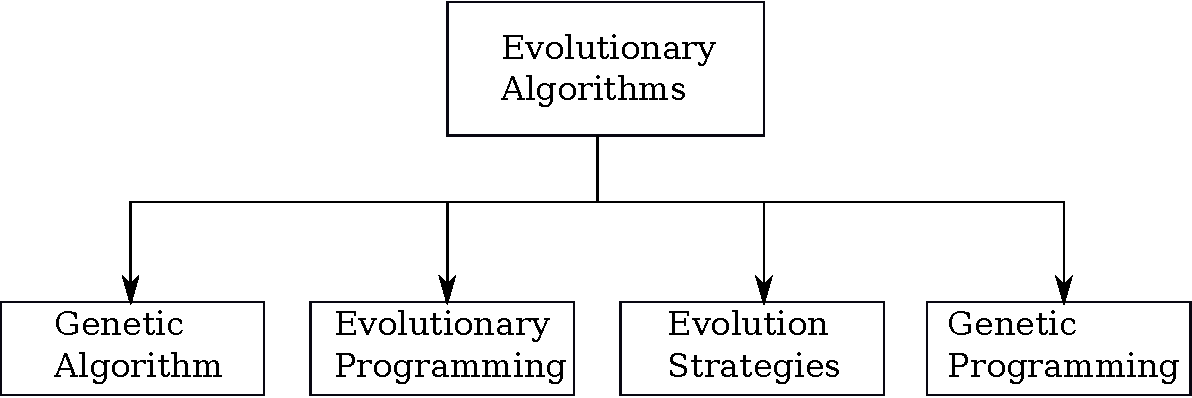
\includegraphics[width=4.2in]{evolutionary_algorithm_classification.pdf}
  \caption{Classification of evolutionary algorithms}
  \label{fig:evolutionary_algorithm_classification}
\end{figure}

The implementation of evolutionary algorithms follow a general flow during the operation process. They can be divided into $5$ steps: initialization, evaluation, mutation, selection and termination. At the beginning, a random population of individuals is initialized. These could be several random strings (chromosomes or individuals), each of which contains several genes (e.g. floating point number). These strings are encoded of the solutions we want to get. Different chromosomes are then evaluated using certain fitness function. Selection happens after the evaluation of each individual, and the ones with higher fitness normally have a higher chance of being selected to be passed to the next generation or have offsprings. The offsprings have the chance of mutation to generate new genes.  Fig.~\ref{fig:evolutionary_algorithms_flow} show a diagram of how the evolutionary algorithms proceed. 

\begin{figure}[htbp]
  \centering
  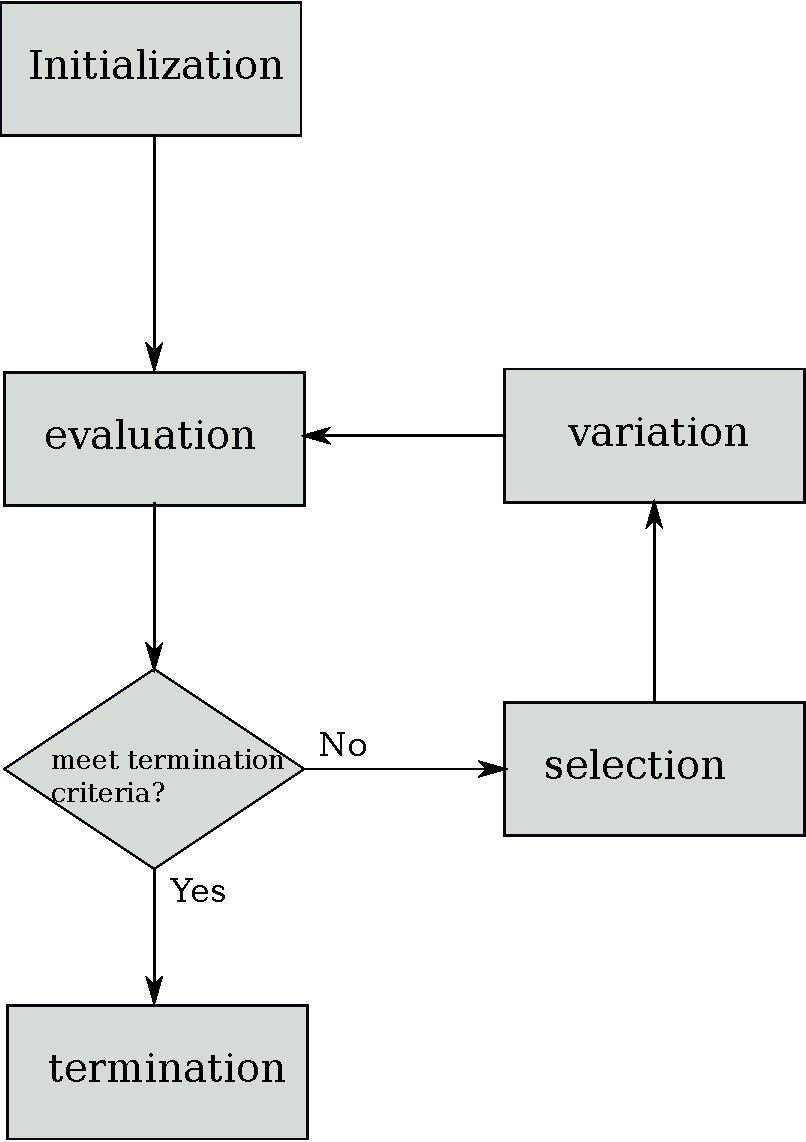
\includegraphics[width=2.0in]{evolutionary_algorithms_flow.pdf}
  \caption{This diagram shows the flow of evolutionary algorithms.}
  \label{fig:evolutionary_algorithms_flow}
\end{figure}
%For example, genetic algorithms have been applied to automatic design of mechatronic systems, complicated trading system, etc. 

\subsubsection{Coevolutionary Algorithms}

\textit{1) Principles of Coevolutionary Algorithms:} In genetic algorithm, the fitness of individuals is only decided by their own chromosomes. That means in different generations, the fitness of individuals who own the identical chromosome is constant. However, this is not true in natural coevolution. The creatures in nature are not independent, and they have different kinds of relationship as shown in Table~\ref{tab:relationship_species_coevolution}. The evolution of individuals among different species as well as evolution within the same species are coupled. Based on the idea of ecological coevolution, the coevolutionary algorithms are widely used in various research areas \cite{Rosin_1997}. Figure \ref{Fig: diagram_coevolution} shows the schematic diagram of coevolutionary algorithms between two different populations. In principle, coevolutionary algorithms can be considered of comprising several sub-algorithms, each of which could be an evolutionary algorithm. These sub-algorithms interact with each other in the fitness calculation process. In other words, the fitness of individuals in one population not only depends on its own chromosome, but also on the performance of other individuals from another population during the coevolutionary process. 

\begin{figure}[htbp]
  \centering
  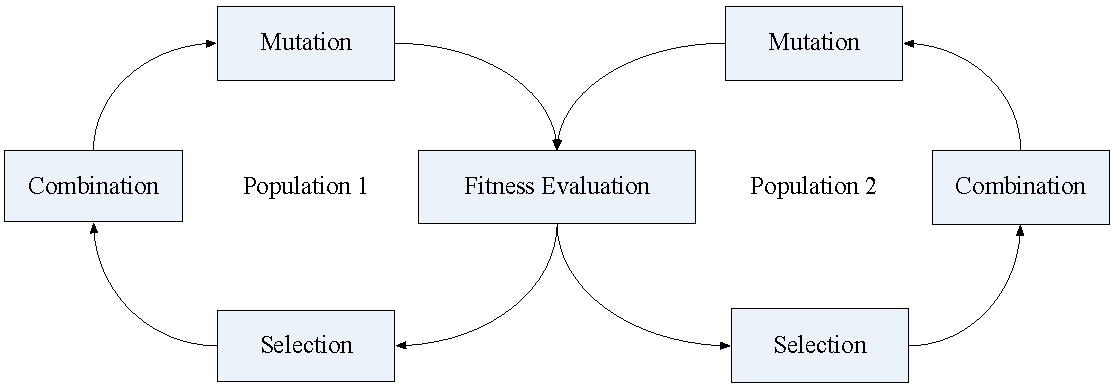
\includegraphics[width=4.2in]{diagram_co_evolution.pdf}
  \caption{Schematic diagram of coevolutionary algorithms between two different populations.}
  \label{Fig: diagram_coevolution}
\end{figure}

The essential difference between evolutionary algorithms and coevolutionary algorithms is the way of fitness evaluation. Standard genetic algorithms evaluate individuals by their chromosomes, which are independent of those in other individuals in the evolutionary system. Coevolutionary algorithms evaluate individuals based on their relative performance compared with other individuals. According to the way of evaluation, the coevolutionary algorithms are generally divided into two categories---competitive coevolutionary algorithm (Comp-CEA) and cooperative coevolutionary algorithm (Coop-CEA). Comp-CEA assesses each individual by its competitive performance with respect to its opponents, while Coop-CEA assesses each individual by its cooperative performance with respect to its co-operators. As discussed by Dawkins and Krebs \cite{Dawkins_1979}, competitive coevolution can produce a phenomena of ``arm races'' by increasing the complex of each population in the coevolution. The evolution of one species may drive another species to evolve new strategies, which makes both of the species evolve a higher level of complex behavior. Generally, Coop-CEA is applied to the situation in which the problem can be divided into several sub-problems. In Coop-CEA, thare are several cooperative species evolving simultaneously, and each sub-species represent a part of the whole solution, which is the combination of the eventual solution in each sub-species according to a certain sequence. As the~\textit{Turing learning} method presented in this thesis is based on a Comp-CEA, in the following, we introduce the fitness calculation and some pathologies of Comp-CEAs.

\textit{2) Fitness Calculation:} In coevolutionary algorithms, the fitness of individuals is called competitive or subjective fitness \cite{John_2004}. An individual's competitive fitness is based on the performance of its temporary opponents. The fitness of individuals with the same chromosome may vary because of different temporary opponents. On the other hand, the fitness in standard genetic algorithm which depends only on chromosome is called absolute or objective fitness.

In particular, there are two populations in the coevolutionary process. One is called ``learner'', and the other is called ``evaluator''. Consider L represents a set of learners, and E represents a set of evaluators. Take a learner for example. 
Its simple competitive fitness is the number of evaluators (in the current population) that this learner defeated~\cite{Angeline_1993}. It is described in equation~\eqref{equ:simple_fitness_calculation} as follows:

\begin{equation}\label{equ:simple_fitness_calculation}
\forall i \in L \Rightarrow C{F_i} = \sum\limits_{j \in E,{\kern 1pt} i{\kern 1pt} defeats{\kern 1pt} j} 1
\end{equation}

$C{F_i}$ is the fitness of learner \textit{i}. 

Another fitness calculation approach is called competitive fitness sharing \cite{Rosin_1997} as described in the following:

\begin{equation}
\forall j \in E \Rightarrow {N_j} = \sum\limits_{k \in L,{\kern 1pt} k{\kern 1pt} defeat{\kern 1pt} j} 1
\end{equation}

\begin{equation}\label{equ:competitive_fitness_sharing}
\forall i \in L \Rightarrow C{F_i} = \sum\limits_{j \in E,{\kern 1pt} i{\kern 1pt} defeat{\kern 1pt} j} {\frac{1}{{{N_j}}}}
\end{equation}

${N_j}$ represents the number of learners that could defeat evaluator \textit{j}.  

In competitive fitness sharing~\cite{Rosin_1997}, the learner that could defeat the more competitive evaluator get higher reward. For example, if a learner, $i$, in a population is the only individual to defeat an evaluator, $j$, this learner's accumulative fitness is added by $1$, as $N_j$ is equal to $1$ in Equation~\eqref{equ:competitive_fitness_sharing}.
The intention of using competitive fitness sharing is to preserve/award the learner that possesses important genetic materials which are worth passing to the next generation. 

There are many ways to choose the evaluators. Random Paring \cite{Panait_2002} means finding a random temporary opponent for each leaner. In single elimination tournament \cite{Tan_2007}, all the individuals randomly match, and the losers are taken out and winners are selected into next round of random match. Round Robin \cite{Panait_2002} means all the evaluators are the temporary opponents of each leaner. There are also other ways such as K-random opponent \cite{Tan_2007} and fitness sampling \cite{Rosin_1997}. In fitness sampling, the selected temporary opponents should have relatively higher fitness value in the last generation. The evaluation time for random paring is the shortest, but the performance is the worst; the calculation time for round robin is the longest, but the performance is the best. In our thesis, we use the simple competitive fitness calculation and Round Robin for the two populations. 

Comp-CEA can be applied in single species or multi-species. The single-species Comp-CEA is realized by competition between individuals within the same species. Any individual can be a leaner or evaluator in the coevolution process. The general Comp-CEA involves two or more species, and it simulates the predator and prey relationship in the ecological coevolution. Different species rotate as learner and evaluator during the coevolution process.

\textit{Advantages:} 

\begin{itemize}
\item \textit{Open-Ended Evolution} The competition in Comp-CEA can create an open-ended evolution for each population due to the complex interaction between the competing populations during the coevolutionary process. Such open-ended evolution could encourage the appearance of new building blocks, thus maintaining the diversity of populations. In Darwin's natural selection, this phenomenon is referred to as ``arm race''~\cite{Dawkins_1979}, which leads each species to continuously improve.  %It helps to prevent the premature convergence in the classic genetic algorithm. 

\item \textit{No Absolute Fitness} Another advantage of coevolution is when the absolute fitness of chromosome can not be effectively defined in some cases. For example, when evolving a chess playing program, it would be challenging to define a fitness to determine which program is better. A realistic way of evaluation is making the chess program play with each other and calculate the subjective fitness~\cite{Angeline_1993, David2014}. 
\end{itemize}

\textit{Pathologies:} 

\begin{itemize}
\item \textit{Red Queen Effect} During the coevolutionary process, two populations keep competing with each other. For a particular population, when~\textit{Red Queen Effect} happens, the variation tendency of subjective fitness and objective (absolute) fitness is opposite. For example, the increase of its subjective fitness may correspond to the decrease of its objective fitness. In other words, the objective fitness does increase, but the landscape of subjective fitness does not reflect such situation. 

\item \textit{Cycling} In the Comp-CEAs, the aim of each individual in one population is to defeat its temporary opponents in another population. The optimal solution which is obtained in the previous generations would probably be lost. Then after some generations, the optimal solution may be found but lost again in a few generations. The coevolution is trapped into this endless cycling, failing to find the optimal solution \cite{John_2004}. The general way of overcoming the problem of ``cycling'' is ``hall of fame''\cite{Rosin_1997}. ``hall of fame'' contains the excellent individuals of the previous generations, and chooses some of the excellent individuals as evaluators in the next generation.

\item \textit{Disagreement} During the coevolutionary process, when one species is entirely better than the other, disengagement will occur. In this case, the selection criteria won't make any sense and selection gradient will disappear, since the subjective fitness of each population is constant. The diversity of populations will converge into zero, and it is impossible to form ``arm race''~\cite{Dawkins_1979}. The common solution for solving the disengagement problem is ``resource sharing'' and ``reducing virulence''\cite{John_2004}. ``Resource sharing'' keeps the diversity of populations, and ``reducing virulence'' selects the evaluators to keep the gradient of learners' fitness.

\end{itemize}

\subsection{Applications of Evolutionary Computation}\label{sec:application_evolutionary_computation}

Evolutionary algorithms are widely used for solving various engineering tasks ranging from optimization, control, pattern recognition, robotics and system identification/modelling. In the following sections, we will focus on three main fields in which evolutionary computation technique plays a role. 
%Such algorithm has been successfully applied in intelligent games, for example, Tic-Tac-Toe \cite{Angeline_1993} and function optimization \cite{Tan_2007}. The multi-species Comp-CEA has been successfully applied in intelligent games such as Tic-Tac-Toe \cite{Rosin_1997}, function optimization, multi-objective optimization \cite{Tan_2007}, pattern recognition, the design of nonlinear controllers and artificial neural networks \cite{Floreano_1997}.

\subsubsection{Black Box Optimization}

\begin{figure}[!t]
  \centering
  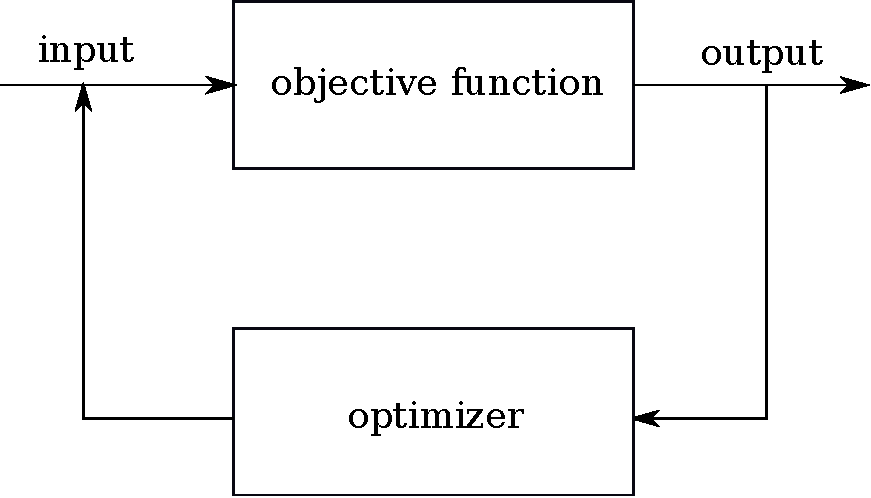
\includegraphics[width=3.2in]{black_box_optimization.pdf}
  \caption{This diagram shows the process of black box optimization. The task is to find a candidate solution (input) that can optimize (e.g. maximize or minimize) the objective function.}
  \label{fig:black_box_optimization}
\end{figure}

One of the promising application of evolutionary computation is black box optimization. Black box optimization refers to such problems that the optimization algorithm aims to optimize an objective function without assuming the hidden structure of that function (e.g., linear or differentiable). In particular, the aim is to found a set of inputs that can maximize or minimize the output of the objective function. For example, in a traveling salesman problem (a combinatorial optimization), in which the task is to find the best combination of route of cities (input) that can minimize the length of tour of visit all cities (objective). Fig.~\ref{fig:black_box_optimization} shows a diagram of the black box optimization.

Due to the complexity of the real problem in nature, the stochastic search algorithm such as evolutionary algorithms provide us an efficient and relatively `perfect' solutions. Although evolutionary algorithms could not guarantee the best solution would be found every time, they are still superior to many traditional search algorithms such as the greedy local search algorithm~\cite{Gutin200281}. There are many real-world examples that using evolutionary computation techniques to solve the optimization problem. In the area of nanophotonic light trapping, an urgent need is the development of low cost thin film solar photovoltaic technologies. A traditional way is fixing the structure according to the physical intuition and trying to find the optimal parameters. In~\cite{Wang2013}, a highly efficient light-trapping structure was designed using a genetic algorithm. It was shown that this new structure can increase the trapping efficiency three times comparing with the classic limit. The high efficiency achieved by the new design is far beyond the reach of traditional design. Another successful example is using evolutionary algorithms to design antennas for NASA's Space Technology spacecraft~\cite{Hornby2011}, and one of the antennas was used in the mission. The antennas is a critical device for the spacecraft to communicate with the ground, as faulty communication may cause a lot of data lost or the crash of the spacecraft. The antennas designed using evolutionary algorithms are significantly better than those designed by human experts. Another advantage of using evolutionary algorithms for designing is once the fitness function was changed, it can quickly come up with another design can fit the purpose. 

In the following, we list several cases (but not all) that evolutionary computation could be applied to solve the `tough' optimization problem. 

\begin{itemize}

\item \textit{High-dimension} As the dimension, $n$, of the objective function increases, the search space increases exponentially. This is called ``curve of dimension'' by Bellman~\cite{Bellman1957}. For example, if we have to optimize a function that has $30$ dimensions, and each dimension only has $20$ parameters to be selected. For a grid search in which all the possible solution is evaluated, it will take $20^{30}$ evaluations. Suppose that each evaluation takes $1\mu s$, it would more than the $3\cdot 10^{31}$ years. However, if using evolutionary computation, it probably takes hours to find the optimal solution. 

\item \textit{Multi-Model} Multi-model means a system (function) has more than one optimums (e.g., Rastrigin Function). The one/s with the best fitness value is/are considered as global optimum/s, and the other are considered as local optimums. 
These local optimums around the global optimum/s are very misleading for the gradient-based search algorithms (e.g., \textit{hill climbing} algorithm), as the solutions may easily get trapped at the local optimums. Evolutionary algorithms are shown to be very efficient to find the global optimum/s. %For example, in the optimization of a multi-layer forward neural network, there may be multiple representations that could produce the same output because of the symmetrical structure of the hidden neurons.

\item \textit{Non-separable and non-differential} A function, $g(x_1, x_2, \cdots, x_n)$ is non-separable, if it can not be expressed as: $g(x_1, x_2, \cdots, x_n) = g(x_1)g(x_2) \cdots g(x_n)$. For the separable function, it would be much easier to optimize, as we can treat each variable separately. However, for non-separable system, the variables are normally coupled. Also, the function may not be differential, which makes many mathematical optimization algorithms (e.g., quasi-Newton BFGS algorithm~\cite{Dennis1977} or conjugate gradient algorithm~\cite{Shewchuk1994}). The state-of-the-art of the evolutionary algorithm for black box optimization in contentious domain is Covariance Matrix Adaptation Evolution Strategy (CMAES)\cite{Hansen2003}.

\item \textit{Multi-objective} When encountering real-world problem, we usually need to deal with multiple objectives, which need to be optimized simultaneously. For example, when designing a car, the engineers need to consider the shape, performance of the engines, and more importantly cost. As some of the objectives (such as performance and cost) are conflicting, the designer needs to find a Pareto optimal solution, in which none of the value of the objective functions can not be increased without considering decreasing the value of other objectives. Evolutionary multi-objective optimization is an efficient technique for generating such Pareto optimal solutions for multi-objective optimization problems. For a review, see~\cite{Fonseca1995}. 

\end{itemize}

\subsubsection{Evolutionary Robotics}\label{sec:evolutionary_robotics}

Another application of evolutionary computation is evolutionary robotics, in which the controller and/or morphology of the robots are automatically generated. The user considers the robot as a whole and only needs to specify the criterion which is represented by a fitness function. The fitness function could be single-objective or multi-objective. The aim is to optimize (minimize or maximize) the fitness using evolutionary algorithms. The normal procedure of evolutionary robotics is as follows. First, an initial population of random controllers are generated. Each controller are represented by a chromosome. If the controller is a neural network, the chromosome is a vector of real numbers. Each controller was imported into the robot(s), and the robot's performance when performing various tasks is measured and evaluated using the pre-defined fitness function. After some genetic operators (e.g. crossover, mutation), the `fitter' robot controller has a higher chance of being selected and generating offspring in the next generation. This process iterates until a good solution is found. 

In contract to evolutionary robotics, another method of designing robot controller and/or morphology is behavior-based approach, where the designer divides the whole system into several simple parts intuitively. These separate parts are then integrated all in once through a coordination mechanism---competitive or cooperative coordination~\cite{Brooks1986}. In competitive coordination, only one part has an effect on the output of the robot, while in cooperative coordination, several parts contribute to the output of the robot with different weights. The behavior-based method was shown to be very robust in many tasks such as gait control in locomotion and object transport. The challenge of designing robot controller and/or morphology using behavior-based method is it requires a lot of experience from the designer. Moreover, when the system is highly coupled, separating the whole design into different parts may not be a good strategy. However, evolutionary robotics provides the designer an alternative way of controlling the robot as a whole, rather than focuses on the details of each separate component. The synthesized control system is a result of self-organized process. %A schematic diagram showing the design process of evolutionary method and behavior-based method is shown in Fig.~\ref{}.

There are many control structure that can be adapted in evolutionary robotics. One popular structure is artificial neural network due to its simple representation and strong power of control. The tree-based structure like LISP is also very robust, and it is widely used in evolutionary programming~\cite{Koza:1992}. The \textit{building blocks} method was proposed by Brooks~\cite{Brooks92artificiallife}. However, these blocks are described using high-level languages, which are are suitable for evolution in the low level. Comparing with other control structures, artificial neural network have many advantages~\cite{Floreano_1997, Floreano2008:NN}. According to the types of behavior (e.g., simple perception or non-linear dynamic), we can choose different neural networks (forward neural networks and recurrent neural networks, etc.). Recent development reveals that we can even evolve the topology and weights of the neural networks~\cite{Kenneth2002}. 

There are two main research aims in evolutionary robotics: 1) engineering---developing the control strategy for robots; 2) biology---to understand the biological systems using simulated evolution. In engineering, a range of work has been presented, ranging from simple behaviors, such as phototaxis behavior, self-charging behavior to complex behaviors such as navigation and locomotion of robot with multiple degrees of freedom. In biology, evolutionary robotics is used as a tool to understand the general principles of evolution. It provides much more efficient and faster way to validate or even create hypothesis based on evolution in simulation or real robots, compared with the slow evolutionary process in nature. AVIDA~\cite{Bryson2013} and AEvol~\cite{Batut2013} are two computer software systems that are used for studying the evolution of bacterial. In hypothesis validation, evolutionary robotics was used as a tool to investigate some key issues in biology. For example, whether altruistic plays an important role in cooperation~\cite{montanier:inria2011,Waibel2011}, the conditions of emergence of communication during the evolution~\cite{Floreano2007514}, and how morphology and control are coupled~\cite{Auerbach:PLoS:2014}, coevolution of predator and prey~\cite{Cliff_1995, Floreano_1998}. 
%In the simulation or experiments, some interesting behaviors which are similar to those in nature can be found and analyzed. For example, in~\cite{Floreano_1998}, the predator tries to catch the prey, while the prey tries to escape from the predator. Both species evolve more and more complicated behaviors in order to compete with each other.

Using evolutionary algorithms to generate a desirable behavior/result requires a relatively large population size and certain number of generations. Therefore, performing evolution on the real robot would take plenty of time. The initial experiments may also cause damage to the robot itself or the environment the robot is operating on. Therefore, a lot of experiments/evaluations are performed in simulation. As the simulator can not match the reality, the controller generated in simulation may not work well in reality, causing \textit{reality} gap. Some work are done to reduce the \textit{reality gap}. In~\cite{Koos:TEVC:2013, Koos:IJRR:2013}, the author uses the transferability approach to increase the quality of controller generated in simulation through reducing the gap between simulation and reality. In~\cite{Floreano1996}, the evolution is even performed directly on the real robot to evolve the controller to perform navigation task. However, the battery is still a problem as it takes two weeks to evaluate $100$ generations. The addressed this issue through connecting a wire between the robot and the power station. 

Recently, a distributed online onboard evolutionary method (artificial embodied evolution) has received much attention~\cite{Watson2012, eiben:inria-00531455, Eiben:EI:2012}. In artificial embodied evolution, the population is distributed among different robots, and the gene exchange is done through \textit{mating}. Each robot only exchange its genes with its nearby neighbors. There is not central control over the group of robots. This approach is particularly suitable for the situation where the environment that the robots are operating on is not predictable or changing after deploying the robots. The robots need to evolve to adapt to the changing environment, while satisfying certain basic requirements inserted by the designers. A more challenging research area could be evolving both the morphology and controller of the robots in a distributed manner---\textit{evolution of things}~\cite{Eiben:Nature:2015}. This forms an open-end evolution among different artifacts, which is a process how living creatures evolve in real world. The fast development of 3D printing technique makes this method appealing~\cite{Tumbleston20032015}. 

\subsubsection{System Identification}

System identification which is about building the model of a hidden system through conducting a set of experiments is widely used in both academic and industrial areas \cite{Ljung_1999}. The experiments are conducted by a series of inputs into the system and the outputs corresponding to the inputs are collected. The process of system identification is to find a model that fits the inputs and output. It is composed of observed data, model structure, a criterion to evaluate different models according to the observed data, validation of the obtained model based on different data set, and revision of model if necessary. 

There are two system identification approaches: the offline approach and online approach. In the offline approach, the observation data is collected first, and the aim of modeling is to generate a model that fits the observed data. This method is often used when the data is easy to collect or the parameters and operating environment of the system do not change too much in a short time. However, in some cases, the parameters of the system are always changing due to different operating environment. That means the obtained model based on the previous observation data can not be applied to the new situation any more. In this case, the model should be updated using the new observed experimental data and online system identification method. The two approaches of system identification are shown in Fig.~\ref{fig:modeling_approaches}. Note that for some systems, there are only outputs.
 
\begin{figure}[!t]
  \centering
  \subfloat[]{
  	  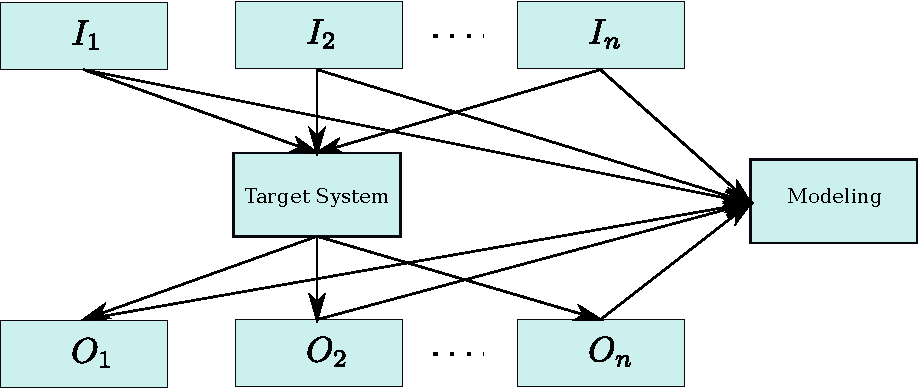
\includegraphics[width=2.5in]{system_identification_approach_offline.pdf}
  }\\
  \subfloat[]{
  	  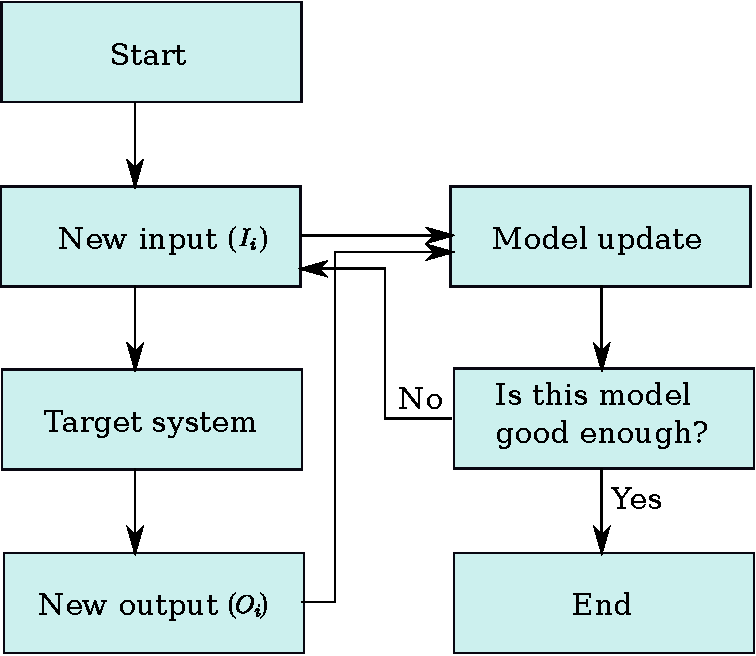
\includegraphics[width=2.5in]{system_identification_approach_online.pdf}
  }
  \caption{The diagram showing the two approaches ((a): offline; (b): online) for system identification. $(I_i, O_i)$, where $i \in [1, 2, \cdots, n]$, represents a pair of input data and output data.}
  \label{fig:modeling_approaches}
\end{figure}

System identification can be divided into two main procedures: modeling and estimation. Modeling defines the order or general structure of the hidden system \cite{Fogel_1991}. Estimation identifies the parameters associated with the given structure. There are many estimation algorithms to determine the parameters for a given structure. Typical estimation algorithms are recursive prediction error methods which are based on gradient search. Gradient search method such as greedy algorithm can easily get trapped in local optima, especially when there are numerous local optimal points near the global optima. An alternative search method is using evolutionary algorithms. As evolutionary algorithms use population-based search method, this makes it more likely to get rid of local optima. 

There are also some system identification methods that combine the modeling and estimation process, e.g., NARMAX method~\cite{Billings2013}. Neural network is a good representation of the system under investigation, as its topology and weights can be optimized simultaneously. The disadvantage of neural network is it is hard to interpret the obtained model when there are multiple layers, which makes it much hard to analyze the target system. Genetic programming provides an alternative way for finding the structure and parameters of the system. The model represented by genetic programming is described in a tree-based structure. As the structure in genetic programming is evolving, the obtained model may have different structure in different runs~\cite{Vladislavleva:2009}. Bloating is a problem in genetic programming, where the growth of the tree increases the complexity of the model structure. 

Coevolutionary algorithms provide an effective way for system identification~\cite{Bongard2005}, \cite{Bongard_remote_robot_2004,Bongard_function_recovery_2004,Koos2009,Bongard2007PNAS,Mirm2011,Ly2014}. A range of work have been performed on simulated agents. In~\cite{Bongard_remote_robot_2004}, Bongard and Lipson proposed the \emph{estimation-exploration algorithm}, a nonlinear system identification method to coevolve inputs and models in a way that minimizes the number of inputs to be tested on the system. In each generation, the input that leads to the highest disagreement between the models' predicted output in simulation was carried out on the real system. The quality of the models was evaluated through quantitatively comparing the output of the real system and the models' prediction. The method was applied to evolve morphological parameters of a simulated quadrupedal robot after it undergoes `physical' damage. In a later work~\cite{Bongard_function_recovery_2004}, they reported that ``in many cases the simulated robot would exhibit wildly different behaviors even when it very closely approximated the damaged `physical' robot. This result is not surprising due to the fact that the robot is a highly coupled, non-linear system: thus similar initial conditions [...] are expected to rapidly diverge in behavior over time''. They addressed this problem by using a more refined comparison metric reported in~\cite{Bongard_function_recovery_2004}. In~\cite{Koos2009}, an algorithm which is also based on coevolution of models and inputs was presented to model the simulated quadrotor helicopter and improve the control quality. The inputs were selected based on multiobjective performances (e.g., disagreement ability of models as in ~\cite{Bongard_remote_robot_2004} and control quality of a given task). Models were then refined through comparing their prediction to each selected test trajectory. In~\cite{Kouchmeshky_2007}, the damage detection process is conducted by coevolutionary algorithm to extract the maximum information from the system. In \cite{Mirmomeni_2011}, coevolutionary algorithm is applied to estimate chaotic time series, in which the test data that can extract information from the chaotic system co-evolves with the models. In these works, predefined metrics are critical for evaluating the performance of models. 
  
Many studies also investigated the implementation of evolution directly in physical environments, on either a single robot~\cite{ Bongard-etal2006:science, Koos2013, Cully2015} or multiple robots~\cite{Alan2014}. In~\cite{Bongard-etal2006:science}, a four-legged robot was built to study how it can infer its own morphology through a process of continuous self-modeling. The robot ran a coevolutionary algorithm on-board. One population evolved models for the robot's morphology, while the other evolved actions (inputs) to be conducted on the robot for gauging the quality of these models through comparing sensor data collected. In~\cite{Alan2014}, a distributed coevolutionary approach was presented to coevolve on-board simulators and controllers of a swarm of ten robots to perform foraging behavior. Each robot has its own simulator which models the environment. The evolution of each robot's simulator was driven by comparing the real-world foraging efficiency (a pre-defined fitness metric) of its nearby neighbors each executing the best controller generated by their own simulators. Each robot has a population of controllers, which evolved according to the robot's on-board simulator. The best controller was chosen for performing real-world foraging. This physical/embodied evolution helps reduce the \textit{reality gap} between the simulated and physical environments~\cite{Jakobi95}. In all of the above approaches, the model optimization is based on pre-defined metrics (explicit or implicit), which are task dependent.

%In \cite{Kouchmeshky_2007}, the damage detection process is conducted by coevolutionary algorithm to extract the maximum information from the system. In \cite{Mirmomeni_2011}, coevolutionary algorithm is applied to estimate chaotic time series, in which the test data that can extract information from the chaotic system co-evolves with the models. The approach described in~\cite{SchmidtLipson2009:science}, where the authors infer physical laws from observing mechanical systems, would also be applicable to learn about the behavior of an animal. Different from this approach our system learns about the behavior not through passive observation, but rather through an interactive process.

\section{Combining AI/Robotics and Animal Behavior}\label{sec:combine_AI_robotics_animal_behavior}

The variety of animal behaviors in nature is immense, ranging from simple perception to complicated behaviors such as navigation and communication. The scientific study of animal behavior is pursued not only because it is a subject of interest in itself, but also because the knowledge gained from it has several practical applications. In AI/Robotics, there is a large interest of studying animal behavior, as the model/knowledge learned can be used to build a more intelligent machine. At the same time, building machine that mimics the animal helps us better understand its behavior. In this section, we review how AI/robotics and animal behavior study benefit each other. In Section~\ref{sec:animal_behavior_in_nature}, we introduce some interesting animal behaviors observed in nature. In Section~\ref{sec:swarm_optimization_swarm_robotics}, we detail how the animal behavior observed in nature can be used as inspiration for solving engineering tasks, especially in the area of AI/robotics. In Section~\ref{sec:contribution_of_AI/robotics_to_ethology}, we show how AI/Robotics can contribute to the study of animal behavior, which is the theme of this thesis.

\subsection{Animal Behavior in Nature}\label{sec:animal_behavior_in_nature}

\subsubsection{Single Behaviors}

Comparing with the behaviors exhibited by complex animals such as mammals, insect behavior arises a large interest both by biologists and roboticists. One reason is due to the simple neural system of the insects, which provides a good inspiration for engineering purpose. This simplicity also makes it easy to replicate the intelligence exhibited by the insects. 

A basic insect behavior is taxis, which is its intrinsic behavioral response to a specific stimulus. Taxis is divided into different type according to the stimulus which elicits the response. These behaviors include phototaxis (light), chemotaxis (chemicals), thermotaxis (temperature), etc. For example, a lobster follows the salt-water plume---a kind of chemical signal to find its source. Another interesting taxis behavior of crickets is that the female crickets perform complex auditory orientation behavior towards the male crickets. Researchers have found this complex sound localization behavior emerge from simple reactive steering responses to specific sound pulses generated by male crickets~\cite{Hedwig2004}. Apart from taxis behaviors, some insects use the stimuli as cues for navigation or migration. For instance, the bee uses its vision system to navigate in the air and avoid obstacles. Another interesting behavior found in insects is the ball movement of dung beetles~\cite{Emily_2012}. Once the dung beetles form the pieces of dung into a ball, they always roll the dung-ball in a straight line using various stimuli (e.g., the moon, sun and polarised light \cite{Byrne_2003, Matthews_1962}) as visual cues to transport the food source. This behavior ensures that they keep away from the competitors as far as possible. 
 
The stimulus-response behaviors in insects mentioned above are investigated by biologists for centuries. When investigating such behaviors, biologists need to learn how to interact with the animal in a meaningful way to extract all the behavioral repterio of the insect under investigation. However, whether this interacting ability could be exhibited by an intelligent machine is still an uncertain problem, which is addressed in this thesis. 

\subsubsection{Swarm Behaviors}

Apart from single-animal behavior, swarm behaviors, which are emergent (collective) behaviors that arise from the interactions of a number of animals (especially social insects) in a group, have also been widely observed in nature. The individual behaviors in a swarm tend to be relatively simple~\cite{Camazine2001}. The global behavior that is exhibited in a swarm is a result of self-organized process. Researchers found that individuals do not need the representation or complex knowledge to build a map of what the global behavior should be~\cite{Garnier:SI:2007}. There are no leaders in the colony. From the point of control, swarm behavior is a distributed control system which does not rely on central coordination.

Many swarm behaviors are observed in nature. For example, the flocking behavior of birds are of particular interest to humans. This is not only because of their beautiful shape formed in a group, but also how the birds coordinate with each other to maintain that shape. A simple mathematical model was proposed by~\cite{Craig:CG:1987} to describe the individual behavior of each bird in a flocking. The three rules are: attraction, repulsion and alignment. In the attraction rule, the birds will be attracted by their neighbors, and this would result in each bird moving towards to the `center' of their neighbors. Repulsion means the bird needs to avoid colliding with each other. Alignment assumes that each bird moves in the same direction with its neighbors. Although there is no prove that flocking birds follow exactly these three rules, it is attractive that the boids (in simulation) following such simple rules can mimic the real flocking behavior very closely. There are many some other swarm behaviors which are also studied extensively such as the aggregation of cockroaches~\cite{Jeanson:AB:2005}, foraging in ants~\cite{Carroll1973}, flashing synchronization in fireflies~\cite{James:ARE:1971}, mound building in termites~\cite{Bruinsma:PHD:1979}. 

\subsection{Swarm Optimization and Swarm Robotics}\label{sec:swarm_optimization_swarm_robotics}

In the previous sections, we introduce some interesting animal behaviors observed in nature. Many algorithms are inspired from observation of animal behaviors. In this section, we will review two main optimization algorithms inspired from swarm behaviors---ant colony optimization algorithm~\cite{Dorigo_1997} and particle swarm optimization algorithm~\cite{Kennedy:ICNN:1995}. Swarm robotics is another application area which uses the swarm behaviors of social animals as an inspiration to solve complex tasks using multiple robots. 

\subsubsection{Swarm Optimization}

\textbf{Ant Colony Optimization}

Ant Colony Optimization (ACO) is an optimization technique that gets inspiration from foraging behavior of ants. When ants go out to search for food, they will leave pheromone in the path. Ants will be attracted by the pheromone, the strength of which represents the quality of the food source. Researchers have found that this indirection communication, which is know as \textit{stigmergy}~\cite{Holland:AL:1999}, leads them to found the shortest path along their nest and location of food source. The initial application of ACO is to find the optimal path in the combinational (discrete) problem. Note that nowadays the application of ACO algorithms ranges from network optimization (e.g., routing and load balance~\cite{DiCaro:JAIR:1998}) to continuous optimization~\cite{Dorigo:LNCS:2004}.   

The principle of ACO algorithms can be divided into the following two steps:

\begin{itemize}
\item Use the pheromone model to generate condidate solutions. From the aspect of mathematics, the pheromone model is a parameterized probability distribution in the search space.

\item The candidate solutions are used as a bias for the future sampling to get better solutions.
\end{itemize}

\textbf{Particle Swarm Optimization}

Particle Swarm Optimization (PSO) is another an optimization algorithm which gets inspiration from flocking of birds or schooling of fish. It was first proposed by Kennedy and Eberhart~\cite{Kennedy:ICNN:1995}. The initial application is to optimize the weights of neural networks---a continuous optimization problem. It is also widely used in discrete optimization. 

The basic component in PSO is called \textit{particle}. A PSO algorithm consists of a finite set of particles. The movement of each particle is updated using \textit{velocity}. The velocity of each particle in each time step is updated based on its current velocity, the deviation between the best position (it has found so far) and its current position, and deviation between the best position by its neighbors and its current position. This will result in the particles moving towards the high-quality solutions after certain iterations. The update of each particle can be written using two equations as follows:
\begin{equation}\label{eq:particle_velocity_update}
\overrightarrow{v}_{i+1} =  \overrightarrow{v_{i}} + c_1\overrightarrow{R_{1}}\otimes(\overrightarrow{p_{i}} - \overrightarrow{x_{i}}) + c_2\overrightarrow{R_{2}}\otimes(\overrightarrow{p_{g}} - \overrightarrow{x_{i}}) 
\end{equation} 

\begin{equation}\label{eq:particle_position_update}
\overrightarrow{x}_{i+1} =  \overrightarrow{x_{i}} + \overrightarrow{v_{i}}
\end{equation} 

where $\overrightarrow{R_{1}}$ and $\overrightarrow{R_{2}}$ are independent random number generators that return a vector of random values in range $[0, 1]$. $c_1$ and $c_2$ are referred to as acceleration coefficients. The first item in Eq.~\eqref{eq:particle_velocity_update} keeps the particle moving in the previous direction; the second item makes the particle move towards the best position of its own; the third position forces the particle move towards to the best position that its neighbors have found. Eq.~\eqref{eq:particle_position_update} updates the particle's position.  

\subsubsection{Swarm Robotics}

In the previous sections, we talk about how swarm behaviors can be used as inspiration for algorithms design. In this section, we introduce how to use swarm intelligence techniques to multiple robots research, which is referred to as swarm robotics. Many social insects' (e.g, ants, termites, wraps and bees) behavior can be used as inspirations in swarm robotics. 

Swarm robotics investigates how multiple robots each with limited ability communicate, coordinate and self-organize to accomplish complex tasks. To finish the same task, using a single expensive robot with complex control structure may be feasible but it may have low efficiency and prone to failure. The advantages of swarm robotics are as follows: 

\begin{itemize}

\item \textit{Robustness} A swarm system consisting of multiple robots is robust in term of failure of certain robots disturbance of the environment. This robustness can be explained in the following reasons: 1) if some robots failed, the other robots would replace the functions of the failed robots; 2) the control is distributed; 3) as the individual is simple, it is less likely to be damaged; 4) the perception from multiple robots would increase the system's robustness. Note that in some swarm systems, there may be exceptions. That is, some individual failure would influence the whole self-organized process~\cite{Bjerknes2013}.

\item \textit{Scalability} In swarm robotics, the number of robots do not have significant difference on the global performance/behavior in the system. That is, increasing/decreasing certain number of robots, the system is still under control and the coordination is maintained. When investigating a swarm robotic system, scalability study is usually considered~\cite{Jianing:TRO:2015, Melvin_DARS2014}.

\item \textit{Flexibility} The swarm could easily adapt to the changing tasks and generate relevant solutions~\cite{Sahin:LNCS:2005}. The role of each robot in the swarm could be changed depending the need for the task. 
\end{itemize}

In order to cooperate, the robots need to interact with each other and environment. There are three kinds of interaction in swarm robotic systems. 

\begin{itemize}

\item \textit{interaction via environment} In this interaction method, the robots communicate with each through changing the environment. There is no explicit communication between each robot (i.e., they do not exchange message). In nature, this method is observed in social ants. The pheromone they leave when foraging is an environmental stimulus for locating the food source.  

\item \textit{interaction via perception} In this method, the robots can perceive each other in a limited range. This perception is local and there is no explicit communication between each robot. This requires the robots can distinguish between robots and objects in the environment. In nature, when the ants need to collectively pull the food to the nest, they need to perceive each other (to avoid collision) and the food (object).

\item \textit{interaction via explicit communication} In this method, a network is required to communicate with a swarm of robots in real time. This could be done by broadcast (e.g., WiFi~\cite{Gerkey:TRA:2002}) or a distributed sensing network~\cite{Winfield:LNCS:2000}. How to build a reliable network when the number of robots is significantly large is still a hot topic widely discussed. When the number of robots increases, the load of communication increases exponentially. A possible solution is combining the advantage of network communication and local communication using the robots' perception.

\end{itemize}

A range of tasks have been demonstrated in swarm robotics. The tasks range from aggregation~\cite{Trianni:LNCS:2003, Gauci2014_ijrr, Garnier:AL:2008, Jeanson:AB:2005}, dispersion~\cite{howard2002mobile, mclurkin2004distributed}, pattern formation~\cite{Fujibayashi:DARS:2002, Chen:AAMAS:2012}, collective movement~\cite{Turgut:SI:2008} to cooperative transport~\cite{Kube:AB:1993, Kube:RAS:2000,Gross:IJBC:2009, Jianing:TRO:2015}, etc. Aggregation can be considered as the fundamental behavior of other more complex tasks. In~\cite{Jeanson:AB:2005}, a group of robots mimic the cockroaches' aggregation behaviors, in which the robots gather into or leave the nest with a probability proportional to the size of the nest. The advantage of using stochastic algorithm is that they do not need to form a connected network in the initial configuration. In~\cite{Gauci2014_ijrr}, the robots each with a binary sensor were reported to aggregate into a single cluster, validated using $40$ e-puck robots. The robots do not need to perform algorithmic computation. This work was scaled well using $1000$ robots in simulation. In~\cite{Werfel:Sci:2014}, Werfel et al. designed a group of termite-inspired robots that work collectively to build several structures. The robots communicate with each other using \textit{stigmergy}. In~\cite{Turgut:SI:2008}, a group of nine Kobot robots were reported to mimic the flocking behavior of birds. These robots followed some simple rules similar to those proposed by Reynolds~\cite{Craig:CG:1987}. In cooperative transport, Chen et al.~\cite{Jianing:TRO:2015} proposed a strategy in which the robots only push the object when the robots' vision of the goal is occluded by the object. This strategy was proved to push any convex object in a plenary environment. 

\subsection{Contribution of AI/Robotics to Ethology}\label{sec:contribution_of_AI/robotics_to_ethology}

In the previous sections, we reviewed how animal behavior study can be used as inspiration for designing algorithms and robotic systems. However, robotics can also benefit animal behavior study. In this section, we review two approaches in AI/robotics to contribute to the study of animal behavior: \textit{learning from synthesis} and \textit{robot-animal interaction}.

\subsubsection{Learning from Synthesis}

Ethologists have studied animal behavior over a century. However, even some basic behaviors such as taxis (which is widely observed in animals such as insect larvae and worms~\citep{Fraenkel:DP:1961, Stephen:Op:1990}) is still not completely understood \cite{Rano_2009}. There are some basic steps that ethologists follow in the study of animal behavior~\cite{camazine2003self}. The first step is observation, and after that they formulate some scientific questions on the observed behavior, and generate hypothesis to answer these questions. In order to verify the hypothesis, they actively conduct related experiments in the real animals and collect certain amount of data. After analyzing the data, the conclusion will be made to support or reject their hypothesis.

Robotics or artificial life can be used as an alternative methodology to investigate and understand animal behavior. Robots can be used as physical models of animal behaviors for testing hypotheses~\citep{Barbara_2000, Meyer2008}. For example, taxis behavior has often been implemented on mobile robotic systems. Webb~\citep{Barbara_1995} used a robot to model the phonotaxis behavior of crickets~\citep{Popov:JCP:1997}. The robot can locate the position of a sound source and move towards it under different conditions. There was a good agreement between data collected from experiments on the robot and the animal. Another taxis behavior---chemotaxis in which animals follow a specific chemical trial has been used as a model for robots to find odour source based on artificial neural networks \cite{Farah_2002} and even Braitenberg vehicles \cite{Lilienthal_2003}. Robots can be used as a validation for the models obtained from biologists and allow them to better understand the animal behavior from a synthetic point of view.  Besides, roboticists can generate new hypotheses and test them using (simulated or real) robots.
 
In social behaviors study, Balch et al.~\citep{Balch_2006} built executable models of the behaviors and ants and monkeys, which can be directly executed by multi-robot systems. The aim is to show how research into multi-robot systems can contribute to the study of collective animal behaviors. Besides robotics, there are some researchers arguing that artificial intelligence can also make significant contributions to biological study. In \cite{Chappell_2010}, Chappell et al. argue that there are many ways in which biologists interested in natural intelligence can learn from AI, and they outline the many specific kinds of contributions that AI can make to biological study. They also give some suggestions on how AI researchers collaborate with biologists to combine the advantage of each other and solve some cutting-edge problems in animal behavior.

As opposed to the works mentioned above, the method proposed in this thesis aims to synthesize models of animal (agent) behaviors automatically, rather than manually. This could help to spare scientists from having to perform numerous laborious experiments, allowing them instead to focus on using the generated models to produce new hypotheses and conduct further experiments. 

\subsubsection{Robot--Animal Interaction}\label{sec:robot_animal_interaction}

Besides pure robot-based or AI research, researchers also use robots to interact with real animals. They build and programme robots (i.e., replicas) that can be inserted into the group of social animals~\cite{Faria2010, Halloy2013, J.Halloy2007, Thomas2013, Vaughan2000}. Robots can be created and systematically controlled in such a way that they are accepted as con- or hetero-specifics by the animals in the group~\cite{Krause2011}. In this case, one ``animal'' in a group is completely controlled and they can observe the behaviors of the mixed society \cite{J.Halloy_2007}. The behavior of the inserted robot can be controlled and the model can also be embedded into the robot for verification \cite{Krause_2011}. The behavior of robots can be programmed in such a way that its behavior is not influenced by the other real animals in the group, and they can be used as demonstrators or leaders in the experiments. Further more, it is easier to verify a hypothesis through controlled interaction in social behaviors. 

For example,  in~\cite{Faria2010}, a replica fish which resembled the appearance (i.e., visual morphology) of sticklebacks was created to investigate two types of interaction: recruitment and leadership. In~\cite{J.Halloy2007}, autonomous robots which executed the derived model were mixed into a group of cockroaches to modulate their decision-making of selecting shelter in the aggregation behavior. The robots behaved in a similar way to the cockroaches. Although the robots' appearance was different to that of the cockroaches, the robots released a specific odor that the cockroaches could detect and regard the robots as conspecifics. In \cite{Vaughan_1998, Vaughan2000}, Vaughan et al. have built a mobile robot that can interact with the ducks in a circular arena and drive them to the safe place. Halloy et al. In \cite{Gribovskiy_2010}, Gribovskiy et al. designed a robot which is capable of interacting with chicks to study how the behavior of chicks can be influenced by the others in a group. Although robots which are well designed can be mixed in social animals, building such kind of robot is a time-consuming process. It is also expensive to some extent and requires the collaboration of researchers from different disciplines. In~\citep{Kopman2013}, a robot-fish that can interact intelligently with live zebrafish to study their preference and locomotion behavior was designed . 

In these works, the models were manually derived and the robots were only used for model validation. We believe that this robot-animal interaction framework could be enhanced through \textit{Turing learning}, which autonomously infers the collective behavior. 

\clearpage 

%The research of animal behavior has lasted for centuries. There are some basic steps that ethologists follow in the study of animal behavior. The first step is observation, and after that they formulate some scientific questions on the observed behavior, and generate hypothesis to answer these questions. In order to verify the hypothesis, they actively conduct related experiments in the real animals and collect certain amount of data. After analyzing the data, the conclusion will be made to support or reject their hypothesis. Take the behavior of dung beetle for instance. An interesting feature observed by ethologists in the behavior of dung beetles is that they always roll the dung-ball in a straight line. This strategy guarantees that the beetles can roll the dung as far as possible in the shortest time, ensuring that they can escape from the competition or danger that may occur near the cite of dung \cite{Emily_2012}. Previous works show that the most significant cues which dung beetles use for navigation -- straight line movement are the moon, sun and polarised light \cite{Byrne_2003, Matthews_1962}. In \cite{Dacke_2004}, Dacke, et al. study how dung beetle \textit{Scarabaeus zambesianus} orientates due to the artificial polarization pattern instead of observing the behavior in the natural polarized light, since it is quite easy to control the angle when using artificial light source. To do the experiment, they put the dung beetle in a squared arena. When the beetle enters the central point, they switch the angle of the artificial light source from 0 degree to 90 degree to interact with the dung beetle. Then they observe the path taken by the rolling dung to see whether the angle of light source has influence on the beetle's orientation behavior. The light switching process is very time-consuming, and the researchers have to change the angle of light source for many times (90 times, if the angle increases one degree each time). However, if this process is finished by a machine, it could free the ethologists from a lot of repetitive tasks, since the machine can shift the angle of light source as a grid of numeric values and observe the orientation of dung beetle under each specific condition. A high-capacity machine could observe this behavior without human intervention, generating thousands of experimental data very quickly. 

\chapter{Reverse Engineering Swarm Behaviors Through Turing Learning}\label{ch:swarm_simulation}
\textcolor{red}{As mentioned in Chapter~\ref{ch:introduction}, swarm behaviors are emergent behaviors that arise from the interactions of a number of simple individuals in a group~\cite{Camazine2001}. To understand swarm behaviors, researchers in artificial intelligence and swarm robotics use simulated agents or physical robots to mimic the swarm behaviors such as foraging, aggregation and flocking observed in nature. This approach is what we refer to as understanding from synthesis, and it has been shown to provide a deep insight to validate the models of swarm behaviors or generate new hypothesis~\cite{J.Halloy2007}. The design of the controllers for the agents and robots comply with some common principles. For example, the controllers are distributed, that is, there is no central control for the whole swarm. The structure of the controllers is relatively simple.} 

\textcolor{red}{In this chapter, we demonstrate how the proposed system identification (coevolutionary) method allows a machine to infer the behavioral rules of a group of homogeneous agents in an autonomous manner. A replica, which resembles the agents under investigation in terms of behavioral capabilities, is mixed into the group. The coevolutionary algorithm consists of two competitive populations: one of \textit{models}, to be executed on the replica, and the other of \textit{classifiers}. The classifiers observe the motion of an individual\footnote{Note that `individual/robot' in the context of swarm behaviors refers to a single unit. It could refer to an agent under investigation or the replica executing a model. However, in the context of evolutionary algorithms (see Section~\ref{sec:optimization_algorithm_swarm}), `individual' refers to a chromosome.} in the swarm for a fixed time interval. They are not, however, provided with the individual's sensory information. Based on the individual's motion data, a classifier outputs a Boolean value indicating whether the individual is believed to be an agent or replica. The classifier gets a reward if and only if it makes the correct judgment. The fitness of the classifiers thus depends solely on their ability to discriminate between the agents and the replica. Conversely, the fitness of the models depends solely on their ability to `trick' the classifiers into categorizing them as an agent. Consequently, our method does not rely on predefined metrics for measuring the similarity of behavior between models and agents; rather, the metrics (classifiers) are produced automatically in the learning process. Our method is inspired by the Turing test~\cite{Turing1950, Harnad2000}, which machines can pass if behaving indistinguishably from humans. Similarly, the models, which evolve, can pass the tests by the coevolving classifiers if behaving indistinguishably from the agents. We hence call our method~\textit{Turing Learning}.}

\textcolor{red}{To validate the~\textit{Turing Learning} method, we present two case studies on canonical problems in swarm robotics: self-organized aggregation~\cite{Gauci2014_ijrr} and object clustering~\cite{Melvin2014_aamas}. We show that observing individual motion is sufficient to guide the learning of these collective behaviors. In this chapter, we only present the simulation results (a real world validation using physical robots based on one of the case studies will be presented in Chapter~\ref{ch:swarm_physical_implementation}).} 

\textcolor{red}{This chapter is organized as follows. Section~\ref{sec:methodology_swarm_simulation} describes the implementation of~\textit{Turing Learning} (Section~\ref{sec:turing_learning_swarm_simulation}) and the two swarm behaviors (Section~\ref{sec:case_studies_swarm_simulation}) investigated in this thesis. Section~\ref{sec:simulation_platform_setups} introduces the simulation platform (Section~\ref{sec:platform_swarm_simulation}) and simulation setups (Section~\ref{sec:setup_swarm_simulation}) for performing coevolution runs. Section~\ref{sec:results_swarm_simulation} presents the results obtained from the two case studies. Section~\ref{sec:analysis_evolved_models_swarm_simulation} analyzes the evolved models. Section~\ref{sec:coevolutionary_dynamics_simulation_swarm_simulation} investigates the coevolutionary dynamics. Section~\ref{sec:analysis_evolved_classifiers_swarm_simulation} systematically investigates the evolution of classifiers, showing how to construct a robust classifier system to potentially detect abnormal behaviors in the swarm. Section~\ref{sec:observing_a_subset_agents_swarm_simulation} presents the results of only observing a subset of agents in the swarm. Section~\ref{sec:evolving_control_and_morphology_swarm_simulation} presents a study where an aspect of the agents' morphology (their field of view) and brain (controller) are inferred simultaneously. Section~\ref{sec:evolving_other_behaviors_swarm_simulation} shows the results of inferring other behaviors. Section~\ref{sec:noise_study_swarm_simulation} presents a noise study. Section~\ref{sec:summary_simulation_swarm} summaries the findings in this chapter.}

\section{Methodology}\label{sec:methodology_swarm_simulation}

In this section, we present the~\textit{Turing Learning} method and two case studies: self-organized aggregation~\cite{Gauci2014_ijrr} and object clustering~\cite{Melvin2014_aamas}. In both case studies, individuals execute simple behavioral rules that lead to meaningful emergent behaviors on a global level. 

\subsection{Turing Learning}\label{sec:turing_learning_swarm_simulation}

\textit{Turing Learning} uses a coevolutionary algorithm that comprises two populations: one of models, and one of classifiers. These populations coevolve competitively. In the following, we describe the models, classifiers, optimization algorithm, fitness calculation method and termination criterion. 

\subsubsection{Models} 

We assume that one or more replicas, which have actuation and sensing abilities that are equivalent to those of the agents under investigation, are available. In this thesis, the replica(s) will be mixed into a group of homogeneous agents. They should therefore be perceived by the agents as con-specifics~\cite{J.Halloy2007}. 

Models are executed on replicas. The models can be represented explicitly (e.g., parameters) or implicitly (e.g., artificial neural networks). %In principle, multiple replicas can be inserted to assess multiple models simultaneously. 

\begin{figure}[!t]
	\centering
	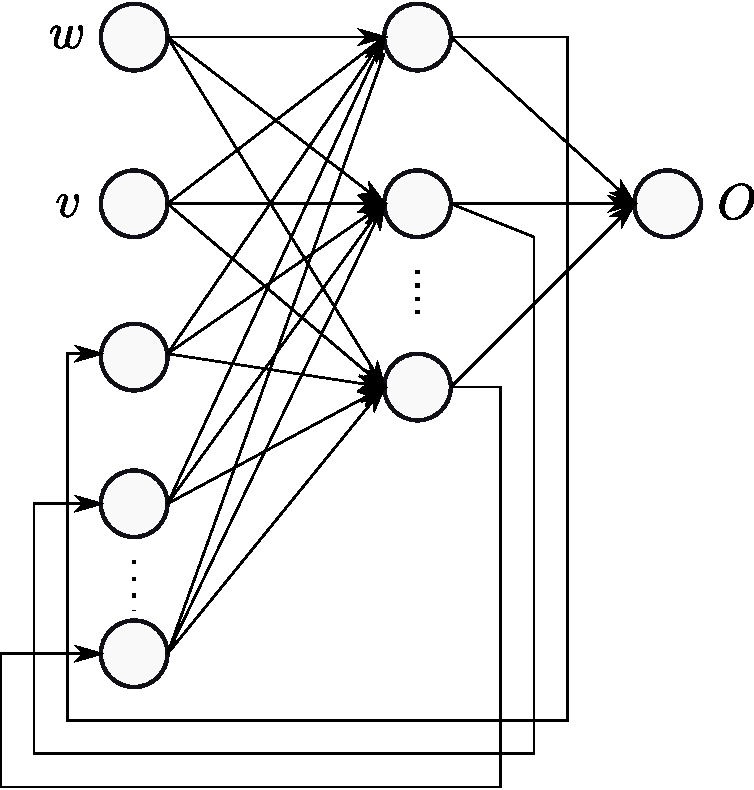
\includegraphics[width=3.0 in]{Neural_Network_CF_Swarm.pdf}
	\caption{The structure of the classifiers is a recurrent Elman neural 
    network with two inputs (agent linear speed, $v$ and angular speed, $w$), five hidden neurons, and one output neuron ($O$). $O$ is used for making a judgment. Two bias neurons (which are not shown) with a constant input of 1.0 are connected to each neuron of the hidden and output layers. See text for details.}
	\label{fig:neural_network_cf_swarm}
\end{figure}

\subsubsection{Classifiers}

The classifier can be any algorithm that takes a sequence of data about the observed individual as input, and outputs a decision (i.e., whether the observed individual is believed to be an agent or replica). 

We represent the classifier as a recurrent Elman neural network~\cite{Elman1990}. The structure of the classifier is shown in Figure~\ref{fig:neural_network_cf_swarm}. The network has $i$ inputs, $h$ hidden neurons and one output neuron. Each neuron of the hidden and output layers has a bias. The network has a total of $(i+1) h + h^2 + (h+1)$ parameters, which all assume values in $\mathbb{R}$. The activation function used in the hidden and the output neurons is the logistic sigmoid function, which has the range $\left(0,1\right)$ and is defined as: 
%
\begin{equation}\label{equ:logistic_sigmoid}
\textrm{sig}\,x = \frac{1}{1+e^{-x}}\quad\forall x \in \mathbb{R}.
\end{equation}
%
The classifier makes judgments about all individuals---both agents and replica. It observes each individual over a set period of time (i.e., a trial). The final value of its output neuron, $O$, is used to make the judgment: the classifier judges the individual to be a replica if $O<0.5$, and an agent otherwise. The classifier's memory (value of hidden neurons) is reset after each judgment.

\subsubsection{Optimization Algorithm}\label{sec:optimization_algorithm_swarm}

The optimization of models and classifiers is realized using evolutionary algorithms. In this thesis, we use a ($\mu+\lambda$) evolution strategy with self-adaptive mutation strengths~\cite{Beyer2001, Beyer2002, Eiben2003} to optimize either population. The optimization algorithm can be thought of consisting of two sub-algorithms: one for the model population, and another for the classifier population. The sub-algorithms do not interact with each other except for the fitness calculation step (described in Section~\ref{sec:fitness_calculation_swarm}). In each sub-algorithm, the value of $\mu$ and $\lambda$ is equal, which is half of the population size. The implementation of the evolutionary algorithm is detailed as follows.

In this algorithm, an individual is a 2-tuple,
$\mathbf{a}=\left(\mathbf{x},\boldsymbol{\sigma}\right)$, where $\mathbf{x\in\mathbb{R}}^n$ represents objective parameters, and $\boldsymbol{\sigma}\in \left(0,\infty\right)^n$
represents mutation strengths. The $i$-th mutation strength in $\boldsymbol{\sigma}$ corresponds to the $i$-th element in $\mathbf{x}$. 

Each generation $g$ comprises a population of $\mu$ individuals:
\begin{displaymath}
\mathcal{P}^{\left(g\right)} = \left\{\mathbf{a}_1^{\left(g\right)}, 
\mathbf{a}_2^{\left(g\right)},\dots,\mathbf{a}_{\mu}^{\left(g\right)}\right\}.
\end{displaymath}
In the population of the first generation, $\mathcal{P}^{\left(0\right)}$, all the objective parameters are initialized to $0.0$ and all the mutation strengths are initialized to $1.0$. Thereafter, in every generation $g$, the $\mu$ parent individuals are first used to create $\lambda$ offspring individuals by recombination. For the generation of each recombined individual $\mathbf{a}^{\prime\left(g\right)}_k$, $k\in\left\{1,2,\dots,\lambda\right\}$, two individuals are chosen randomly, with replacement, from the parent population: $\mathbf{a}^{\left(g\right)}_{\chi}$ and $\mathbf{a}^{\left(g\right)}_{\psi}$, where $\chi,\psi\in\left\{1,2,\dots,\mu\right\}$. The intermediate population,  $\mathcal{P}^{\prime \left(g\right)}$, is produced using discrete and intermediate recombination, which generates the objective parameters and the mutation strengths of the recombined individual, respectively:
\begin{eqnarray}
x_{k,i}^{\prime\left(g\right)} & = & x_{\chi,i}^{\left(g\right)} \textrm{\quad OR\quad} x_{\psi,i}^{\left(g\right)},\label{eq:x_recomb}\\
\sigma_{k,i}^{\prime\left(g\right)} & = & \left(\sigma_{\chi,i}^{\left(g\right)} + \sigma_{\psi,i}^{\left(g\right)}\right)/2,
\end{eqnarray}
where $i\in\left\{1,2,\dots,n\right\}$ is indexing the elements within the vectors and, in Equation~\ref{eq:x_recomb}, the selection is performed randomly and with equal probability.

Each of the $\lambda$ recombined individuals is then mutated in order to obtain the final offspring population, $\mathcal{P}^{\prime\prime \left(g\right)}$. This is done according to:
\begin{eqnarray}
\sigma_{k,i}^{\prime\prime \left(g\right)} & = & 
\sigma_{k,i}^{\prime\left(g\right)} \exp\left(\tau^{\prime} \mathcal{N}_{k}\left(0,1\right)
+ \tau \mathcal{N}_{k,i}\left(0,1\right) \right), \label{eq:sigma_mutation}\\
x_{k,i}^{\prime\prime \left(g\right)} & 
= & x_{k,i}^{\prime\left(g\right)} + \sigma_{k,i}^{\prime\prime \left(g\right)}
\mathcal{N}_{k,i} \left(0,1\right), \label{eq:x_mutation}
\end{eqnarray}
for all $\left\{k,i\right\}$, where $k\in\left\{1,2,\dots,\lambda\right\}$ is indexing the individuals within the population and $i\in\left\{1,2,\dots,n\right\}$ is indexing the elements within the vectors. Equation~\ref{eq:sigma_mutation} generates the perturbed mutation strength from the original one according to a log-normal distribution. Equation~\ref{eq:x_mutation} mutates the objective parameter according to a normal distribution having the perturbed mutation strength as its deviation. In Equation~\ref{eq:sigma_mutation}, $\mathcal{N}_{k}\left(0,1\right)$ and $\mathcal{N}_{k,i} \left(0,1\right)$ are both random numbers generated from a standard normal distribution; however, the former is generated once for each individual (i.e. for each value of $k$), while the latter is generated separately for each element within each individual (i.e. for each combination of $k$ and $i$). The parameters $\tau^{\prime}$ and $\tau$ determine the learning rates of the mutation strengths, and are set as $\tau^{\prime} = 1/2\sqrt{2n}$, $\tau = 1/2\sqrt{2\sqrt{n}}$ (similar to~\citep{Yao1999}), where $n$ corresponds to the population size.

Once the offspring population has been generated, the $\mu$ individuals with the highest fitness from the combined population, $\mathcal{P}^{\left(g\right)}\cup \mathcal{P}^{\prime\prime\left(g\right)}$ (which contains $\mu+\lambda$ individuals), are selected as the parents to form the population of the next generation, $\mathcal{P}^{\left(g+1\right)}$. Individuals with an equal fitness have an equal chance of being selected.

\subsubsection{Fitness Calculation}\label{sec:fitness_calculation_swarm}
Let the population sizes for the models and classifiers in the coevolution be $M$ and $C$, respectively. Let the number of replicas and agents in a trial be $n_r$ and $n_a$, respectively. $n_t$ trials are conducted for a model in each generation; throughout this thesis, we assume $n_t=1$.

In our thesis, whenever multiple replicas are used, each of them executes a different model. The fitness of each model in a trial is determined by each of the $C$ classifiers in the competing population. For every classifier that wrongly judges the model as an agent, the model's fitness increases by $1$. After all evaluations, the model's fitness takes a value in $\left\{0, 1, 2, \dots, C \right\}$. This value is then normalized to $[0, 1]$. 

The fitness of each classifier in a trial is determined by its judgments for the $n_r$ replicas (each executing a different model) and $n_a$ agents. For each correct judgment of the replica, the classifier's fitness increases by $\frac{1}{2 n_r}$; for each correct judgment of the agent, the classifier's fitness increases by $\frac{1}{2 n_a}$. Therefore, the fitness of each classifier in a trial is in range $[0, 1]$. $\ceil*{\frac{M}{n_r}}$ trials\footnote{We suggest choosing $n_r$ to be a factor of $M$.} are conducted in each generation, and the fitness value of each classifier is then normalized to $[0, 1]$.

\subsubsection{Termination Criterion}

%Two termination criteria could be used for the \textit{Turing Learning} method: 1) the coevolutionary algorithm runs for a fixed number of generations; 2) The fitness of the models and classifiers maintains a steady state. In this thesis, we use the first termination criteria. 
The coevolutionary algorithm stops after running for a fixed number of generations.

\subsection{Case Studies}\label{sec:case_studies_swarm_simulation}

\subsubsection{Problem Formulation}
The agents used in our case studies are embodied and move in a two-dimensional, continuous space. The agents' embodiment is based on the e-puck~\cite{e-puck}, which is a miniature, differential-wheeled robot. Figure~\ref{fig:e-puck_body} shows an e-puck robot used in the physical experiments in Chapter~\ref{ch:swarm_physical_implementation}. 

Each agent is equipped with a line-of-sight sensor that it can use to detect the item (e.g., the background, other agents or objects~\cite{Gauci2014_ijrr}, \cite{Melvin2014_aamas}) in front of it. 
%In the object clustering case study, the objects to be clustered can also be distinguished by the agents.
%In the case of object clustering, the objects are also embodied, but passive. They are of such size to be movable by a single agent. line-of-sight sensor that makes it able to distinguish between types of items in the environment (e.g., the background and other agents)

The swarm behaviors investigated in this thesis use a reactive control architecture, as found in many biological systems\footnote{\textcolor{red}{For example, researchers have found that the complex auditory orientation behavior of female crickets is derived from simple reactive motor responses to specific sound pulses~\cite{Hedwig2004}.}}. 
%In social behaviors, ants simply follow the pheromone trails when foraging~\cite{Carroll1973}. 
The motion of each agent solely depends on the state of its line-of-sight sensor ($I$). Each possible sensor state, $I\in\{0,1,\cdots,n-1\}$, is mapped onto a pair of predefined velocities for the left and right wheels, $(v_{\ell I}, v_{rI})$. $v_{\ell I}, v_{rI} \in \left[-1,1\right]$ represent the normalized left and right wheel velocities, respectively, where $1$ ($-1$) corresponds to the wheel rotating forwards (backwards) with maximum velocity. Given $n$ sensor states, any reactive behavior can thus be represented using $2n$ system parameters. In the remainder of this thesis, we describe the corresponding controllers by writing the $2n$ parameters as a tuple in the following order:
\begin{equation}\label{controller:form}
\mathbf{p} = (v_{\ell 0}, v_{r0}, v_{\ell1}, v_{r1}, \cdots, v_{\ell (n-1)}, v_{r (n-1)}).
\end{equation}

We assume that the replica has the same differential drive and line-of-sight sensor\footnote{In Section~\ref{sec:evolving_control_and_morphology_swarm_simulation}, we show that this assumption can be relaxed by also evolving some aspect of the agent's morphology.} as the agents. The system identification task is thus to infer the control parameters in Equation~\eqref{controller:form}. This explicit representation makes it possible for us to objectively measure the quality of the obtained models in the post-evaluation analysis (as discussed in the results section). To make the evolution more challenging, the search space for the algorithm in simulation is unbounded. That is, the model parameters are unconstrained, and the replica can move with arbitrary speed. 
%
\begin{figure}[!t]
	\centering
	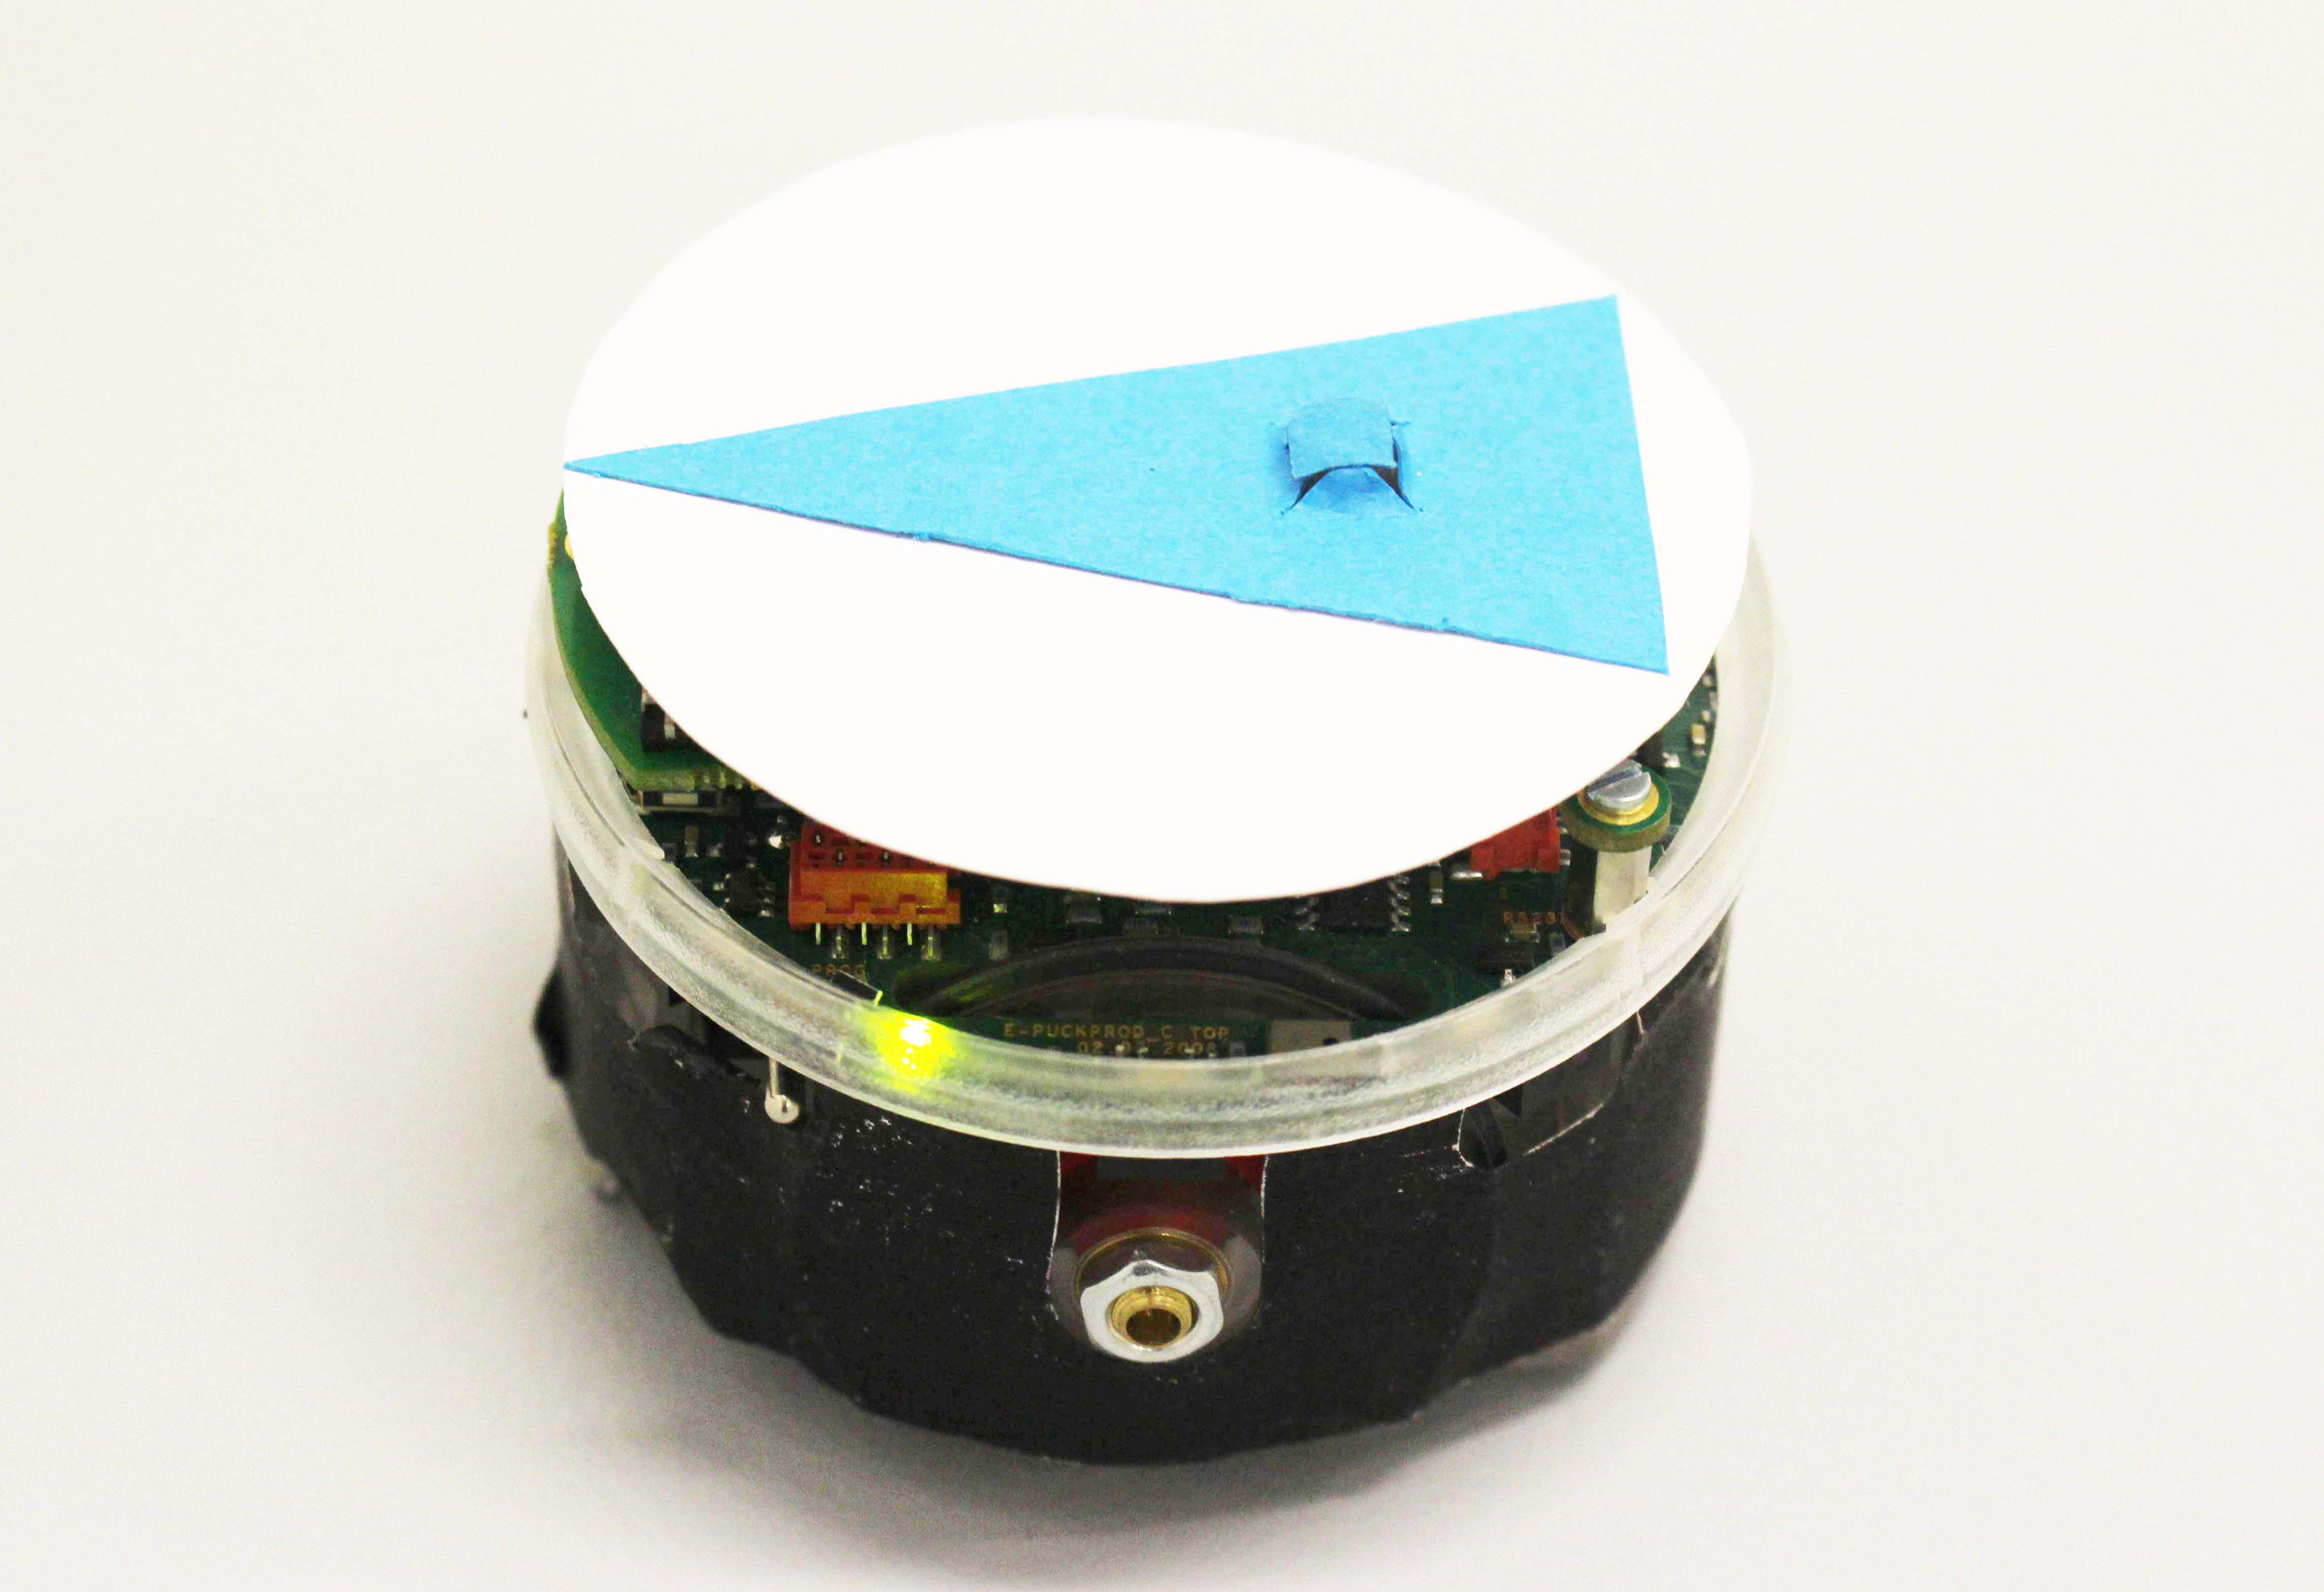
\includegraphics[width=3.5in]{e-puck_body.png}  %2.6
	\caption{An e-puck robot fitted with a black `skirt' and a top marker for motion tracking.}
	\label{fig:e-puck_body}
\end{figure}
%
\captionsetup[subfigure]{labelformat=empty}  
\begin{figure}[!t]
	\centering
	\subfloat[ \scriptsize{initial configuration}]{
		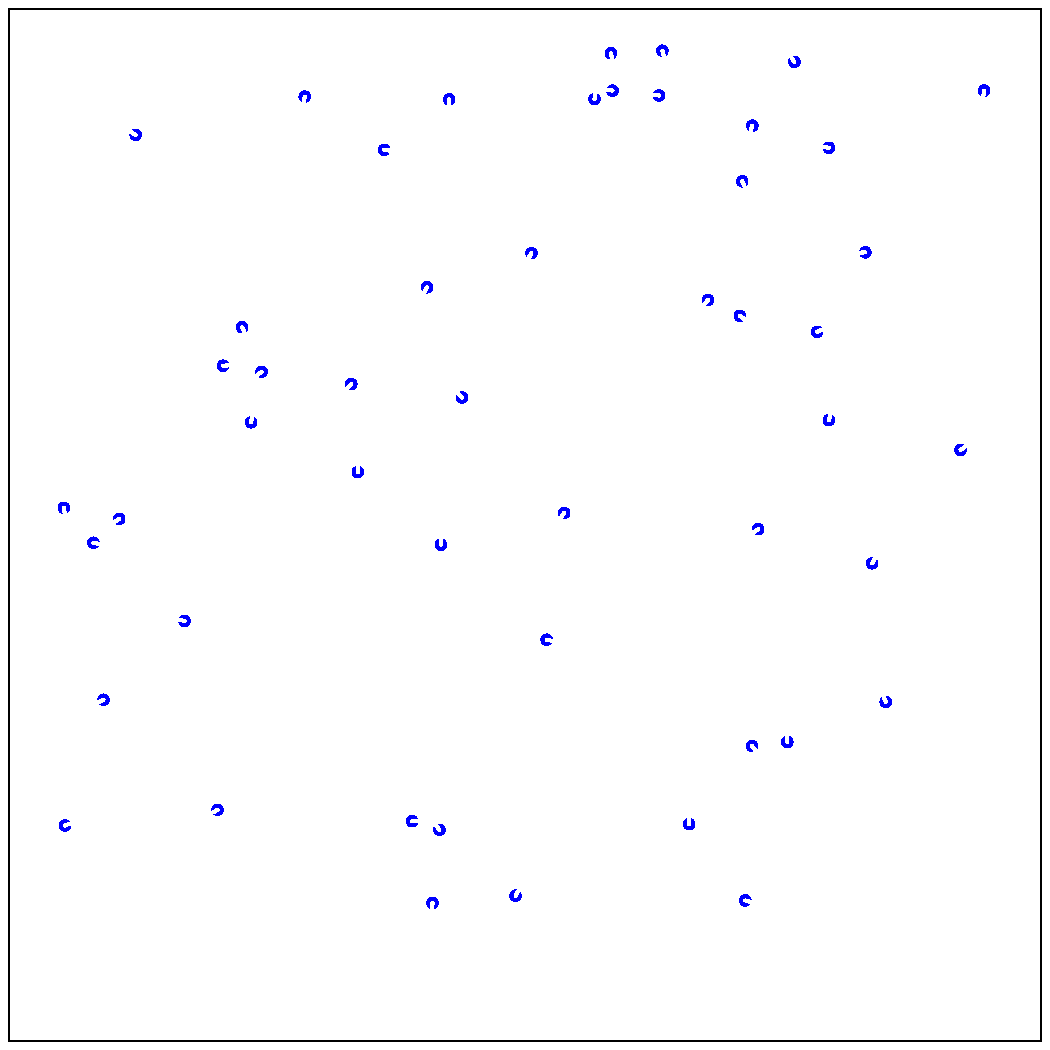
\includegraphics[width = 1.75 in]{snapshot_aggregation_initial.pdf}  %1.25
	}
	\subfloat[\scriptsize{after $60$ $\unit{s}$}]{
		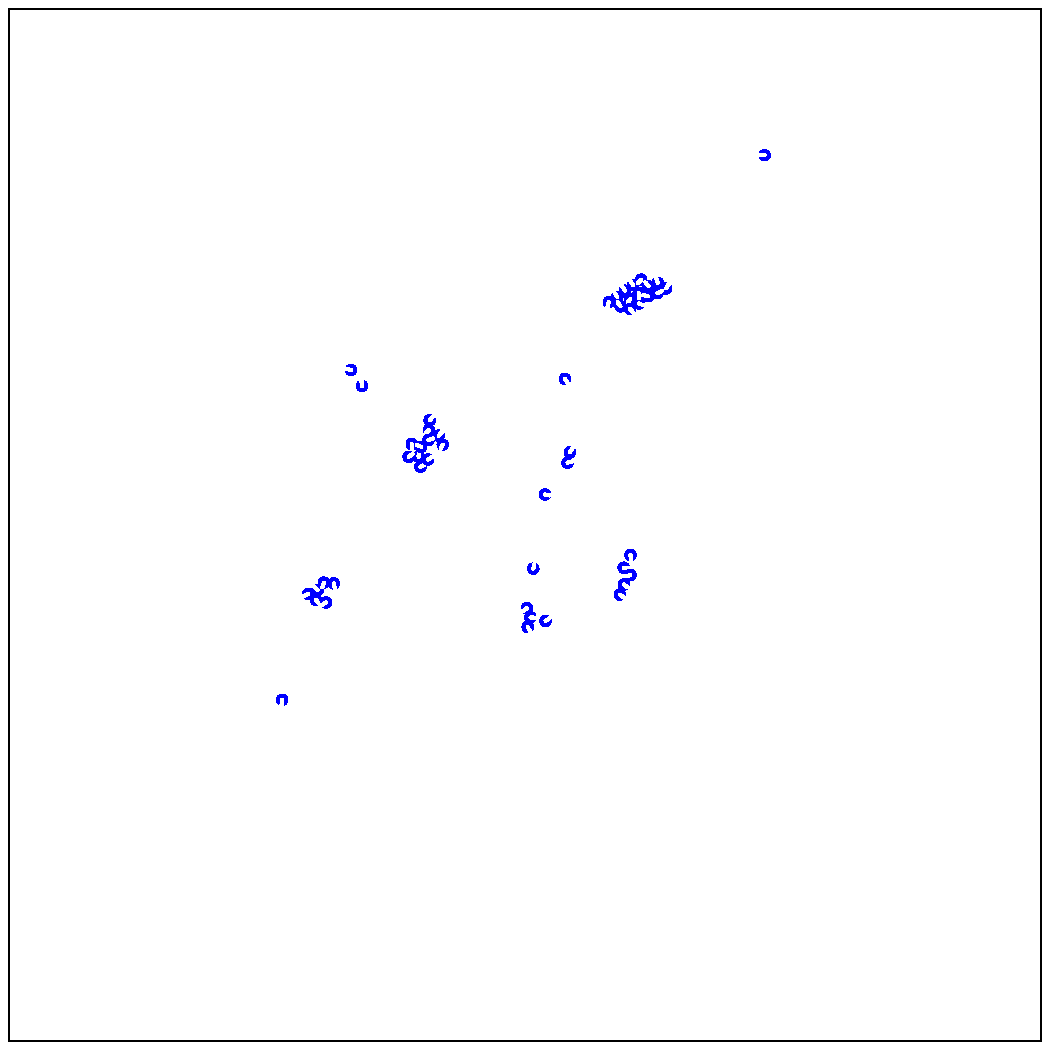
\includegraphics[width = 1.75 in]{snapshot_aggregation_60s.pdf}
	}\\
	\subfloat[\scriptsize{after $180$ $\unit{s}$}]{
		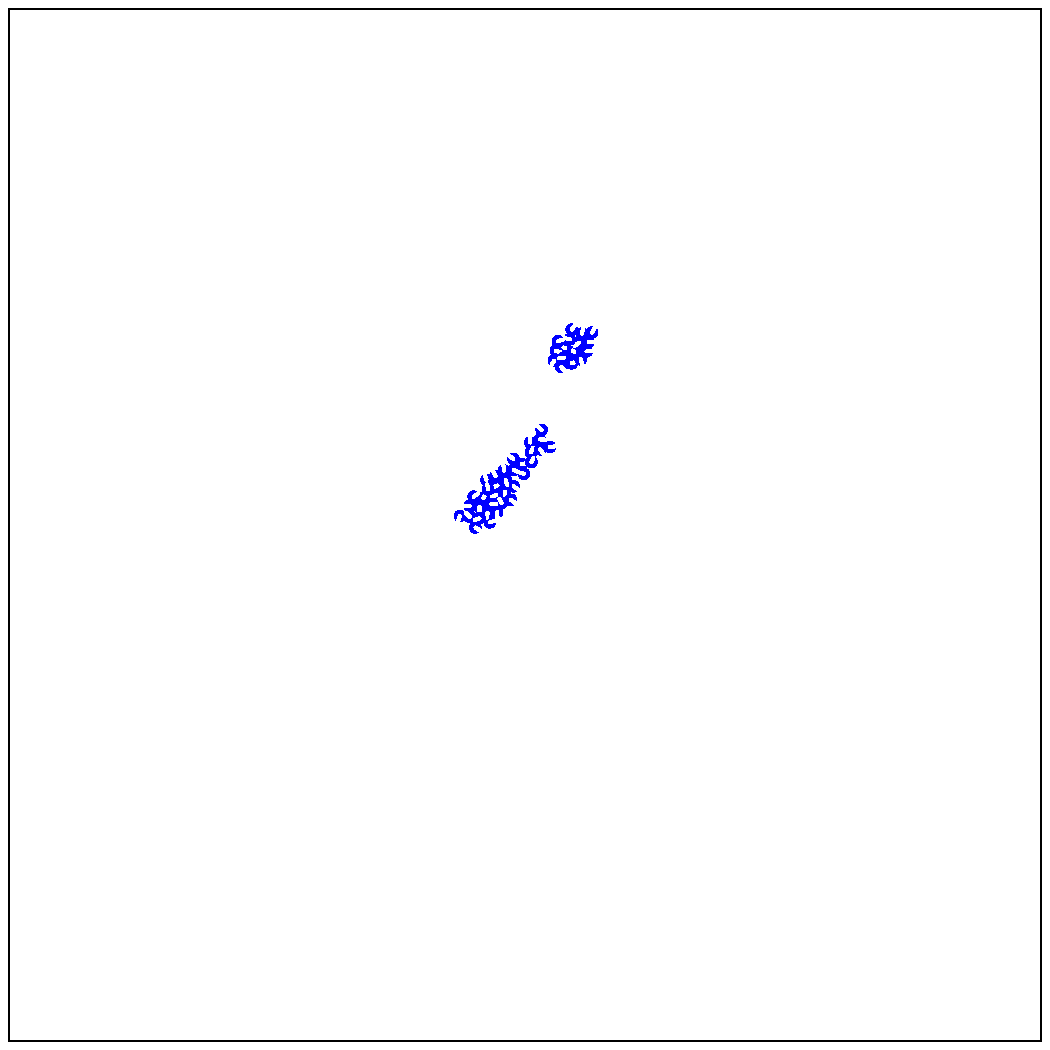
\includegraphics[width = 1.75 in]{snapshot_aggregation_180s.pdf}
	}
	\subfloat[\scriptsize{after $300$ $\unit{s}$}]{
		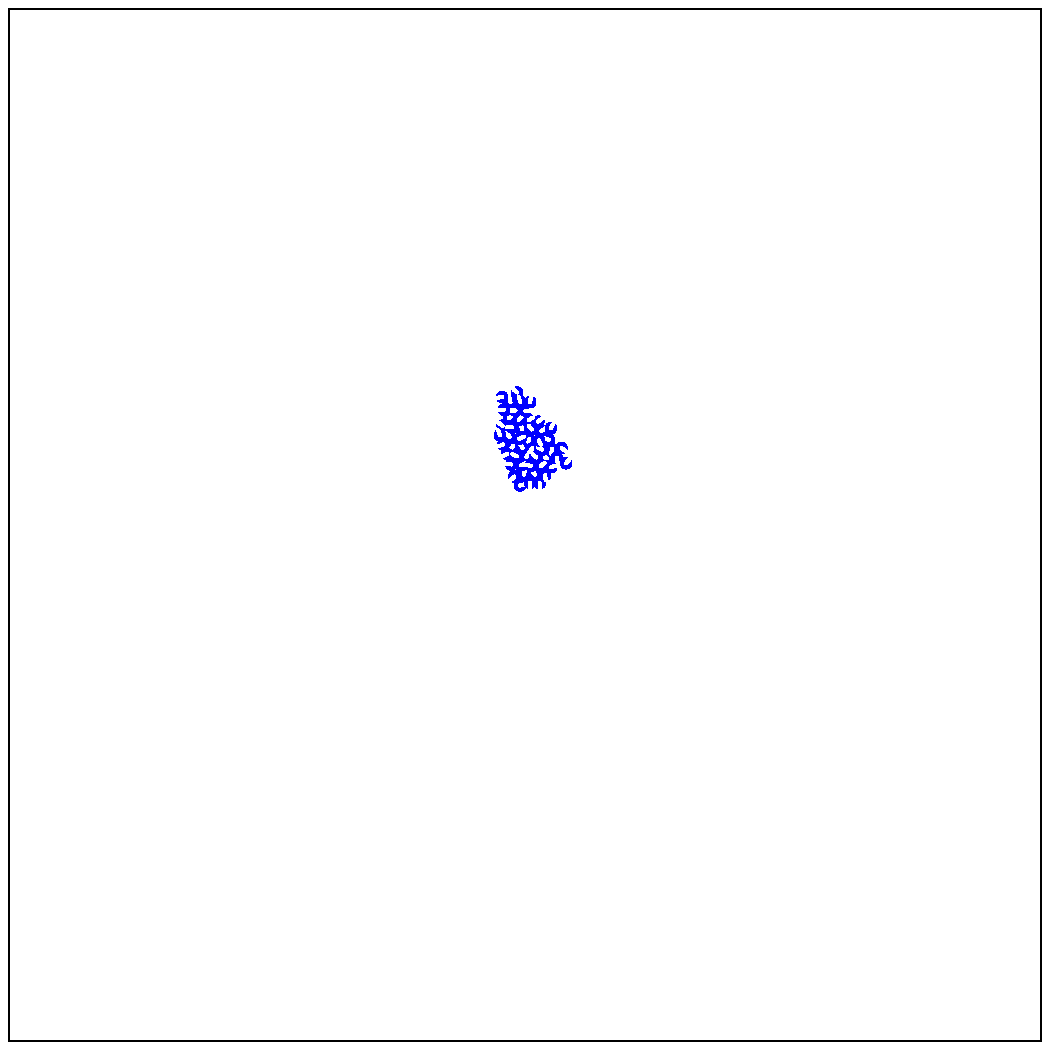
\includegraphics[width = 1.75 in]{snapshot_aggregation_300s.pdf}
	}
	\caption{Snapshots of the aggregation behavior of $50$ agents in simulation. }
	\label{fig:aggregation_snapshoot}
\end{figure}

The classifier does not have any prior knowledge about the individual under investigation. It is fed with the sequence of motion data of the individual. It has two input neurons ($i=2$), five hidden neurons ($h=5$) and one output neuron. The input neurons represent the linear speed ($v$) and angular speed ($\omega$) of the individual. They are obtained by tracking the positions and orientations of individuals. In simulation, the tracking is noise-free (situations with noise being
present are considered in Section~\ref{sec:noise_study_swarm_simulation} and the physical experiments in Chapter~\ref{ch:swarm_physical_implementation} where noise is inherently present). We define the linear speed to be positive when the angle between the individual's orientation and its direction of motion is smaller than $\unit[\pi \small/ 2]{rad}$, and negative otherwise. %This number was chosen arbitrarily and we did not attempt to optimize the number required. 

In the following, we detail the behavioral rules of the two swarm behaviors.

\captionsetup[subfigure]{labelformat=empty}  
\begin{figure}[!t]
	\centering
	\subfloat[\scriptsize{initial configuration}]
	{
		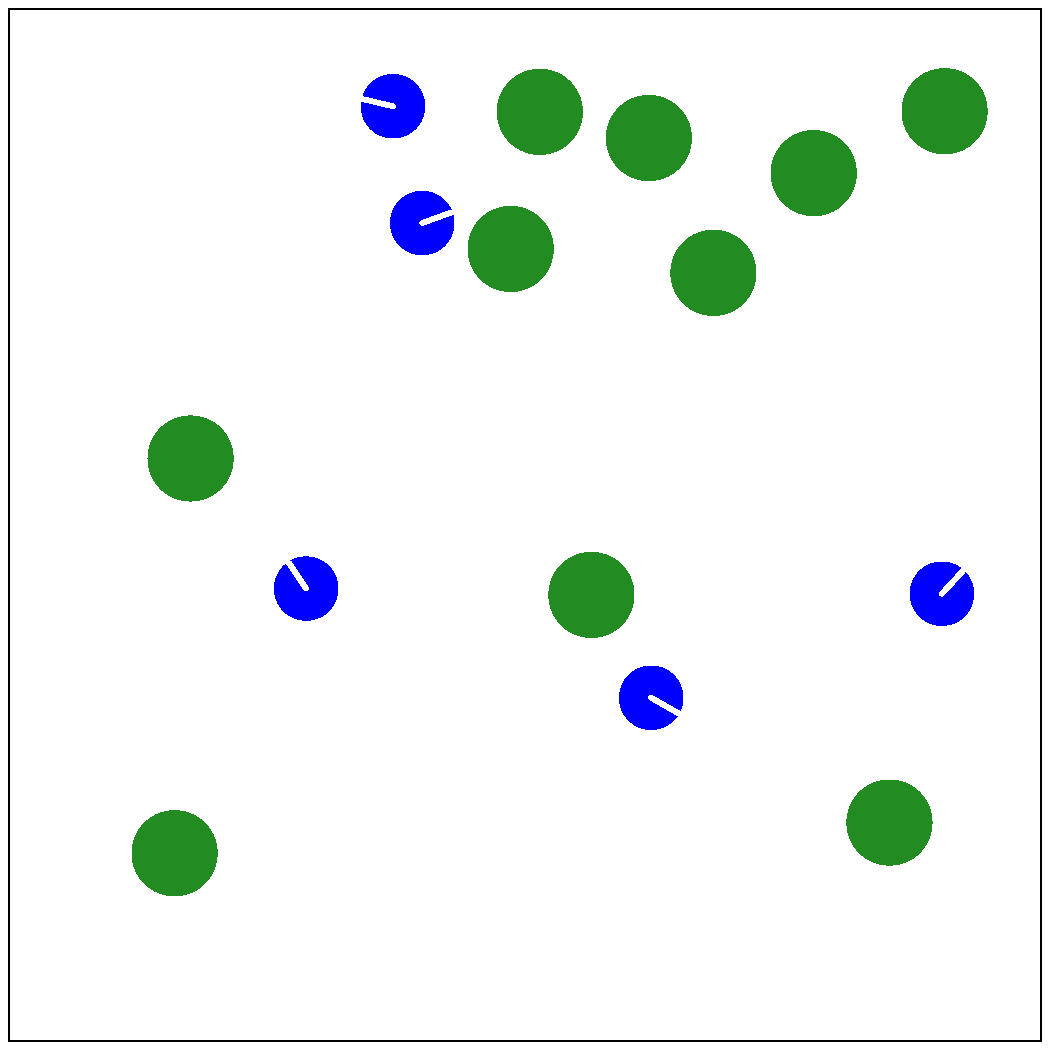
\includegraphics[width = 1.75 in]{snapshot_clustering_initial.pdf}  %1.25
	}
	\subfloat[\scriptsize{after $20$ $\unit{s}$}]{
		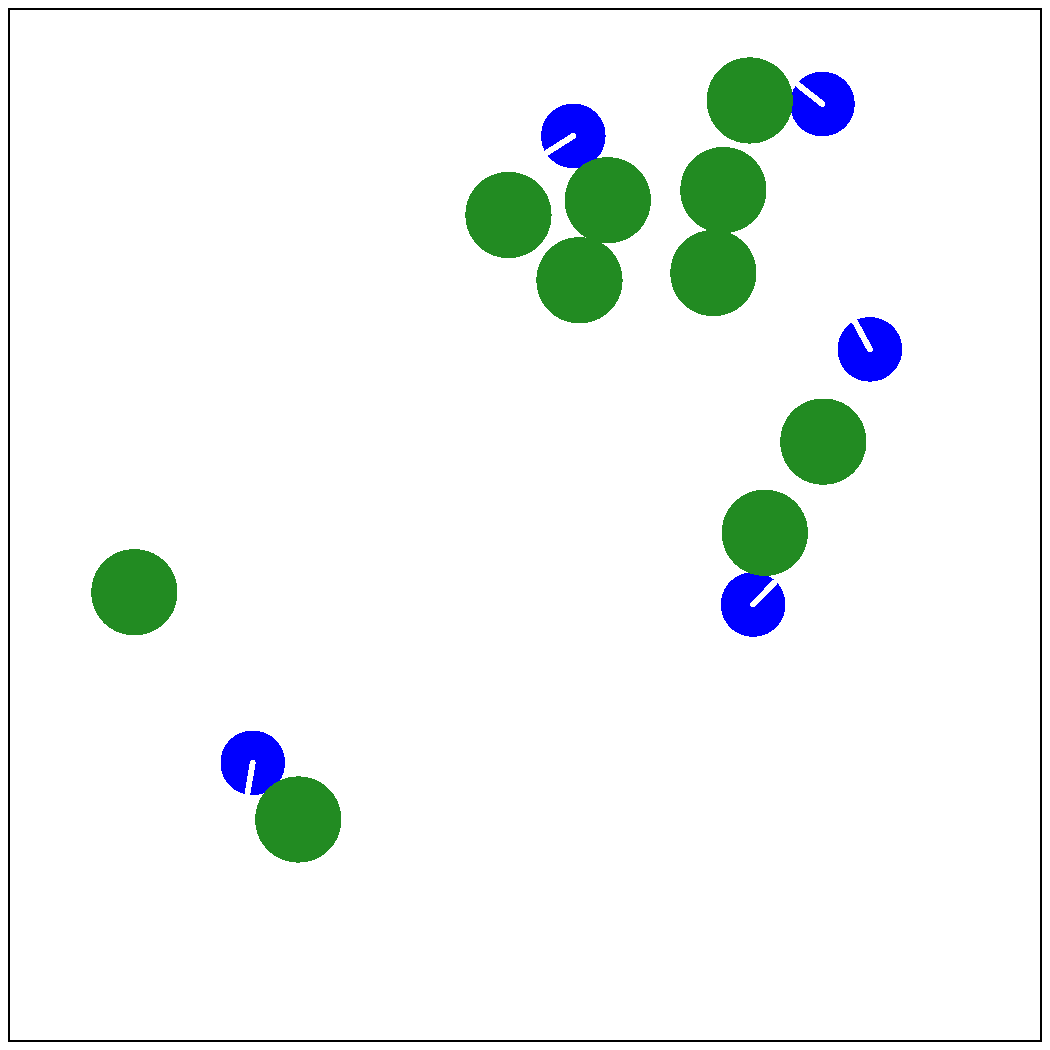
\includegraphics[width = 1.75 in]{snapshot_clustering_20s.pdf}
	}\\
	\subfloat[\scriptsize{after $40$ $\unit{s}$}]{
		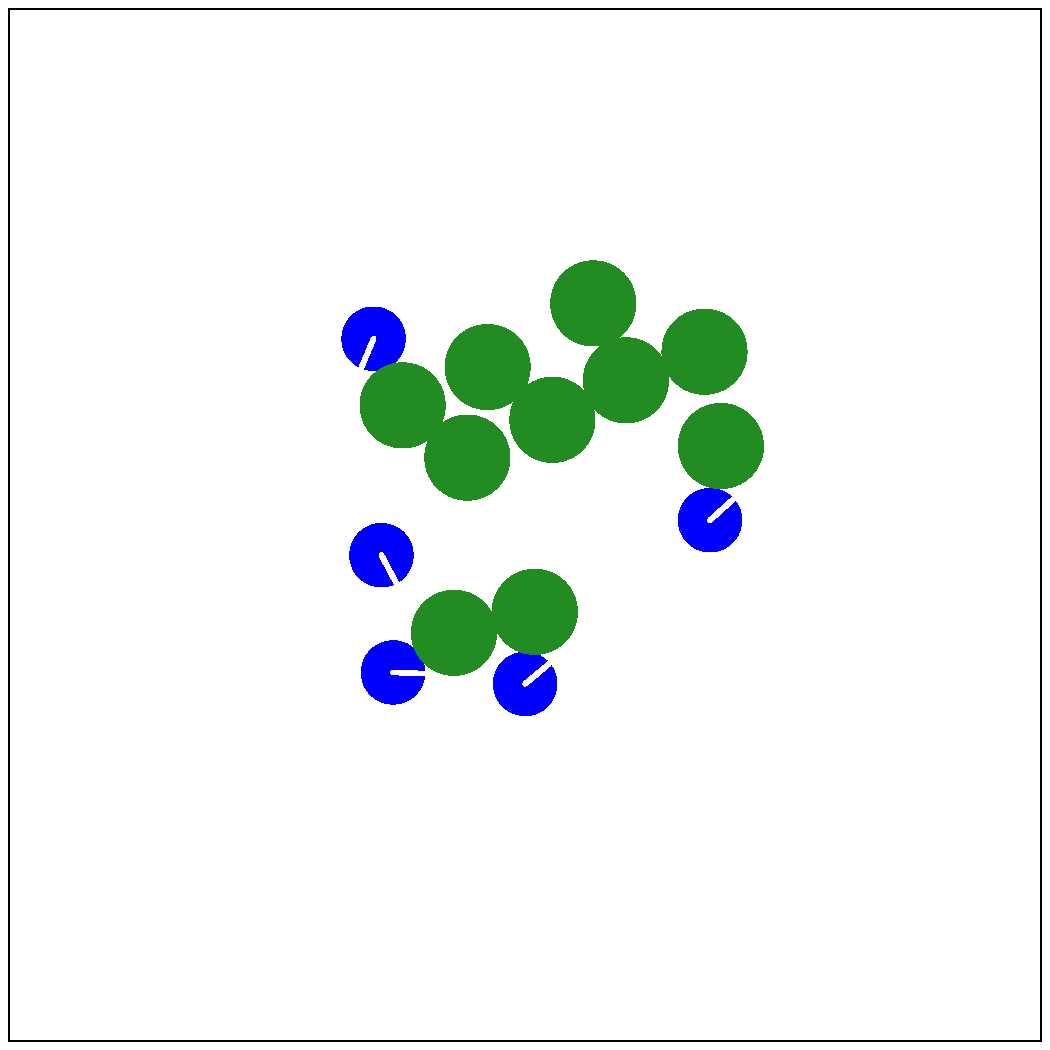
\includegraphics[width = 1.75 in]{snapshot_clustering_40s.pdf}
	}
	\subfloat[\scriptsize{after $60$ $\unit{s}$}]{
		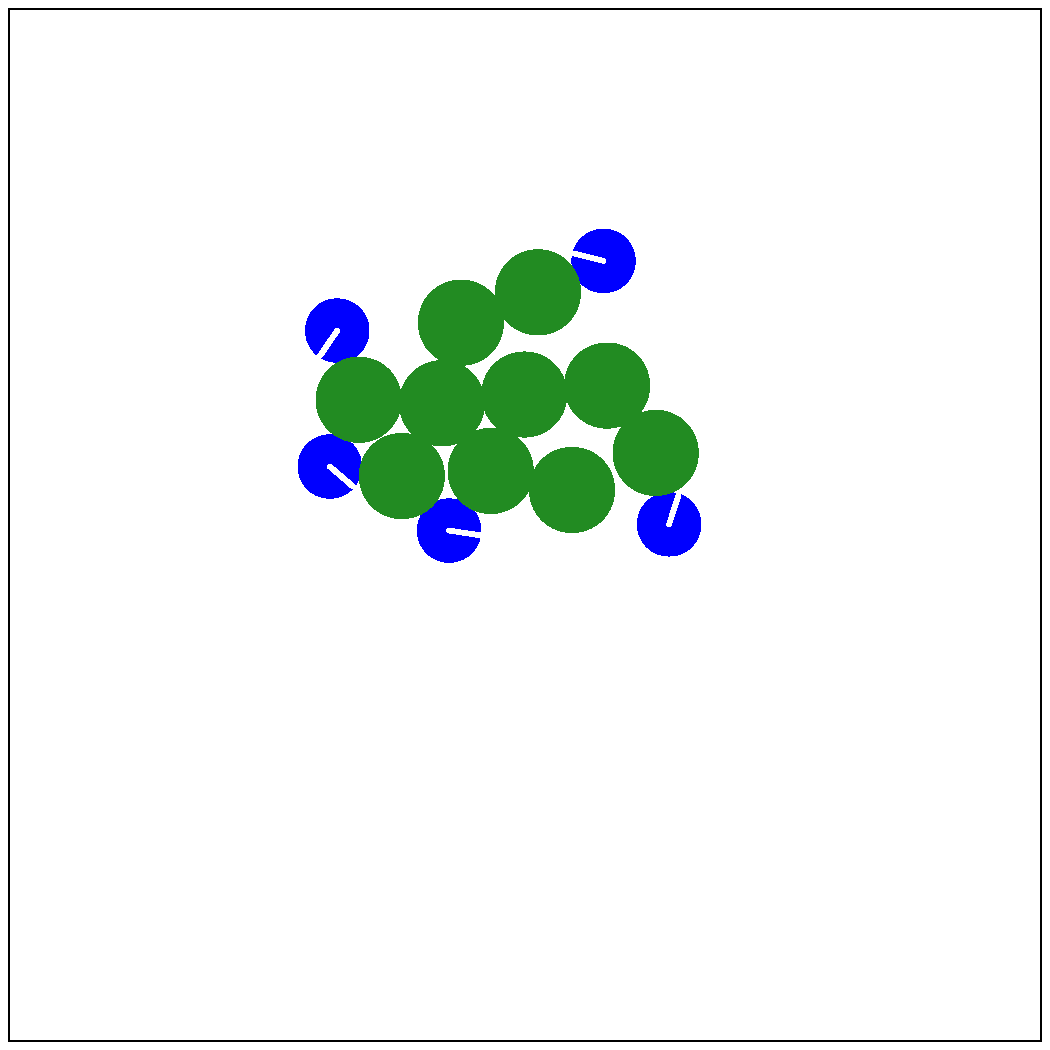
\includegraphics[width = 1.75 in]{snapshot_clustering_60s.pdf}
	}\\
	\caption{Snapshots of the object clustering behavior in simulation. There are $5$ agents (blue) and 10 objects (green).}
	\label{fig:clustering_snapshoot}
\end{figure}

\subsubsection{Aggregation}\label{sec:aggregation_behavior}
%
In this behavior, the sensor is binary, that is, $n=2$. It gives a reading of $I=1$ if there is an agent in the line of sight, and $I=0$ otherwise. The environment is free of obstacles. The objective for the agents is to aggregate into a single compact cluster as fast as possible. Further details, including a validation with 40 physical e-puck robots, are reported in~\cite{Gauci2014_ijrr}. %The agents are homogeneous: they all execute the same behavior. 

The `optimal' controller for aggregation was found by performing a grid search over the entire space of possible controllers (with finite resolution)~\cite{Gauci2014_ijrr}. The `optimal' controller's parameters are:
\begin{equation}\label{eq:aggregation_optimal_controller}
\mathbf{p} = \left(-0.7, -1.0, 1.0, -1.0\right). 
\end{equation}

When $I=0$, an agent moves backwards along a clockwise circular trajectory ($v_{\ell0} = -0.7$ and $v_{r0} = -1.0$). When $I=1$, an agent rotates clockwise on the spot with maximum angular velocity ($v_{\ell1} = 1.0$ and $v_{r1} = -1.0$). Note that rather counter-intuitively, an agent never moves forward, regardless of $I$. With this controller, an agent provably aggregates with another agent or a quasi-static cluster of agents~\cite{Gauci2014_ijrr}. Figure~\ref{fig:aggregation_snapshoot} shows snapshots from a simulation trial with $50$ agents.

\subsubsection{Object Clustering}
This behavior uses $n=3$ sensor states: $I=0$ if the sensor is pointing at the background (e.g., the wall of the environment, if the latter is bounded), $I=1$ if the sensor is pointing at an object, and $I=2$ if it is pointing at another agent. The objective of the agents is to arrange the objects into a single compact cluster as fast as possible. Details of this behavior, including a validation using 5 physical e-puck robots and 20 cylindrical objects, are presented in~\cite{Melvin2014_aamas}.

The controller's parameters, found using an evolutionary algorithm~\cite{Melvin2014_aamas}, are:
\begin{equation}\label{eq:clustering_optimal_controller}
\mathbf{p} = \left( 0.5, 1.0, 1.0, 0.5, 0.1, 0.5 \right).
\end{equation} 

When $I=0$ and $I=2$, the agent moves forward along an anti-clockwise circular trajectory, but with different linear and angular speeds. When $I=1$, it moves forward along a clockwise circular trajectory. Figure~\ref{fig:clustering_snapshoot} shows snapshots from a simulation trial with $5$ agents and $10$ objects.

\section{Simulation Platform and Setups}\label{sec:simulation_platform_setups}
 
In this section, we present the simulation experiments for the two case studies, including simulation platform, simulation setups and the results obtained. 

\subsection{Simulation Platform}\label{sec:platform_swarm_simulation}

We use the open-source Enki library~\cite{Enki}, which models the kinematics and dynamics of rigid objects, and handles collisions. Enki has a built-in 2-D model of the e-puck. The robot is represented as a disk of diameter $\unit[7.0]{cm}$ and mass $\unit[150]{g}$. The inter-wheel distance is $\unit[5.1]{cm}$. The speed of each wheel can be set independently. Enki induces noise on each wheel speed by multiplying the set value by a number in the range $(0.95, 1.05)$ chosen randomly with uniform distribution. The maximum speed of the e-puck is $\unit[12.8]{\textrm{cm/s}}$, forward or backward. The line-of-sight sensor is simulated by casting a ray from the e-puck's front and checking the first item with which it intersects (if any). The range of this sensor is unlimited in simulation. 
%Although Enki models the e-puck's real sensors, we choose to implement the line-of-sight sensor independently, for the sake of accuracy (in the physical experiments, this sensor is realized using the e-puck's camera; see Section~\ref{sec:robot_platform_sensor_implementation}).

In the object clustering case study, we model objects as disks of diameter $\unit[10]{cm}$ with mass $\unit[35]{g}$ and a coefficient of static friction with the ground of $0.58$, which makes it movable by a single e-puck.

The robot's control cycle is updated every $\unit[0.1]{s}$, and the physics is updated every $\unit[0.01]{s}$.

\subsection{Simulation Setups}\label{sec:setup_swarm_simulation}

In all simulations, we used an unbounded environment. For the aggregation case study, we used groups of $11$ individuals---$10$ agents and $1$ replica that executes a model. The initial positions of individuals were generated randomly in a square region of sides $\unit[331.66]{cm}$, following a uniform distribution (average area per individual = $\unit[10000]{cm^2}$). For the object clustering case study, we used groups of $5$ individuals---$4$ agents and $1$ replica that executes a model---and $10$ cylindrical objects. The initial positions of individuals and objects were generated randomly in a square region of sides $\unit[100]{cm}$, following a uniform distribution (average area per object = $\unit[1000]{cm^2}$). In both case studies, individual starting orientations were chosen randomly in $[-\pi,\pi]$ with uniform distribution. %The initial configuration\footnote{Throughout this paper, `initial configuration' refers to initial positions and orientations of the individuals or objects, if any.} of the individuals is randomly generated in each trial. 

We performed 30 coevolution runs for each case study. Each run lasted 1000 generations. The model and classifier populations each consisted of $100$ solutions ($\mu = 50$,  $\lambda = 50$). In each trial, classifiers observed individuals for $\unit[10]{s}$ at $\unit[0.1]{s}$ intervals ($100$ data points). 

\begin{figure}[!t]%htbp
	\centering
		\subfloat[(a) Aggregation \label{fig:model_parameters_box_aggregation}]{%
			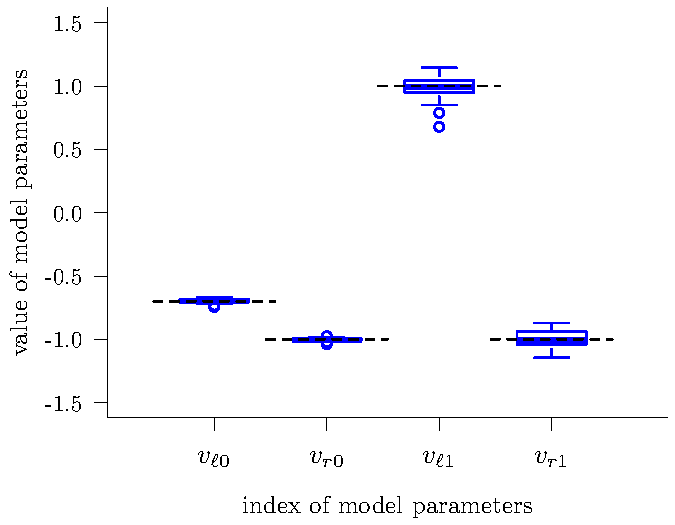
\includegraphics[width=3.0 in]{model_parameters_box_aggregation.pdf}
		}\\
		\subfloat[(b) Object Clustering\label{fig:model_parameters_box_clustering}]{%
			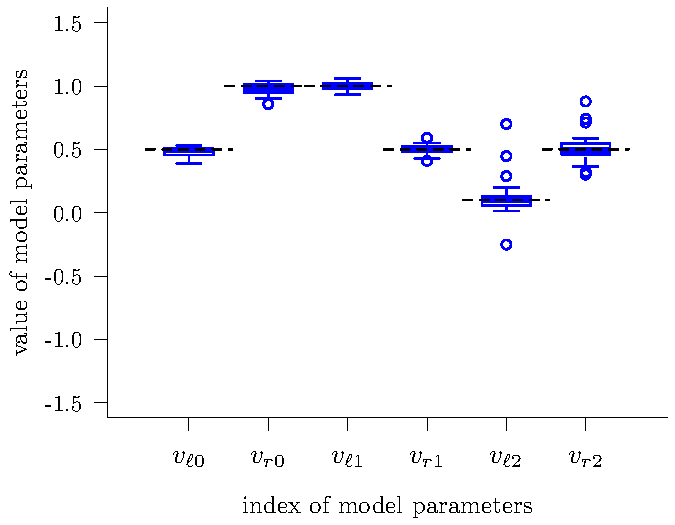
\includegraphics[width=3.0 in]{model_parameters_box_clustering.pdf}
		}
		\caption{Parameters of the evolved models with the highest subjective fitness in the $1000^\textrm{th}$ generation in the coevolutions for (a) the aggregation behavior and (b) the object clustering behavior. Each box corresponds to 30 coevolution runs in simulation. The dotted black lines correspond to the values of the parameters that the system is expected to learn (i.e., those of the agent).\label{fig:model_parameters_box}}
\end{figure}
%

\section{Simulation Results}\label{sec:results_swarm_simulation}

\subsection{Analysis of Evolved Models}\label{sec:analysis_evolved_models_swarm_simulation}

In order to objectively measure the quality of the models obtained through~\textit{Turing Learning}, we define two metrics. Given an evolved controller (model) $\mathbf{x}$ and the original agent controller $\mathbf{p}$, where $\mathbf{x},\mathbf{p}\in[-1,1]^{2n}$, we define the absolute error (AE) in a particular parameter $i\in\{1,2,\dots,2n\}$ as: 
\begin{equation}\label{eq:AE}
\mathrm{AE}_i = |x_i-p_i|. 
\end{equation}

We define the mean absolute error (MAE) over all parameters as: 
\begin{equation}\label{eq:MAE}
\mathrm{MAE} = \frac{1}{2n}\sum_{i=1}^{2n} \mathrm{AE}_i.
\end{equation}
%\footnote{Throughout the main text, we exclusively use the acronyms AE and MAE. Therefore ``mean AE'' is not to be confused with MAE; rather, it refers to the mean AE in one parameter over a number of coevolution runs.}

Fig.~\ref{fig:model_parameters_box} shows a box plot\footnote{The box plots presented here are all as follows. The line inside the box represents the median of the data. The edges of the box represent the lower and the upper quartiles of the data, whereas the whiskers represent the lowest and the highest data points that are within $1.5$ times the range from the lower and the upper quartiles, respectively. Circles represent outliers.\label{fn:boxplot}} with the parameters of the evolved models with the highest subjective fitness\footnote{The fitness of the models depends solely on the judgments of the classifiers from the competing population, and is hence referred to as \textit{subjective}.} in the final generation. It can be seen that~\textit{Turing Learning} identified the parameters for both behaviors with good accuracy (dotted black lines represent the ground truth, that is, the parameters of the observed swarming agents). In the case of aggregation, the means (standard deviations) of the AEs in the parameters were (from left to right in Fig.~\subref*{fig:model_parameters_box_aggregation}): $0.01$ ($0.01$), $0.01$ ($0.01$), $0.07$ ($0.07$) and $0.06$ ($0.04$). In the case of object clustering, these values were: $0.03$ ($0.03$), $0.04$ ($0.03$), $0.02$ ($0.02$), $0.03$ ($0.03$), $0.08$ ($0.13$) and $0.08$ ($0.09$).
%In the rest of this paper, unless otherwise stated, `evolved model' refers to the model with the highest subjective fitness in a generation.

We also investigated the evolutionary dynamics. Fig.~\ref{fig:model_parameters_convergence} shows how the model parameters converged over generations. In the aggregation case study, the parameters corresponding to $I=0$ were learned first. After around $50$ generations, both $v_{\ell0}$ and $v_{r0}$ closely approximated their true values ($-0.7$ and $-1.0$), shown in Fig.~\subref*{fig:model_parameters_convergence_aggregation}. For $I=1$, it took about $200$ generations for both $v_{\ell1}$ and $v_{r1}$ to converge. A likely reason for this effect is that an agent spends a larger proportion of its time seeing nothing ($I=0$) than other agents ($I=1$)---simulations revealed these percentages to be $91.2\%$ and $8.8\%$, respectively (mean values across $100$ trials). 

In the object clustering case study, the parameters corresponding to $I=0$ and $I=1$ were learned faster than the parameters corresponding to $I=2$, as shown in Fig.~\subref*{fig:model_parameters_convergence_clustering}. After about $200$ generations, $v_{\ell0}$, $v_{r0}$, $v_{\ell1}$ and $v_{r1}$ started to converge; however it took about $400$ generations for $v_{\ell2}$ and $v_{r2}$ to approximate their true values. Note that an agent spends the highest proportion of its time seeing nothing ($I=0$), followed by objects ($I=1$) and other agents ($I=2$)---simulations revealed these proportions to be $53.2\%$, $34.2\%$ and $12.6\%$, respectively (mean values across $100$ trials).
\begin{figure}[!t]%
	\centering
		\subfloat[(a) Aggregation \label{fig:model_parameters_convergence_aggregation}]{%
			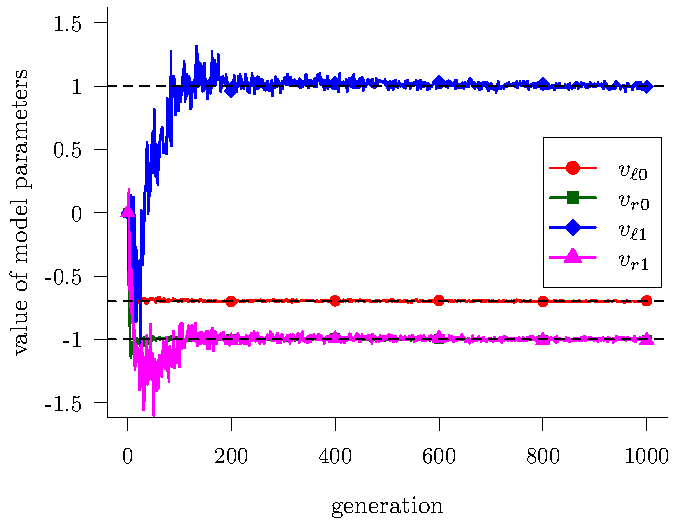
\includegraphics[width=3.0 in]{model_parameters_convergence_aggregation.pdf}
		}\\
		\subfloat[(b) Object Clustering\label{fig:model_parameters_convergence_clustering}]{%
			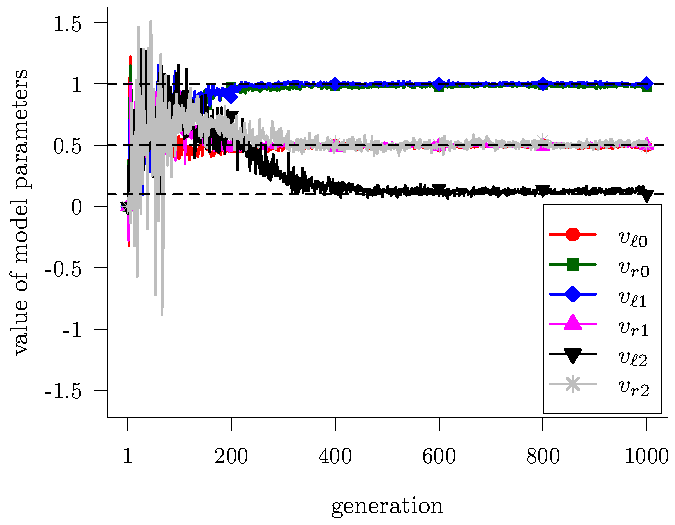
\includegraphics[width=3.0 in]{model_parameters_convergence_clustering.pdf}
		}
		\caption{Evolutionary process of the evolved model parameters for (a) the aggregation behavior and (b) the object clustering behavior. Curves represent median values across 30 coevolution runs. Dotted black lines indicate true values. \label{fig:model_parameters_convergence}}
\end{figure}

\begin{figure}[!t]
	\centering
		\subfloat[(a) Aggregation \label{fig:model_validation_aggregation_simulation}]{%
			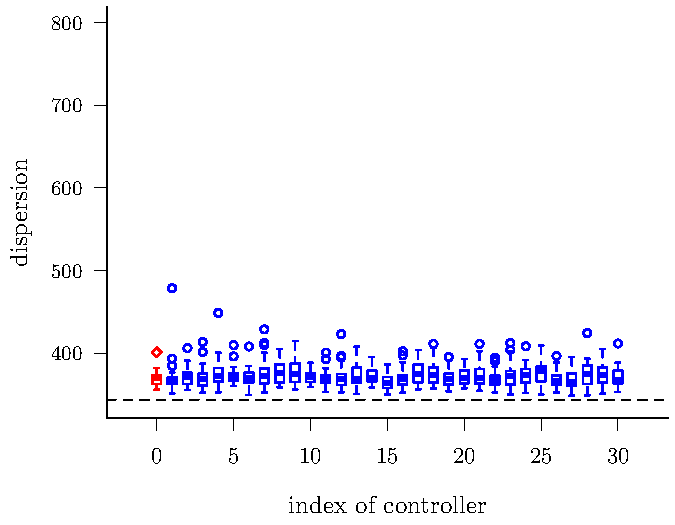
\includegraphics[width=3.0 in]{model_validation_aggregation_simulation.pdf}
		}\\
		\subfloat[(b) Object Clustering\label{fig:model_validation_clustering_simulation}]{%
			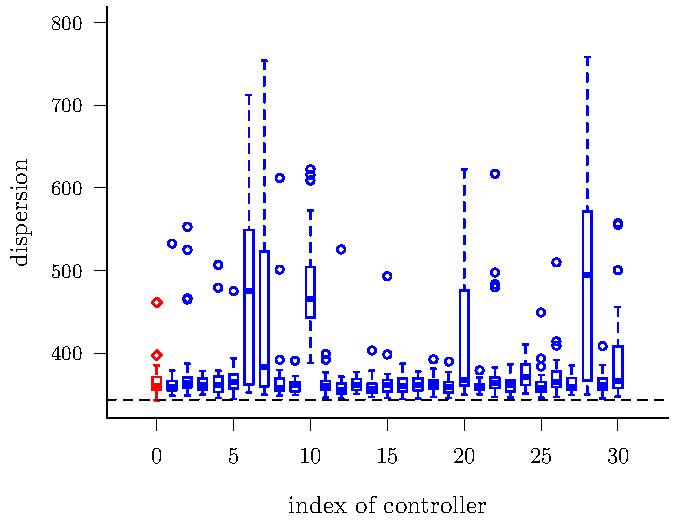
\includegraphics[width=3.0 in]{model_validation_clustering_simulation.pdf}
		}
		\caption{(a) Dispersion (after $\unit[400]{s}$) of $50$ agents executing the original aggregation controller (red box) or one of the $30$ evolved models (blue boxes) of the $1000^\mathrm{th}$ generation. (b) Dispersion (after $\unit[400]{s}$) of $50$ objects in a swarm of $25$ agents executing the original object clustering controller (red box) or one of the $30$ evolved models (blue boxes). In both (a) and (b), boxes show distributions over $30$ trials. The dotted black lines indicate the minimum dispersion that $50$ agents/objects can possible achieve~\cite{Graham1990}. See Section~\ref{sec:analysis_evolved_models_swarm_simulation} for details.\label{fig:model_validation_simulation}}
\end{figure}

Although the evolved models approximate the agents well in terms of parameters, it has often been observed in swarm systems that small changes in individual agent behaviors can lead to vastly different emergent behaviors, especially with large numbers of agents~\cite{Paul2010}. For this reason, we evaluated the quality of the emergent behaviors that the models give rise to. In the case of aggregation, a good measure of the emergent behavior is the dispersion of the swarm after some elapsed time as defined in~\cite{Gauci2014_ijrr}\footnote{The measure of dispersion is based on the robots'/objects' distances from their centroid. For a formal definition, see Equation (5) of \cite{Gauci2014_ijrr}, Equation (2) of~\cite{Melvin2014_aamas} and~\cite{Graham1990}.}. For each of the $30$ models with the highest subjective fitness in the final generation, we performed $30$ trials with $50$ agents each executing the model. For comparison, we also performed $30$ trials using the original controller (see Equation~\eqref{eq:aggregation_optimal_controller}). The set of initial configurations was the same for all models and the original controller. Fig~\subref*{fig:model_validation_aggregation_simulation} shows the dispersion for the original controller and models after $\unit[400]{s}$. All models led to aggregation. We performed a statistical test\footnote{Throughout this paper, the statistical test used is a two-sided Mann-Whitney test with a $5\%$ significance level.} on the final dispersion of the agents between the original controller and each model. There was no statistically significant difference in $26$ out of $30$ cases ($30$ out of $30$ cases with Bonferroni correction). 
%in individual agent behaviors can lead to vastly different emergent behaviors, especially with large numbers of agents~\cite{Paul2010, Luca2014}

In the case of object clustering, we use the dispersion of the objects after some elapsed time as a measure of the emergent behavior. With the original controller (see Equation~\eqref{eq:clustering_optimal_controller}) and each of the models, we performed $30$ trials with $25$ agents and $50$ objects. The results are shown in Fig.~\subref*{fig:model_validation_clustering_simulation}. In a statistical test on the final dispersion of the objects between the original controller and each model, there was no statistically significant difference in $24$ out of $30$ cases ($26$ out of $30$ cases with Bonferroni correction).

We also investigated the evolutionary process of the model parameters. Figure~\ref{fig:model_parameters_convergence} shows the convergence of the model parameters over generations. In the aggregation behavior, the parameters corresponding to $I=0$ were learned first. After about $50$ generations, both $v_{\ell0}$ and $v_{r0}$ closely approximated their true values ($-0.7$ and $-1.0$) shown in Figure~\subref*{fig:model_parameters_box_aggregation}. For $I=1$, it took about $200$ generations for both $v_{l1}$ and $v_{r1}$ to converge. A likely reason for this effect is that an agent spends a larger percentage of its time seeing nothing ($I=0$) than other agents ($I=1$)---simulations revealed these percentages to be $8.8\%$ and $91.2\%$, respectively (mean values over 100 trials). 

In the object clustering behavior, the parameters corresponding to $I=0$ and $I=1$ were learned faster than the other two parameters corresponding to $I=2$, as shown in the Figure~\subref*{fig:model_parameters_convergence_clustering}. After about $200$ generations, $v_{\ell0}$, $v_{r0}$, $v_{l1}$ and $v_{r1}$ started to converge; however it took about $400$ generations for $v_{l2}$ and $v_{r2}$ to approximate their true values. This is likely because an agent spends the most percentage of its time seeing nothing ($I=0$), followed by objects ($I=1$) and other agents ($I=2$)---simulations revealed these percentages to be $53.2\%$, $34.2\%$ and $12.6\%$ , respectively (mean values over 100 trials).

\begin{figure}[!t]%
	\centering
		\subfloat[(a) Aggregation \label{fig:fitness_curve_aggregation_simulation}]{%
			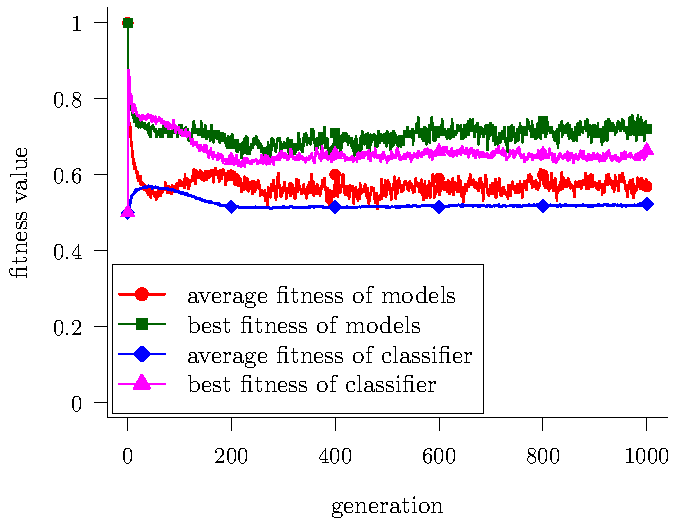
\includegraphics[width=3.5 in]{fitness_curve_aggregation_simulation.pdf}
		}\\
		\subfloat[(b) Object Clustering \label{fig:fitness_curve_clustering_simulation}]{%
			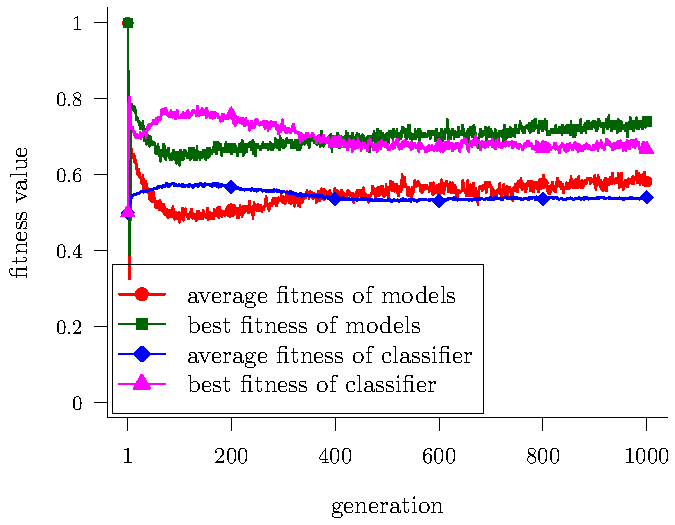
\includegraphics[width=3.5 in]{fitness_curve_clustering_simulation.pdf}
		}
		\caption{This plot shows the subjective fitness of the classifiers and
		the models for (a) the aggregation behavior and (b) the object clustering behavior.
		The curves show the median value across 30 coevolution runs.\label{fig:fitness_dynamics_simulation}}
\end{figure}

\subsection{\textcolor{red}{Coevolutionary Dynamics}}\label{sec:coevolutionary_dynamics_simulation_swarm_simulation}
In order to analyze how the classifiers and the models interact with each other during the course of the coevolution, we investigate the dynamics of the subjective fitness of the classifiers and the models as shown in Figure~\ref{fig:fitness_dynamics_simulation}. 

In the aggregation behavior, at the beginning, the fitness of the classifiers is 0.5 as they output 1 for all the agents and models, which means the classifiers make uninformed decisions\footnote{Note that in the implementation of the coevolutionary algorithm, the parameters of the models and classifiers are initialized to $0.0$, which means all the classifiers are identical at the $1^{\mathrm{st}}$ generation.}. Therefore, the fitness of the models starts from 1.0, as all the classifiers judge them the agent. Then, the average fitness of the classifiers quickly increases, corresponding to the decline of the average fitness of the models. As the models learn to adapt, the average fitness of the classifiers only increases slightly until about the $50^{\mathrm{th}}$ generation. After that, the average fitness of the models starts to increase. However, the best fitness of the classifiers is still higher than that of the models. The best fitness of the models surpasses that of the classifiers after about the $120^{\mathrm{th}}$ generation; at this point, the fitness of the `best' model (selected by the classifiers) is around $0.7$. This means that the `best' model is able to mislead $70\%$ of the classifiers into judging it as the agent. From the $200^{\mathrm{th}}$ generation onwards, the fitness of the classifiers and models remains ``balanced'' until the last generation. 

The coevolutionary dynamics of the object clustering behavior is similar. Compared with the dynamics of the aggregation behavior, it takes more generations for the fitness of the models to surpass that of the classifiers. This could be explained by the higher number of parameters and the higher complexity of the behavior to be evolved in the object clustering behavior.

\begin{figure}[!t]
	\centering
	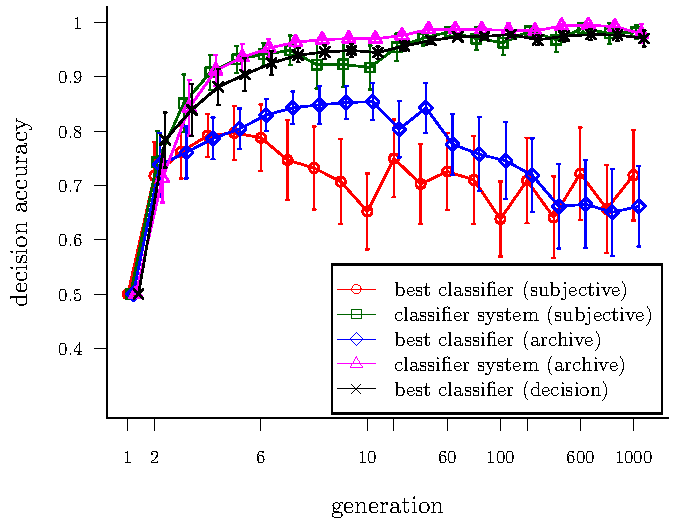
\includegraphics[width=3.0 in]{classifier_decision_accuracy_simulation.pdf}
	\caption{The average decision accuracy of the best classifiers and classifier systems over generations (nonlinear scale) in $30$ coevolution runs. The error bars show standard deviations. See text for details.}
	\label{fig:classifier_decision_accuracy_simulation}
\end{figure}

\begin{figure}[!t]%
	\centering
		\subfloat[(a) decision-making process\label{fig:classifier_output_sequence}]{%
			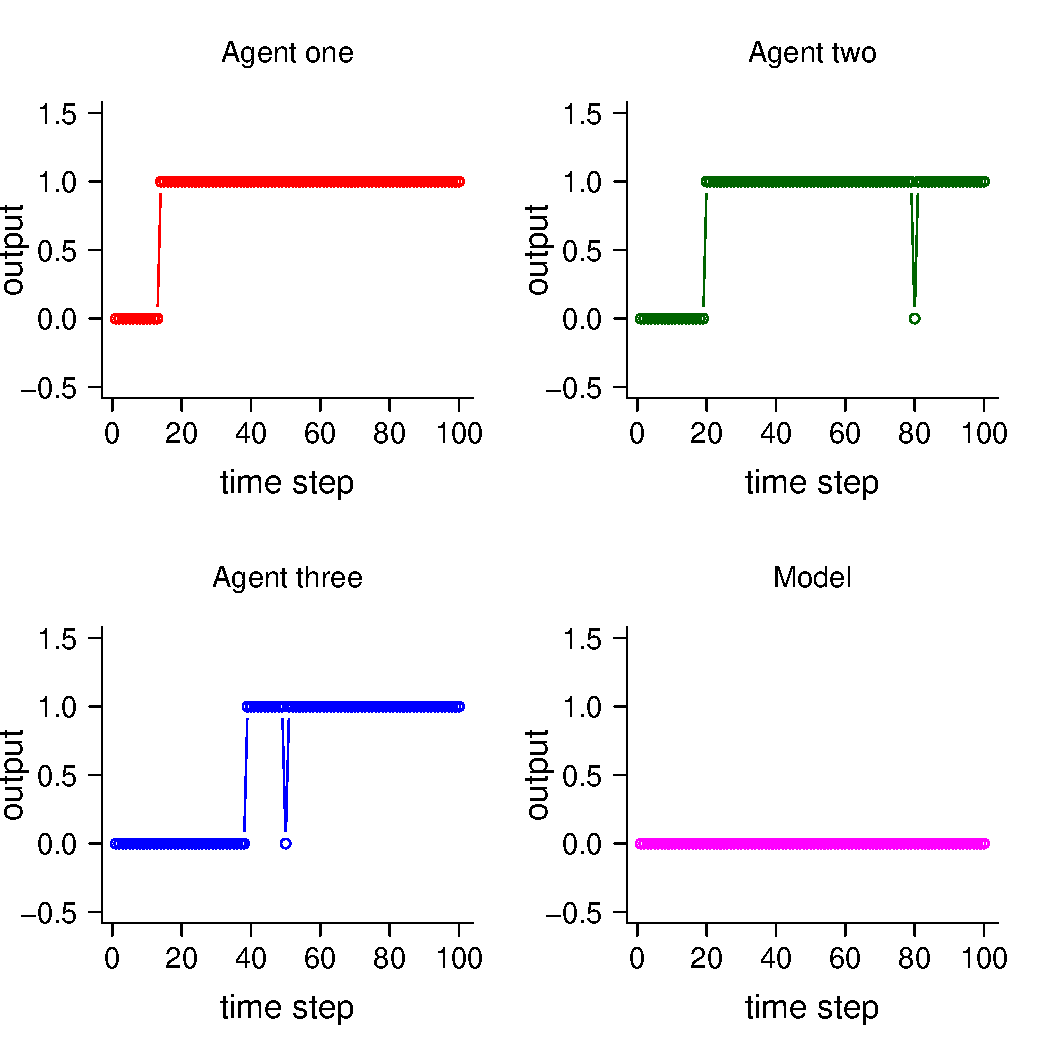
\includegraphics[width=3.0 in]{classifier_output_sequence.pdf}
		}\\
		\subfloat[(b) activation of hidden neurons\label{fig:classifier_output_hidden_neurons}]{%
			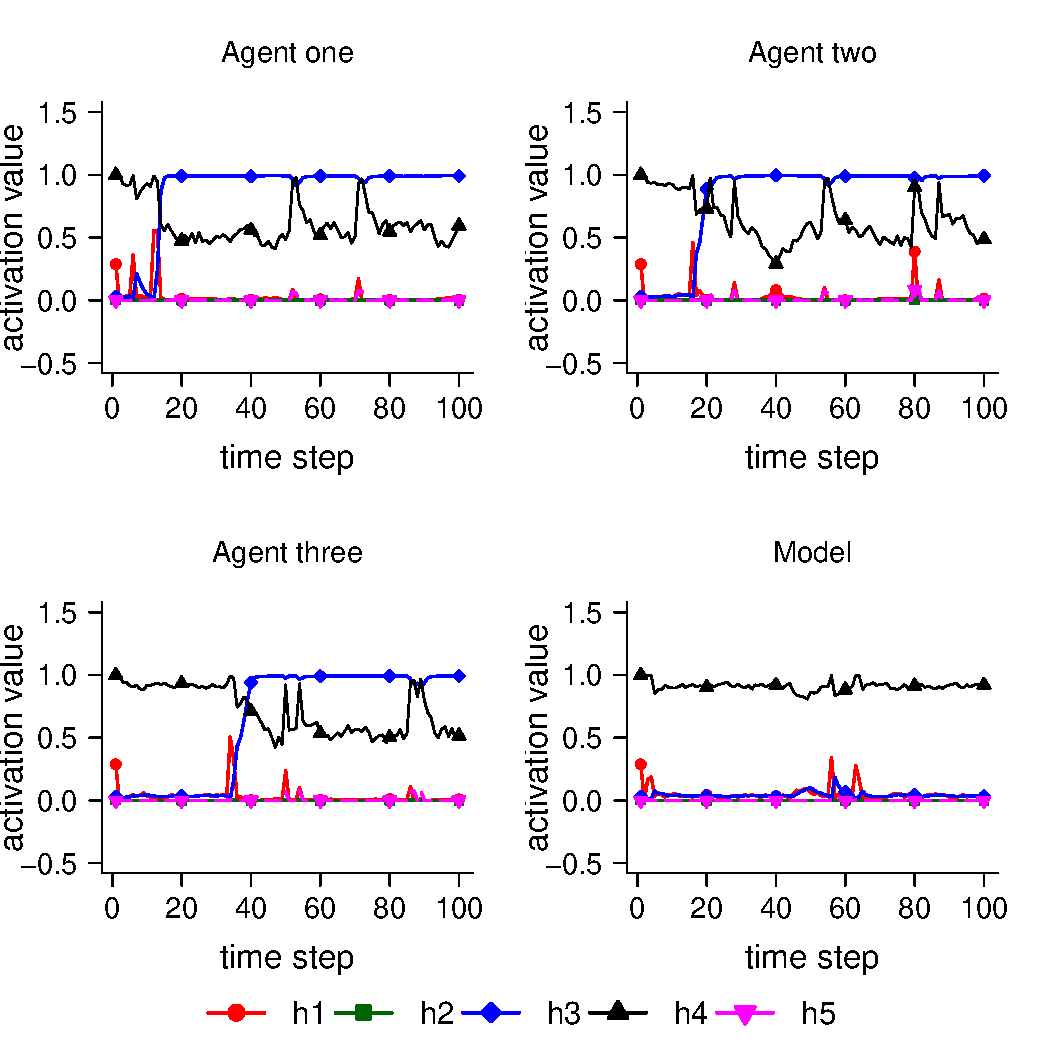
\includegraphics[width=3.0 in]{classifier_output_hidden_neurons.pdf}
		}
		\caption{This plot shows the (a) decision-making process and (b) the corresponding activation value of the $5$ hidden neurons of a classifier for three random-chosen agents and the replica that executes a very good model in a trial. Hidden neurons are labeled as $\textrm{h}1$, $\textrm{h}2$, $\textrm{h}3$, $\textrm{h}4$, and $\textrm{h}5$.}
		\label{fig:classifier_output}
\end{figure}

\subsection{Analysis of Evolved Classifiers}\label{sec:analysis_evolved_classifiers_swarm_simulation}

The primary outcome of the \textit{Turing Learning} method (and of any system identification method) is the model, which has been discussed in the previous section. However, the evolved classifiers can also be considered as a useful byproduct. For instance they could be used to detect abnormal agents in a swarm. We will now analyze the performance of the evolved classifiers. For the remainder of this paper, we consider only the aggregation case study.

To assess the performance of the classifiers, we measure the percentage of correct judgments over agents and a wide range of models. The models are uniformly distributed across the entire parameter space of the agents: $[-1,1]^4$. To keep the analysis of classifiers within a reasonable computation time, we discretize this space using $11$ settings per parameter, to obtain: $\mathcal{X} = \{-1.0, -0.8, ..., 0.8, 1.0\}^4$. This discretized space is a grid consisting of $|\mathcal{X}|=11^4=14641$ points (i.e., models). The classifier's performance is computed as follows. The model is executed by a replica mixed into a group of $10$ agents (as in the coevolution runs). $10$ trials are performed using a set of initial configurations common to all classifiers. The motion data is fed to each classifier, which makes $10$ judgments per individual. If the classifier consistently judges the individual as a model (i.e. not an agent) in $10$ out of $10$ trials, it outputs a ``model'' decision. Otherwise, it outputs ``agent''. This conservative approach was used to minimize the risk of false positive detection of abnormal behavior.

\subsubsection{Using a Single Classifier}

The average decision accuracy of the classifier with the highest subjective fitness in $30$ coevolution runs is shown in Fig.~\ref{fig:classifier_decision_accuracy_simulation} (\textit{best classifier (subjective)}). The accuracy combines the percentage of correct judgments about models ($50\%$ weight) with the percentage of correct judgments about agents ($50\%$ weight). The accuracy of the classifier increases in the first $5$ generations, then drops and fluctuates within range $62\%$--$80\%$.
%There is some fluctuation during the evolutionary process, but the accuracy is always at a low value over generations. 

An alternative strategy is to select the classifier that achieves the highest fitness when evaluated on the whole historical tracking data (not just those of the current generation). The decision accuracy of this classifier is also shown in Fig.~\ref{fig:classifier_decision_accuracy_simulation} (\textit{best classifier (archive)}). The trend is similar to that of \textit{best classifier (subjective)}. The accuracy increases in the first $10$ generations,  and then starts \emph{decaying}, dropping to around $65\%$ by the $1000^\textrm{th}$ generation. However, in the earlier generations, the accuracy of the \textit{best classifier (archive)} is higher than that of the \textit{best classifier (subjective)}. For a comparison, we also plot the highest decision accuracy that a single classifier achieves for each generation (\textit{best classifier (objective)}). Interestingly, the accuracy of the \textit{best classifier (objective)}, which is shown in  Fig.~\ref{fig:classifier_decision_accuracy_simulation} (black curve), increases almost monotonically, reaching a level above $95\%$. Note that to select the \textit{best classifier (objective)}, one needs to perform additional trials ($146410$ in this case).

At first sight, it is counter-intuitive that selecting the best classifier according to the historical data still leads to low decision accuracy. This phenomenon, however, can be explained when considering the model population. We have shown in the previous section (see especially Fig.~\subref*{fig:model_parameters_convergence_aggregation}) that the models converge rapidly at the beginning of the coevolutions. As a result, when classifiers are evaluated in later generations, the trials are likely to include models very similar to each other. Classifiers that become overspecialized to this small set of models (the ones dominating the later generations) have a higher chance of being selected in the post-evaluation. These classifiers may however have a low performance when evaluated across the entire model space.
%The selected classifiers thus become overspecialized to a small set of models: the ones dominating the later generations. 

\textcolor{red}{In order to understand how the classifiers make judgment, we analyze the internal processing through monitoring the activation of hidden neurons. Figure~\ref{fig:classifier_output} shows the decision-making process and the corresponding activation value of the $5$ hidden neurons of the classifier with the highest subjective fitness in the last generation of a coevolution run for $3$ randomly-chosen agents and the replica in a trial. The model executed on the replica has a parameter set of $(-0.7, -1.0, 1.0, -0.9)$, which is very near to that of the agent in Equation\eqref{eq:aggregation_optimal_controller}. As we can see in Figure~\subref*{fig:classifier_output_sequence}, for the agents, the classifier outputs $0$ at the beginning, and then starts to output $1$ after certain time steps, which means it needs some time to make the correct judgment. Note that for some time steps after it starts to output $1$, it still outputs $0$, but this happens only occasionally. For the model, it always outputs $0$.  This phenomenon can be explained by the activation value of the hidden neurons of the classifier in the following paragraph.}

\textcolor{red}{The classifier's activation value of the hidden neurons (labeled as $\textrm{h}1$, $\textrm{h}2$, $\textrm{h}3$, $\textrm{h}4$, and $\textrm{h}5$) shown in Figure~\subref*{fig:classifier_output_hidden_neurons} reveals its internal processing for the motion of different individuals\footnote{Note that the activation of hidden neurons may not be the same for all the classifiers due to the symmetry of neural networks, but the dynamics of each hidden neuron is similar.}. It seems that the decision-making (``sudden jump'' in Figure~\subref*{fig:classifier_output_sequence}) of the classifier is most likely related with the variation of $\textrm{h}3$ and $\textrm{h}4$. Take the agents for example, at the beginning, $\textrm{h}3$ has a very low value (which is almost $0$) and then after certain time steps it starts to increase. The variation tendency of $\textrm{h}4$ is opposite.  Every time the classifier's judgment starts to jump from $0$ to $1$, the value of $\textrm{h}3$ starts to surpass that of $\textrm{h}4$. $\textrm{h}1$, $\textrm{h}2$ and $\textrm{h}5$ are almost not activated during the whole period, although sometimes the activation of $\textrm{h}2$ influences the judgment of the classifier. For instance, there are two peaks at about $50^\textrm{th}$ and $80^\textrm{th}$ time step in $\textrm{h}2$ for agent two and three, which corresponds to a wrong judgment of the classifier (that is, it outputs $0$) at the same point. For the model, all the hidden neurons are almost not activated.}

\subsubsection{Using a Classifier System}

The results of the previous section have shown that using a single classifier is not a good solution; although there may be a good classifier in each generation, it may take significant effort (trials with agents) to find it.

To address this problem, we propose the use of a classifier system, that is, a number of classifiers working in tandem to judge a given candidate. We choose the best $10$ classifiers\footnote{Note that the number of classifiers chosen to form the system here is not necessarily optimal. \textcolor{red}{There is no guarantee that the individually best few classifiers will form the best \emph{system} when working in tandem. In principle, one could exhaustively search every possible combination of a given number of classifiers from the population. However, this is often infeasible---with our settings of choosing $10$ classifiers out of $100$, $1.73\times 10^{13}$ possibilities exist. We therefore propose the heuristic of choosing the individually best classifiers to form the system, and empirically show that this nevertheless yields good results.}}. This is either the set of $10$ classifiers with the highest subjective fitness in the current generation or the set of classifiers that achieve the highest fitness when evaluated on the whole historical data. If one or more classifiers make a decision about the candidate as a model (i.e. not an agent), the system outputs a ``model'' decision. Otherwise, it outputs ``agent''.

The results of using a classifier system are shown in Fig.~\ref{fig:classifier_decision_accuracy_simulation} (green and magenta, respectively). The two systems exhibit significantly improved decision accuracy across all generations. After $1000$ generations, each system has a high accuracy of above $95\%$, on average. 
%It seems that the classifiers in the system are complementary when making decision. 
%In stark contrast to the case of using a single classifier, 
\begin{figure}[!t]
    \centering
    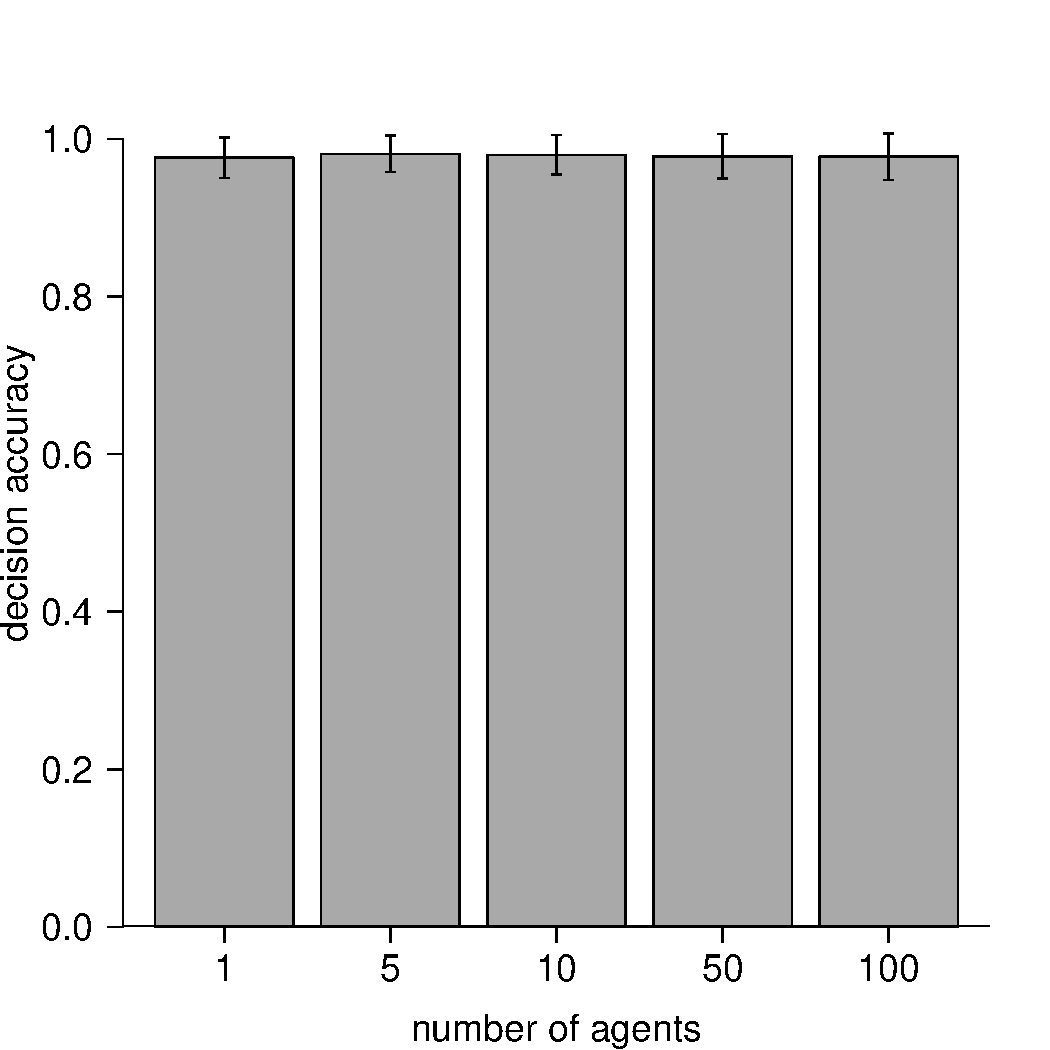
\includegraphics[width=3.5 in]{last_generation_classifier_scalability.pdf}
    \caption{\textcolor{red}{This plot shows the decision accuracy of the classifier system selected in the $1000^\mathrm{th}$ generation of $30$ coevolution runs (gray for~\textit{classifier system (archive)} and light gray for~\textit{classifier system (subjective)}) for different numbers of agents in the aggregation behavior. In each case, $14641$ different models were tested. A single replica was present in each trial.}}
    \label{fig:classifier_scalability_aggregation}
\end{figure}
%
\begin{figure}[!t]%htbp
	\centering
	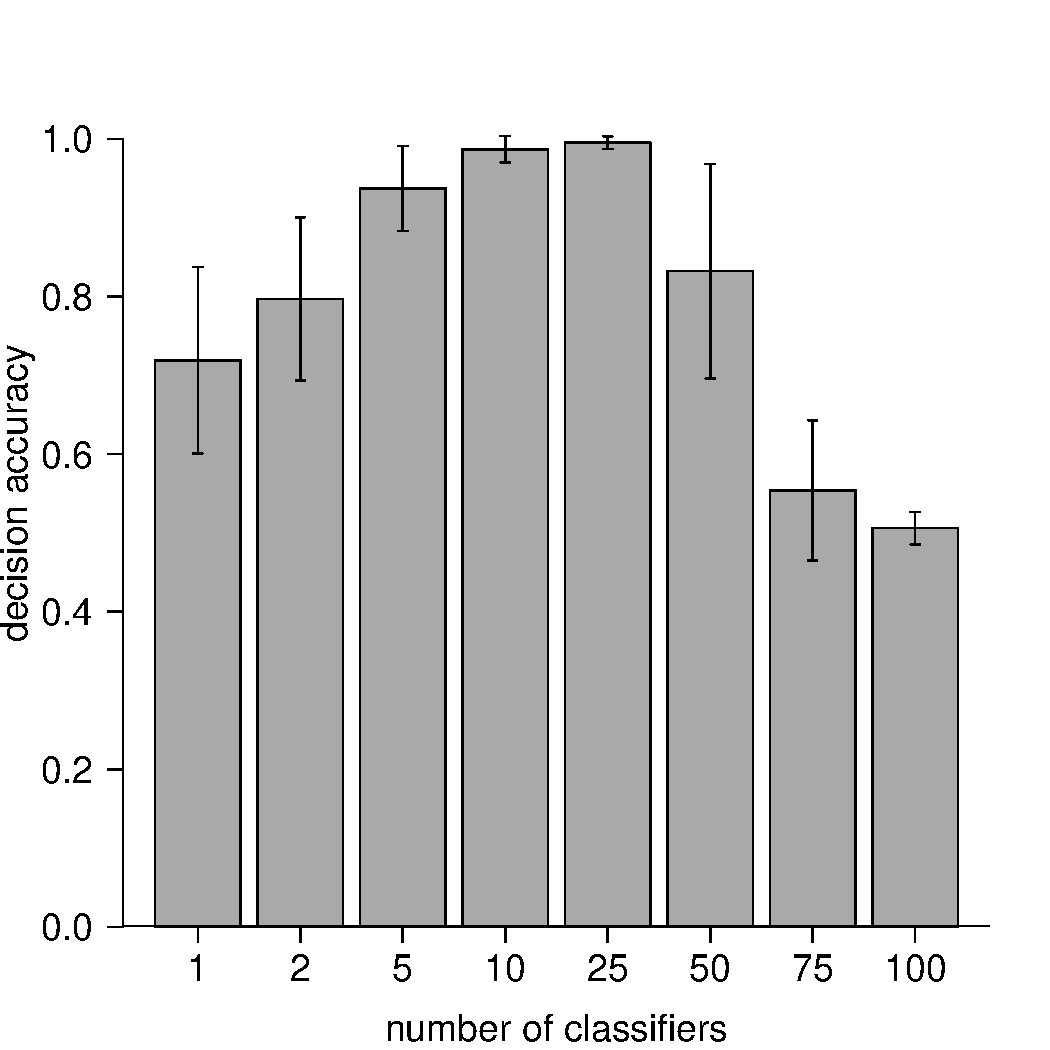
\includegraphics[width=3.5 in]{last_generation_judgment_accuracy_cf_num_selection.pdf}
	\caption{\textcolor{red}{This plot shows the decision accuracy of the classifier system in the $1000^\mathrm{th}$ generation of $30$ coevolution runs (gray for~\textit{classifier system (archive)} and light gray for~\textit{classifier system (subjective)}) with various number of classifiers chosen to form a system.}}
	\label{fig:last_generation_judgment_accuracy_cf_num_selection}
\end{figure}
%
\textcolor{red}{When post-evaluating the performance of classifier systems, we kept the setup the same as the one used in the coevolution runs. In practice, the ratio of agents and models in a trial could be different. Therefore, we analyzed the scalability of the classifier systems selected in the last generation over $30$ coevolution runs with different number of agents in the a group. Note that there is always one replica in the group. We have verified that with various number of replica in the group, similar results are obtained. We tested $14641$ different models and in each trial a model was executed on the replica. Figure~\ref{fig:classifier_scalability_aggregation} shows the decision accuracy of the classifier systems when changing the number of agents in the group. As shown in Figure~\ref{fig:classifier_scalability_aggregation}, the decision accuracy of the classifier systems is not affected by the variation of the number of agents, which shows the robustness of the classifier systems.}

\textcolor{red}{As we mentioned before, we chose $10$ classifiers to form a classifier system to have a reasonable decision accuracy, but it is heuristic. Here we investigate how the classifier system performs with various number of classifiers chosen to form a system. The decision accuracy of these classifier systems is shown in Figure~\ref{fig:last_generation_judgment_accuracy_cf_num_selection}. It seems that as long as the number of classifiers chosen to form a system is within a certain range, the system could performs well. For example, when the number of selected classifiers is between $10$ and $50$, both classifier systems can obtain a high decision accuracy. However, when the number selected classifiers is higher (e.g., $75$), the decision accuracy declines dramatically.}
%
\begin{figure}[!t]%htbp
	\centering
	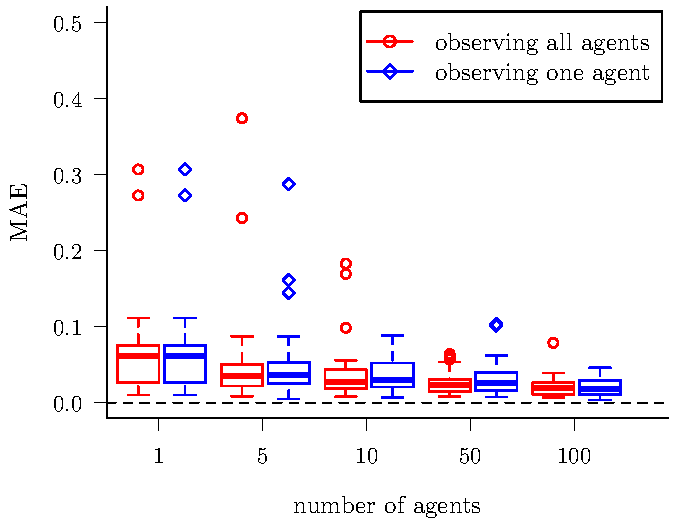
\includegraphics[width=3.0 in]{model_parameters_box_aggregation_scalability.pdf}
	\caption{MAE (defined in Equation~\eqref{eq:MAE}) of the evolved models with the highest subjective fitness after $1000$ generations, when using~\textit{Turing Learning} with varying numbers of agents (excluding the replica). Red and blue boxes show, respectively, the cases where all agents are observed, and one agent is observed. Boxes show distributions over $30$ coevolution runs. }
	\label{fig:model_parameters_box_aggregation_scalability}
\end{figure}
%
\subsection{Observing Only a Subset of Agents}\label{sec:observing_a_subset_agents_swarm_simulation}
So far, we have used motion data about all agents in the swarm when evaluating classifiers. However, this may not always be feasible in practice. For instance, given a video recording of a large and/or dense swarm, extracting motion data about all agents may be infeasible or lead to highly inaccurate results. A more practical solution might be to only track a subset of agents (e.g., by equipping them with markers).

We now compare the case where all agents are observed with the other extreme, where only one agent is observed. We study how these two cases compare as the swarm size increases. We conducted $30$ coevolution runs with each number of agents $n\in\left\{1, 5, 10, 50, 100\right\}$. There was always one replica in the group. When observing only one agent, this was chosen randomly in each trial. Note that the total number of trials in each coevolution run for the case of observing all agents and one agent is identical. We measured the total square error of the model with the highest subjective fitness in the last ($1000^\textrm{th}$) generation of each run. The results are shown in Fig.~\ref{fig:model_parameters_box_aggregation_scalability}.

There is no statistically significant difference for any $n$. On the other hand, as the swarm size increases, performance improves. For example, there is a statistically significant difference between $n=10$ and $n=100$, both when observing all agents and one. These results suggest that the key factor in the coevolutionary process is not the number of observed agents, so much as the richness of information that comes from increasing inter-agent interactions, and is reflected in each agent's motion. This means that in practice, observing a single agent is sufficient to infer accurate models, as long as the swarm size is sufficiently large.

A similar phenomenon was observed in a different scenario, where the goal was to distinguish between different `modes' of a swarm (i.e., global behaviors) through observing only a few individuals~\cite{Daniel2014}.

\begin{figure}[!t]%
	\centering
		\subfloat[(a) \label{fig:Angle_I=0}]{%
			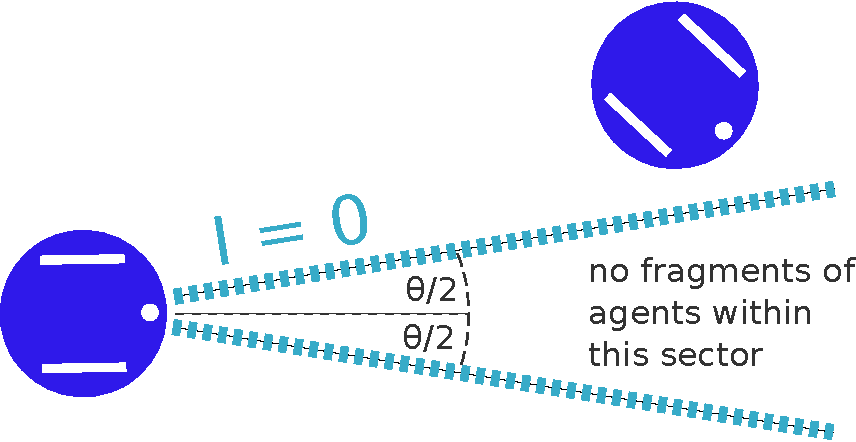
\includegraphics[width=2.2 in]{Angle_I=0.pdf}
		}\\
		\subfloat[(b) \label{fig:Angle_I=1}]{%
			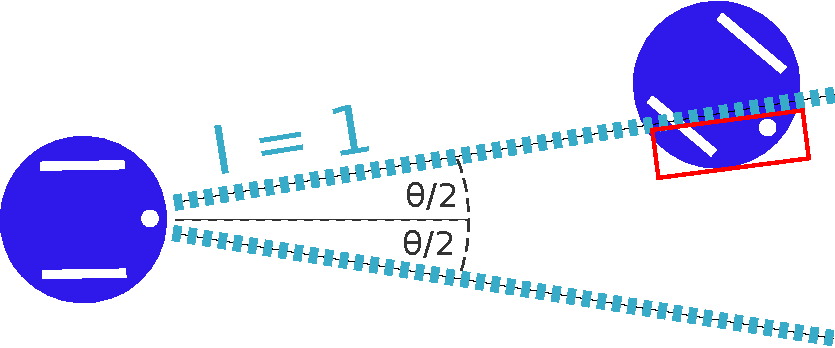
\includegraphics[width=2.2 in]{Angle_I=1.pdf}
		}
		\caption{A diagram showing the angle of view of the agent's sensor investigated in Section~\ref{sec:evolving_control_and_morphology_swarm_simulation}.}
		\label{fig:Angle_I}
\end{figure}

\begin{figure}[!t]%
	\centering
		\subfloat[(a) \label{fig:model_parameters_box_aggregation_0degree}]{%
			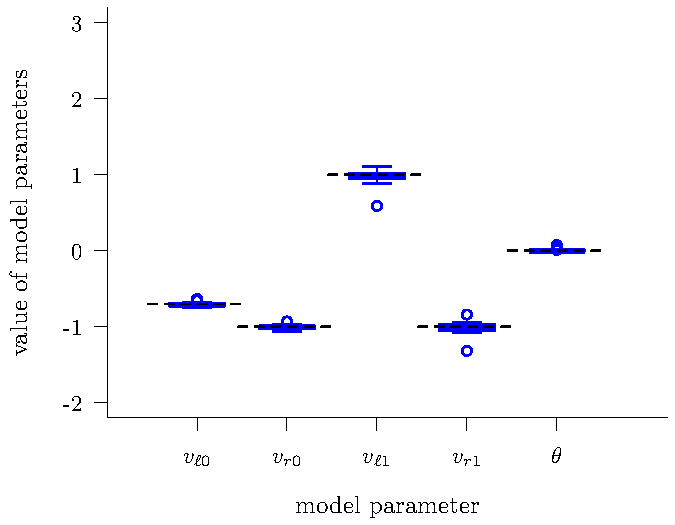
\includegraphics[width=3.5 in]{model_parameters_box_aggregation_0degree.pdf}
		}\\
		\subfloat[(b) \label{fig:model_parameters_box_aggregation_60degree}]{%
			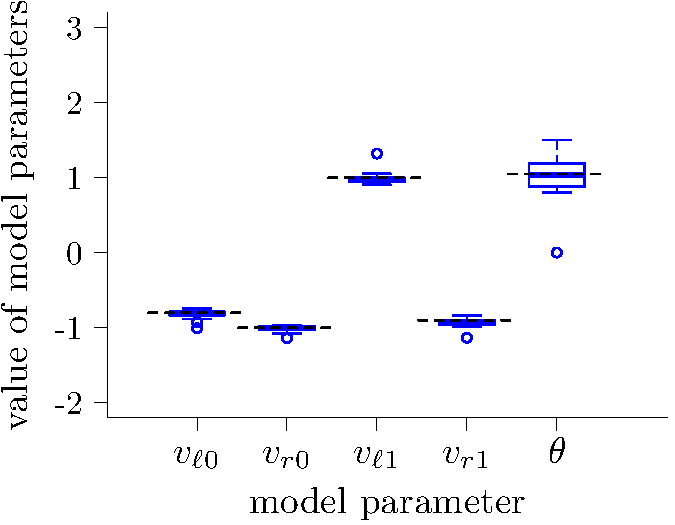
\includegraphics[width=3.5 in]{model_parameters_box_aggregation_60degree.pdf}
		}
		\caption{Parameters (controller parameters and angle of view in $\unit[]{rad}$) of the evolved models with the highest subjective fitness in the $1000^\textrm{th}$ generation corresponding to the case of the agents' angle of view equal to (a) $\unit[0]{rad}$ and (b) $\unit[\pi/3]{rad}$. Boxes show distributions over $30$ coevolution runs. Dotted black lines indicate true values.}
		\label{fig:model_parameters_box_aggregation_angle}
\end{figure}

\begin{figure}[!t]%
	\centering
		\subfloat[(a) \label{fig:model_parameters_convergence_aggregation_0degree}]{%
			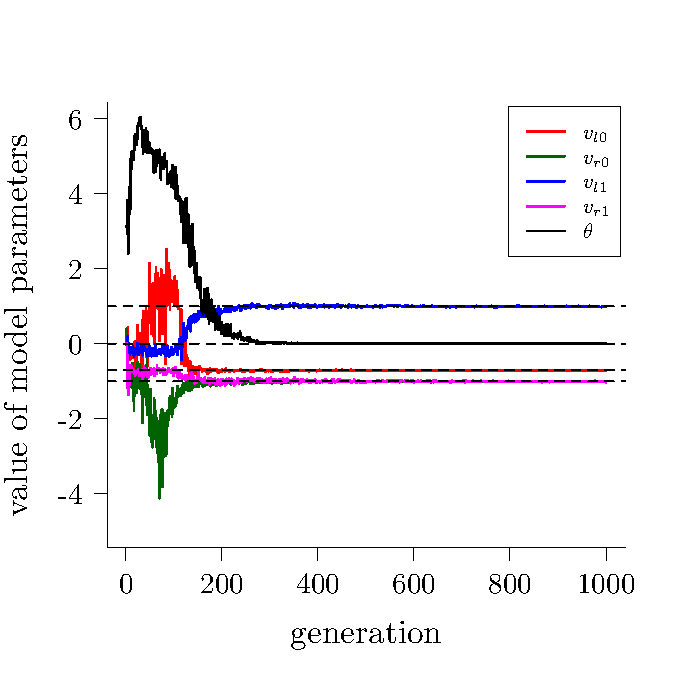
\includegraphics[width=3.5 in]{model_parameters_convergence_aggregation_0degree.pdf}
		}\\
		\subfloat[(b) \label{fig:model_parameters_convergence_aggregation_60degree}]{%
			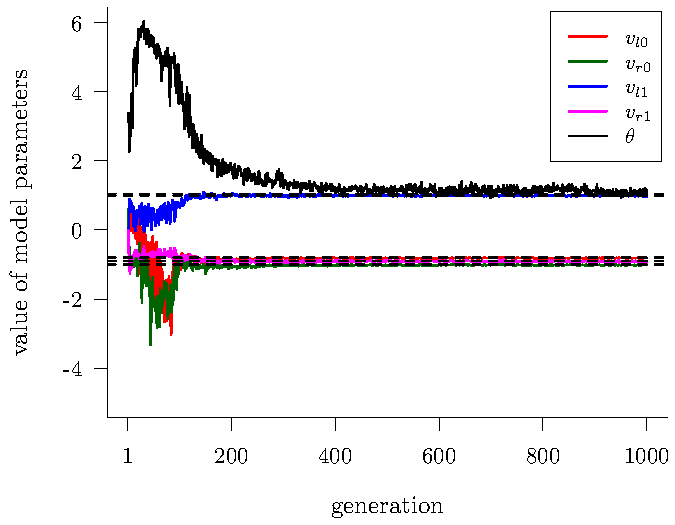
\includegraphics[width=3.5 in]{model_parameters_convergence_aggregation_60degree.pdf}
		}
		\caption{Evolutionary process of the evolved models (controller parameters and angle of view in $\unit[]{rad}$) in the $1000^\textrm{th}$ generation corresponding to the case of the agents' angle of view equal to (a) $\unit[0]{rad}$ and (b) $\unit[\pi/3]{rad}$. Boxes show distributions over $30$ coevolution runs. Dotted black lines indicate true values.. \label{fig:model_parameters_convergence_angleview}}
\end{figure}
%
\subsection{Evolving Control and Morphology}\label{sec:evolving_control_and_morphology_swarm_simulation}
In the previous sections, we assumed that we fully knew the agents' morphology (i.e., structure), and only their behavior (controller) was to be identified. We now present a variation where one aspect of the morphology is also unknown. The replica, in addition to the four controller parameters, takes a parameter $\theta\in\left[0,2\pi\right]\unit{rad}$, which determines the horizontal field of view of its sensor, as shown in Fig.~\ref{fig:Angle_I} (however, the sensor is still binary). Note that in the previous sections the agents' line-of-sight sensor can be considered as a sensor with angle of view of $\unit[0]{rad}$.

The models now have five parameters. As before, we let the coevolution run in an unbounded search space (i.e., now, $\mathbb{R}^5$). However, as $\theta$ is necessarily bounded, before a model was executed on a replica, the parameter corresponding to $\theta$ was mapped to the range $[0, 2\pi]$ using a logistic sigmoid function (Equation~\eqref{equ:logistic_sigmoid}). The controller parameters were directly passed to the replica. In this setup, the classifiers observed the individuals for $\unit[100]{s}$ in each trial (preliminary results indicated that this setup requires a longer observation time). 

Fig.~\subref*{fig:model_parameters_box_aggregation_0degree} shows the parameters of the subjectively best models in the last ($1000^\textrm{th}$) generations of $30$ coevolution runs. The means (standard deviations) of the AEs in each model parameter were: $0.02$ ($0.01$), $0.02$ ($0.02$), $0.05$ ($0.07$), $0.06$ ($0.06$) and $0.01$ ($0.01$). All parameters including $\theta$ were still learned with high accuracy.

The case where the true value of $\theta$ is $\unit[0]{rad}$ is an edge case, because given an arbitrarily small $\epsilon>0$, the logistic sigmoid function maps an infinite domain of values onto $(0,\epsilon]$. 
%(i.e., $\forall\epsilon>0.\, \exists x_0.\, \forall x<x_0.\, \textrm{sig}\,x < \epsilon $). 
This makes it easier for the coevolution to learn this parameter. For this reason, we also considered another scenario where the agents' angle of view is $\unit[\pi/3]{rad}$ rather than $\unit[0]{rad}$. The controller parameters for achieving aggregation in this case are different from those in Equation~\eqref{eq:aggregation_optimal_controller}. They were found by re-running a grid search with the modified sensor. Fig.~\subref*{fig:model_parameters_box_aggregation_60degree} shows the results from $30$ coevolutions with this setup. The means (standard deviations) of the AEs in each parameter were: $0.04$ ($0.04$), $0.03$ ($0.03$), $0.05$ ($0.06$), $0.05$ ($0.05$) and $0.20$ ($0.19$). The controller parameters were still learned with good accuracy. The accuracy in the angle of view is noticeably lower, but still reasonable.

\begin{figure}[!t]%
	\centering
		\subfloat[(a) \label{fig:MAE_histgram_random_controllers}]{%
			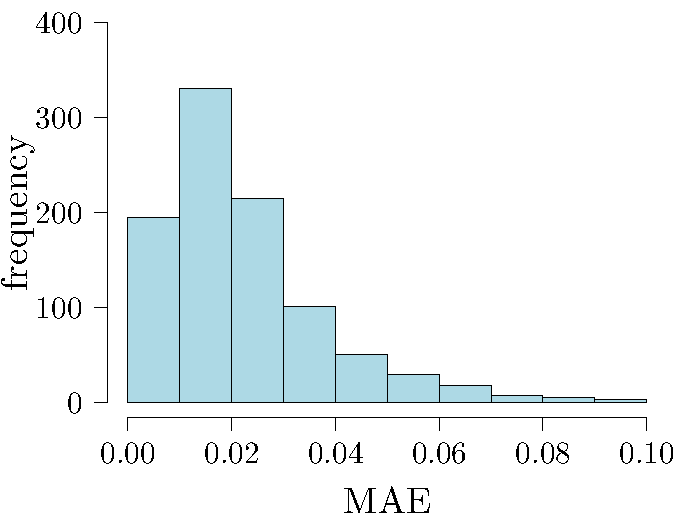
\includegraphics[width=3.5 in]{MAE_histgram_random_controllers.pdf}
		}\\
		\subfloat[(b) \label{fig:AE_box_random_controllers}]{%
			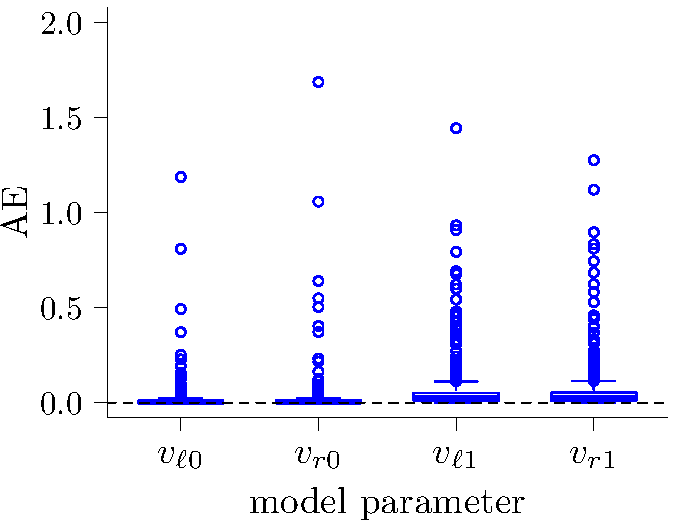
\includegraphics[width=3.5 in]{AE_box_random_controllers.pdf}
		}
		\caption{This plot shows (a) a histogram of the MAE (defined in Equation~\eqref{eq:MAE}) of the evolved models and (b) the AEs (defined in Equation~\eqref{eq:AE}) of each model parameter in the $1000^\textrm{th}$ generation over $1000$ random behaviors. For each behavior, we performed one coevolution run. In (a), $43$ points that have MAE larger than $0.1$ are not shown.}
		\label{fig:model_parameters_random_controllers}
\end{figure}

\subsection{Evolving Other Behaviors}\label{sec:evolving_other_behaviors_swarm_simulation}
The aggregation controller that agents used in our case study was originally synthesized by searching over the space $\left[-1,1\right]^4$, using a metric to assess the swarm's global performance~\cite{Gauci2014_ijrr}. Other points in this space lead to different global behaviors that can be `meaningful' to a human observer (e.g. circle formation~\cite{Melvin_DARS2014}). 
%However, many other controllers may not lead to `meaningful' global behaviors.

We now investigate whether our coevolutionary method can learn arbitrary controllers in this space, irrespective of the global behaviors they lead to. We generated $1000$ controllers randomly in $[-1,1]^4$, with uniform distribution. For each controller we performed one coevolution run, and selected the subjectively best model in the last ($1000^\textrm{th}$) generation. 

Fig.~\subref*{fig:MAE_histgram_random_controllers} shows a histogram of the MAE of the evolved models. The distribution has a single mode close to zero, and decays rapidly for increasing values. Over $89\%$ of the $1000$ cases have an error below $0.05$. This suggests that the accuracy of~\textit{Turing Learning} is not highly sensitive to the particular behavior under investigation (i.e., most behaviors are learned equally well). Fig.~\subref*{fig:AE_box_random_controllers} shows the AEs of each model parameter. The means (standard deviations) of the AEs in each parameter were: $0.01$ ($0.05$), $0.02$ ($0.07$), $0.07$ ($0.6$) and $0.05$ ($0.20$). We performed a statistical test on the AEs between the model parameters corresponding to $I=0$ ($v_{\ell0}$ and $v_{r0}$) and $I=1$ ($v_{\ell1}$ and $v_{r1}$). The AEs of the evolved $v_{\ell0}$ and  $v_{r0}$ were significantly lower than those of the evolved $v_{\ell1}$ and  $v_{r1}$. This was likely due to the reason reported in Section~\ref{sec:analysis_evolved_models_swarm_simulation}; that is, an agent spends more time seeing nothing ($I=0$) than other agents ($I=1$) in each trial.
\begin{figure}[!h]%htbp
	\centering
	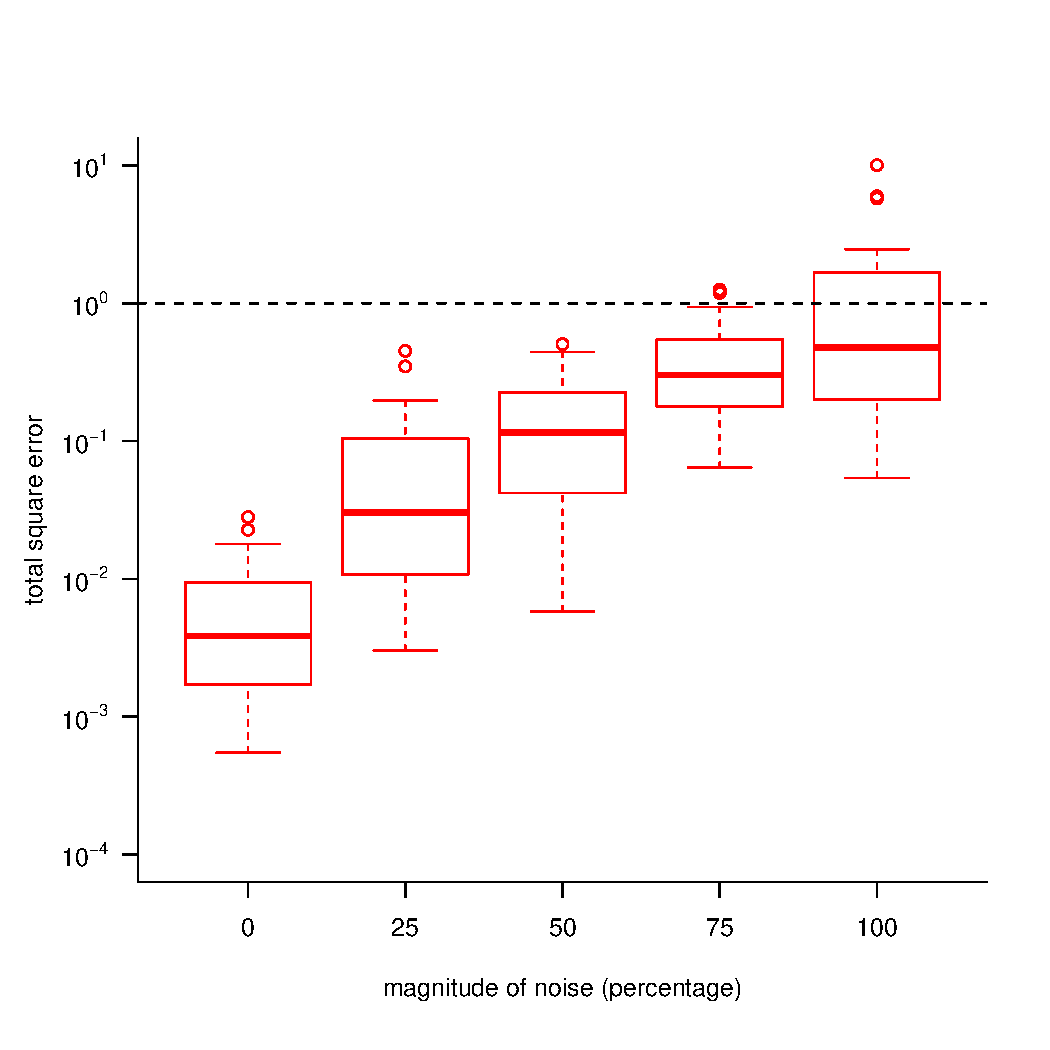
\includegraphics[width=3.5 in]{total_square_error_noise_study.pdf}
	\caption{This plot shows the total square error of the evolved parameters when increasing the percentage of noise on the measurements of the individuals' position and orientation in the aggregation behavior. Each box corresponds to 30 coevolutionary runs. See text for details.
\label{fig:total_square_error_noise_study}}
\end{figure}

\subsection{Noise Study}\label{sec:noise_study_swarm_simulation}

We conducted a study to investigate how the performance of~\textit{Turing Learning} is affected by noise on the measurements of the individuals' position and orientation. As the e-puck robot has a maximum linear speed of $12.8\,\textrm{cm/s}$, the maximum distance that it can travel in one control cycle ($0.1\,\textrm{s}$) is $1.28\,\textrm{cm}$. For this reason, we define a disturbance of $1.28\,\textrm{cm}$ to an individual's position as a measurement error of $100\%$. Similarly, we define a $100\%$ measurement error on the individual's orientation as the maximum change in orientation that an e-puck can undergo in one control cycle. This corresponds to $0.5\,\textrm{rad}$.

We conducted $5$ sets of $30$ coevolutions for the noise values $M=\{0, 25, 50, 75, 100\}\%$. In a coevolution with a noise value $M$, every measurement of an individual's position is perturbed in a random direction and by a random distance chosen uniformly in $\left[0, 1.28\frac{M}{100}\right] \,\textrm{cm}$. Similarly, every orientation measurement is perturbed by a random angle chosen uniformly in $\left[-0.5\frac{M}{100}, 0.5\frac{M}{100}\right]$.

Figure~\ref{fig:total_square_error_noise_study} shows the total square error of the evolved parameters in the final generations of the coevolutions. This plot reveals that the system still performs relatively well when a considerable amount of noise affects the individuals' motion tracking system.

\section{Summary}\label{sec:summary_simulation_swarm}

This chapter has presented the simulation results of using the~\textit{Turing Learning} method to autonomously learn swarm behaviors through observation. To our knowledge, \textit{Turing Learning} is the first system identification method that does not rely on any predefined metric to quantitatively gauge the difference between agents and learned models. This eliminates the need to choose a suitable metric and the bias that such metric may have on the obtained solutions. 

Through competitive coevolution of models and classifiers, the system successfully learned two swarm behaviors (self-organized aggregation and object clustering). Both the model parameters, which were automatically inferred, and emergent global behaviors closely matched those of the original swarm system. We also constructed a robust classifier system that, given an individual's motion data, can tell whether the individual is an original agent or not. Such classifier system could be effective in detecting abnormal behavior, for example, when faults occur in some members of the swarm. Note that~\textit{Turing Learning} produces these classifiers automatically without the need to define a priori what constitutes abnormal behavior. 
%The performance of the classifier system was better than that of any single classifier, as the classifiers were found to collaborate in the coevolution. 

A scalability study showed that the interactions in a swarm can be characterized by the effects on a subset of agents. In other words, when learning swarm behaviors especially with large number of agents, instead of considering the motion of all the agents in the group, we could focus on a subset of agents. This becomes critical when the available data about agents in the swarm is limited. Our approach was proven to work even if using only the motion data of a single agent and replica, as the data from this agent implicitly contained enough information about the interactions in the swarm.   

In this thesis, the model was explicitly represented by a set of parameters. The evolved parameters could thus be compared against the ground truth, enabling us to objectively gauge the quality of evolved models in two case studies as well as for $1000$ randomly sampled behaviors. In principle, we could also evolve the structure of the agent's control system. The results of learning the agent's angle of view showed that our method may even learn the morphology of the swarming agents.
%However, this should not be considered as an inherent limitation of our method. , using an implicit representation (e.g. neural network)
%In the two case studies investigated, the behaviors of the agents in the group were almost not affected by inserting the replica in each trial. 

In collective behavior, abnormal agent(s) may have a great impact on the swarm~\cite{Bjerknes2013}. For the same reason, the insertion of a replica that exhibits different behavior or is not recognized as con-specific may disrupt the global behavior and hence the models obtained may be biased. An appropriate strategy would be to isolate the influence of the replica. In particular, to evaluate a model one could perform two trials, one with only replicas each executing the model and the other with only agents. The data of the replicas and agents from each trial could then be fed into the classifiers for making judgments. Some preliminary results suggest that there is no significant difference between either approach for the case studies considered in this paper.



\chapter{A Real-World Validation of Turing Learning}\label{ch:swarm_physical_implementation}
In this chapter, we present a real-world validation of our coevolutionary approach using a swarm of physical e-puck robots. Unlike the simulation, the evolution in physical systems would become much harder as there would be numerous noises. Moreover, since the simulation could not model the exact dynamics (such as collision) in reality, in the physical coevolutionary experiments we still need to deal with uncertainties which will be discussed later in the implementation. Evolution on physical systems breaks the gap between simulation and reality and could bring us new insight on how to implement evolution in real world. Here we detail the implementation of a complete system for learning the aggregation behavior in Chapter~\ref{ch:swarm_simulation} with minimal human intervention, and discuss the results obtained. 

This chapter is organized as follows. Sec.~\ref{sec:experimental_setup} introduces the physical setup, including robot arena, robot platform and sensor implementation. Sec.~\ref{motion_capture_and_video_processing} details the motion capture and video processing. Sec.~\ref{pc_and_robot_programs} presents the programs executed by the robots and the machine. Sec.~\ref{sec:experimental_protocol} describes the experimental setup and protocol. Sec.~\ref{sec:experimental_results} discusses the results obtained. Sec.~\ref{sec:analysis_algorithm} analyzes the sensitivity of the coevolutionary approach for individual failures during the experiments. Sec.~\ref{sec:summary_swarm_physical} summaries the results obtained and discusses the findings.

\section{Physical Platform}\label{sec:experimental_setup_swarm_physical}
The physical platform, shown in Fig.~\ref{fig:physical_system_setup}, consists of an arena with robots (representing agents or replicas), a personal computer (PC) and an overhead camera. The PC runs the coevolutionary algorithm\footnote{The evolution of the model population could in principle be conducted on the on-board micro-controller of the e-puck, but running it on the PC reduces experimental time~\cite{Floreano1996}.}. It communicates with the replicas, issuing them with models to be executed, but does not exert any control over the other agents. The overhead camera supplies the PC with a video stream of the swarm. The PC performs video processing to obtain motion data about individual robots.
We will now detail these various components.

\begin{figure}[!t]
    \centering
    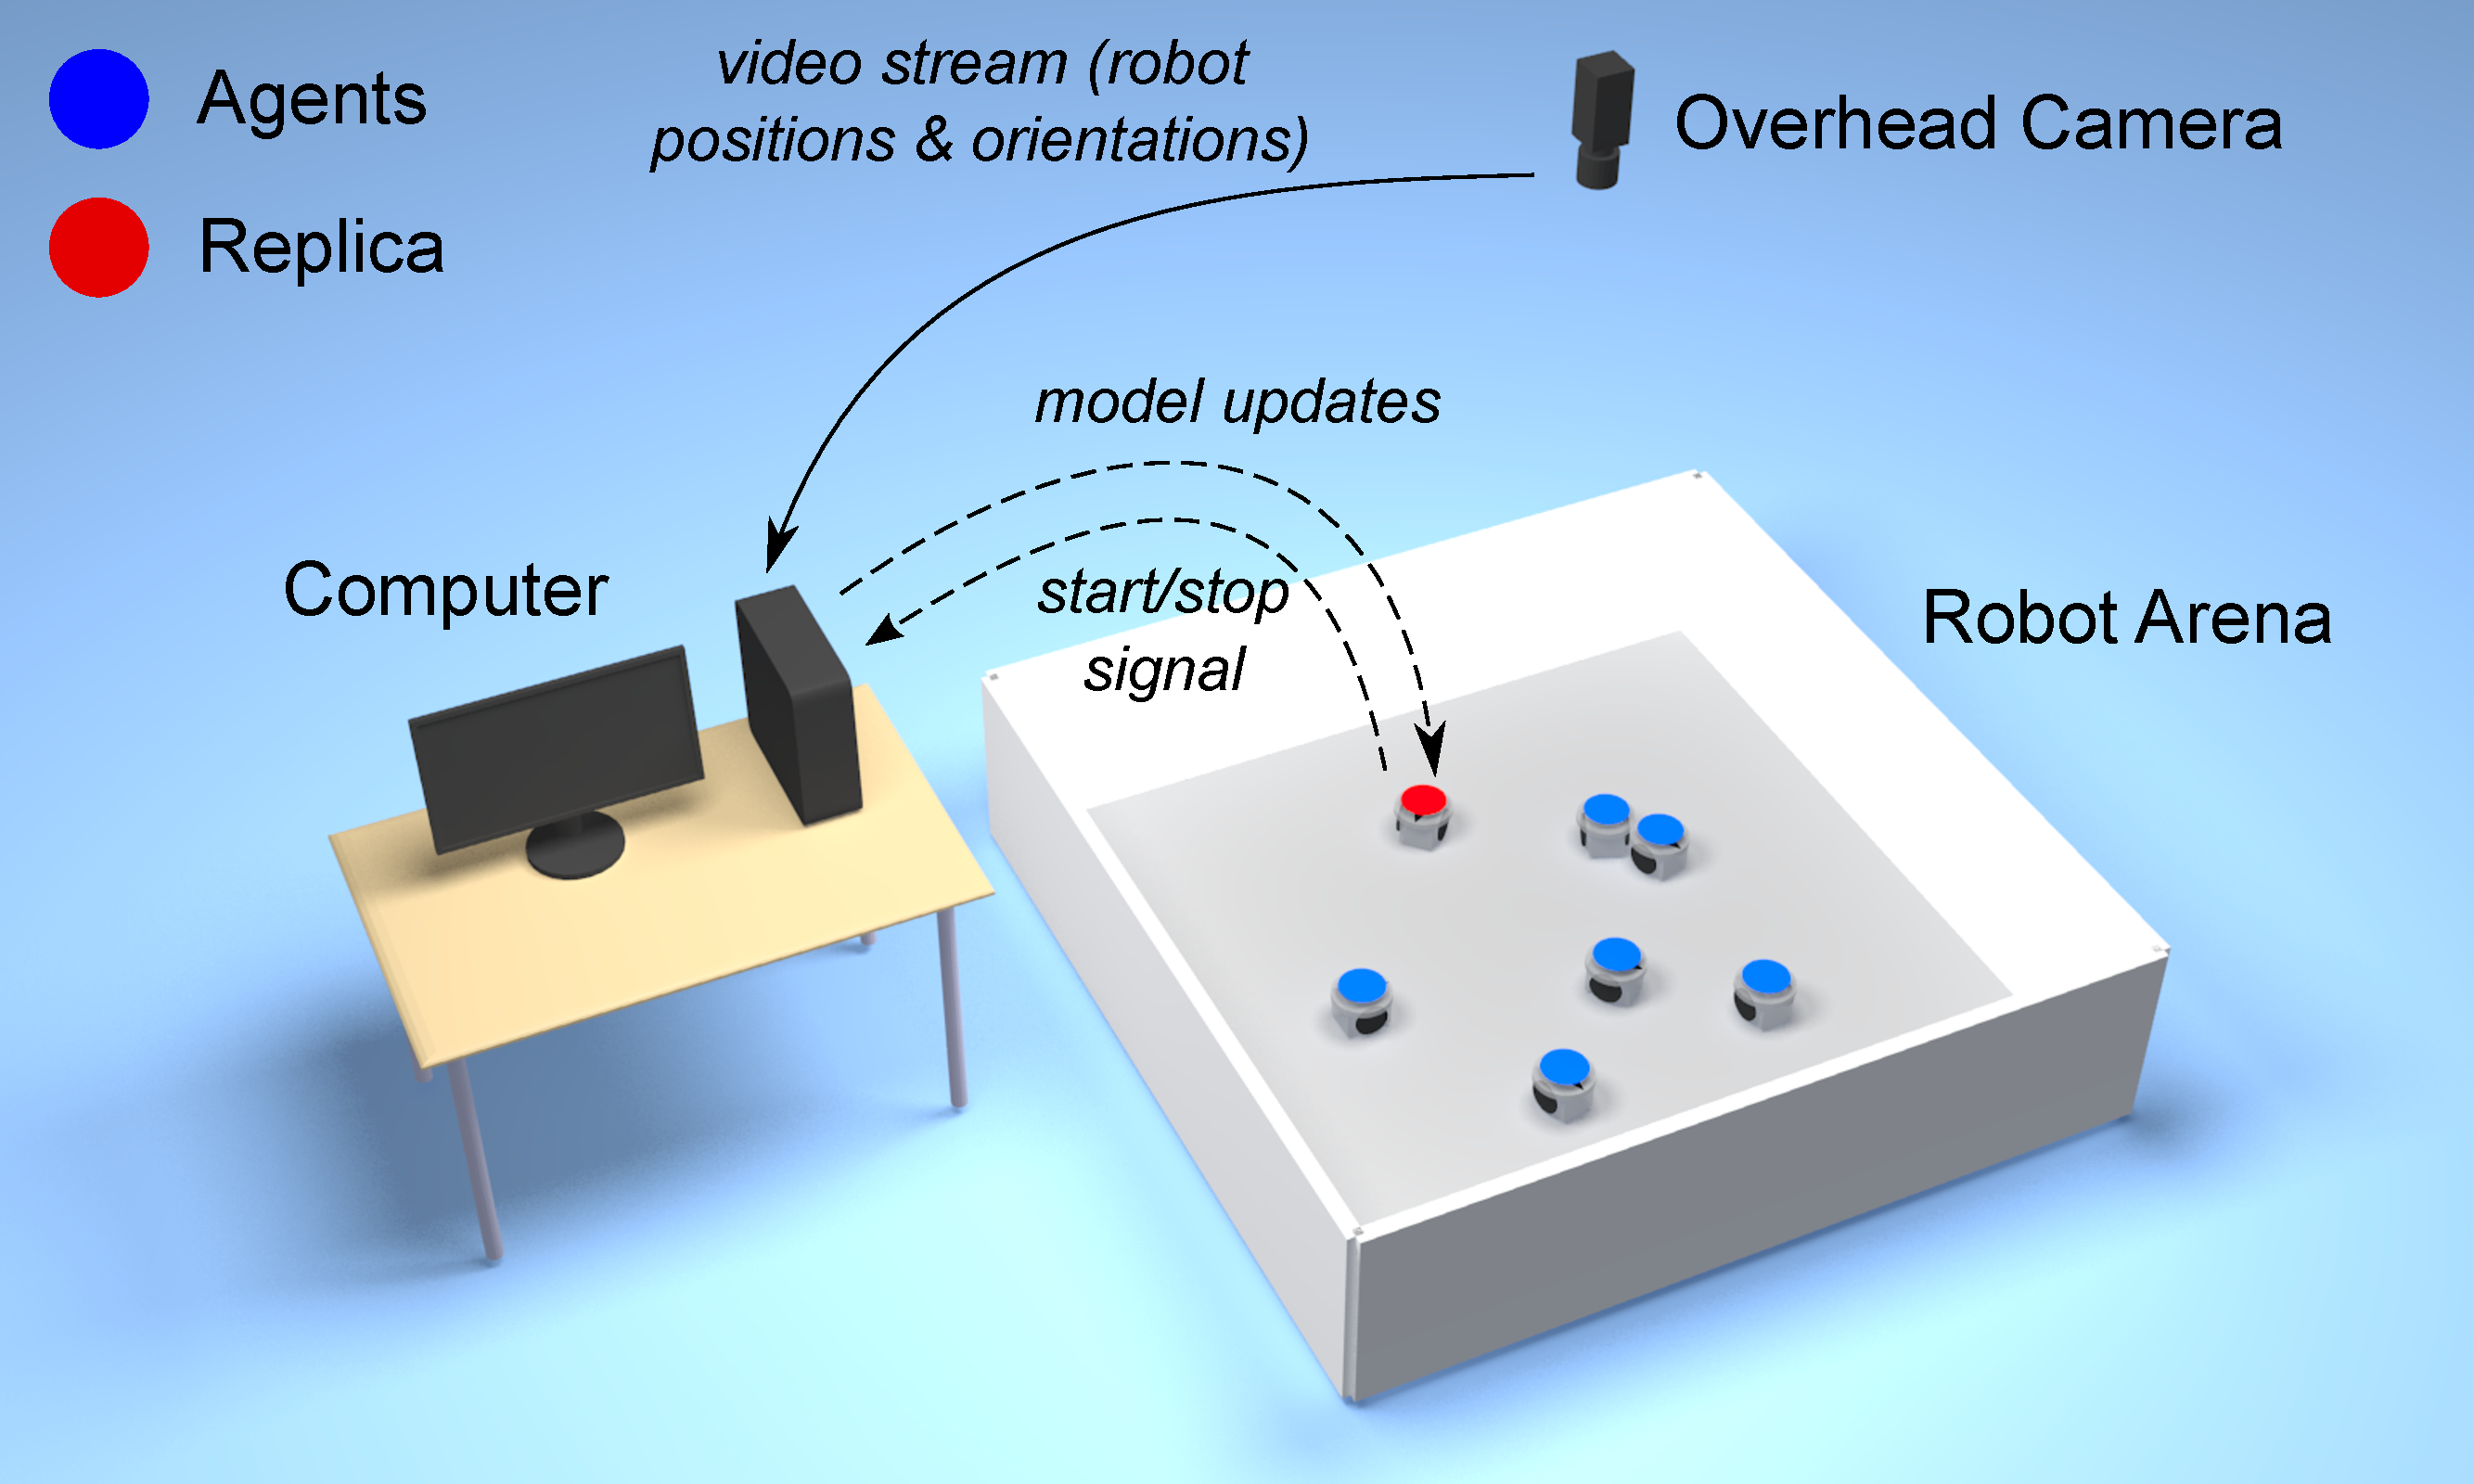
\includegraphics[width=3.5in]{physical_system_setup.pdf}
    \caption{The physical setup. }
    \label{fig:physical_system_setup}
\end{figure} 

\begin{figure}[!t]
	\centering
	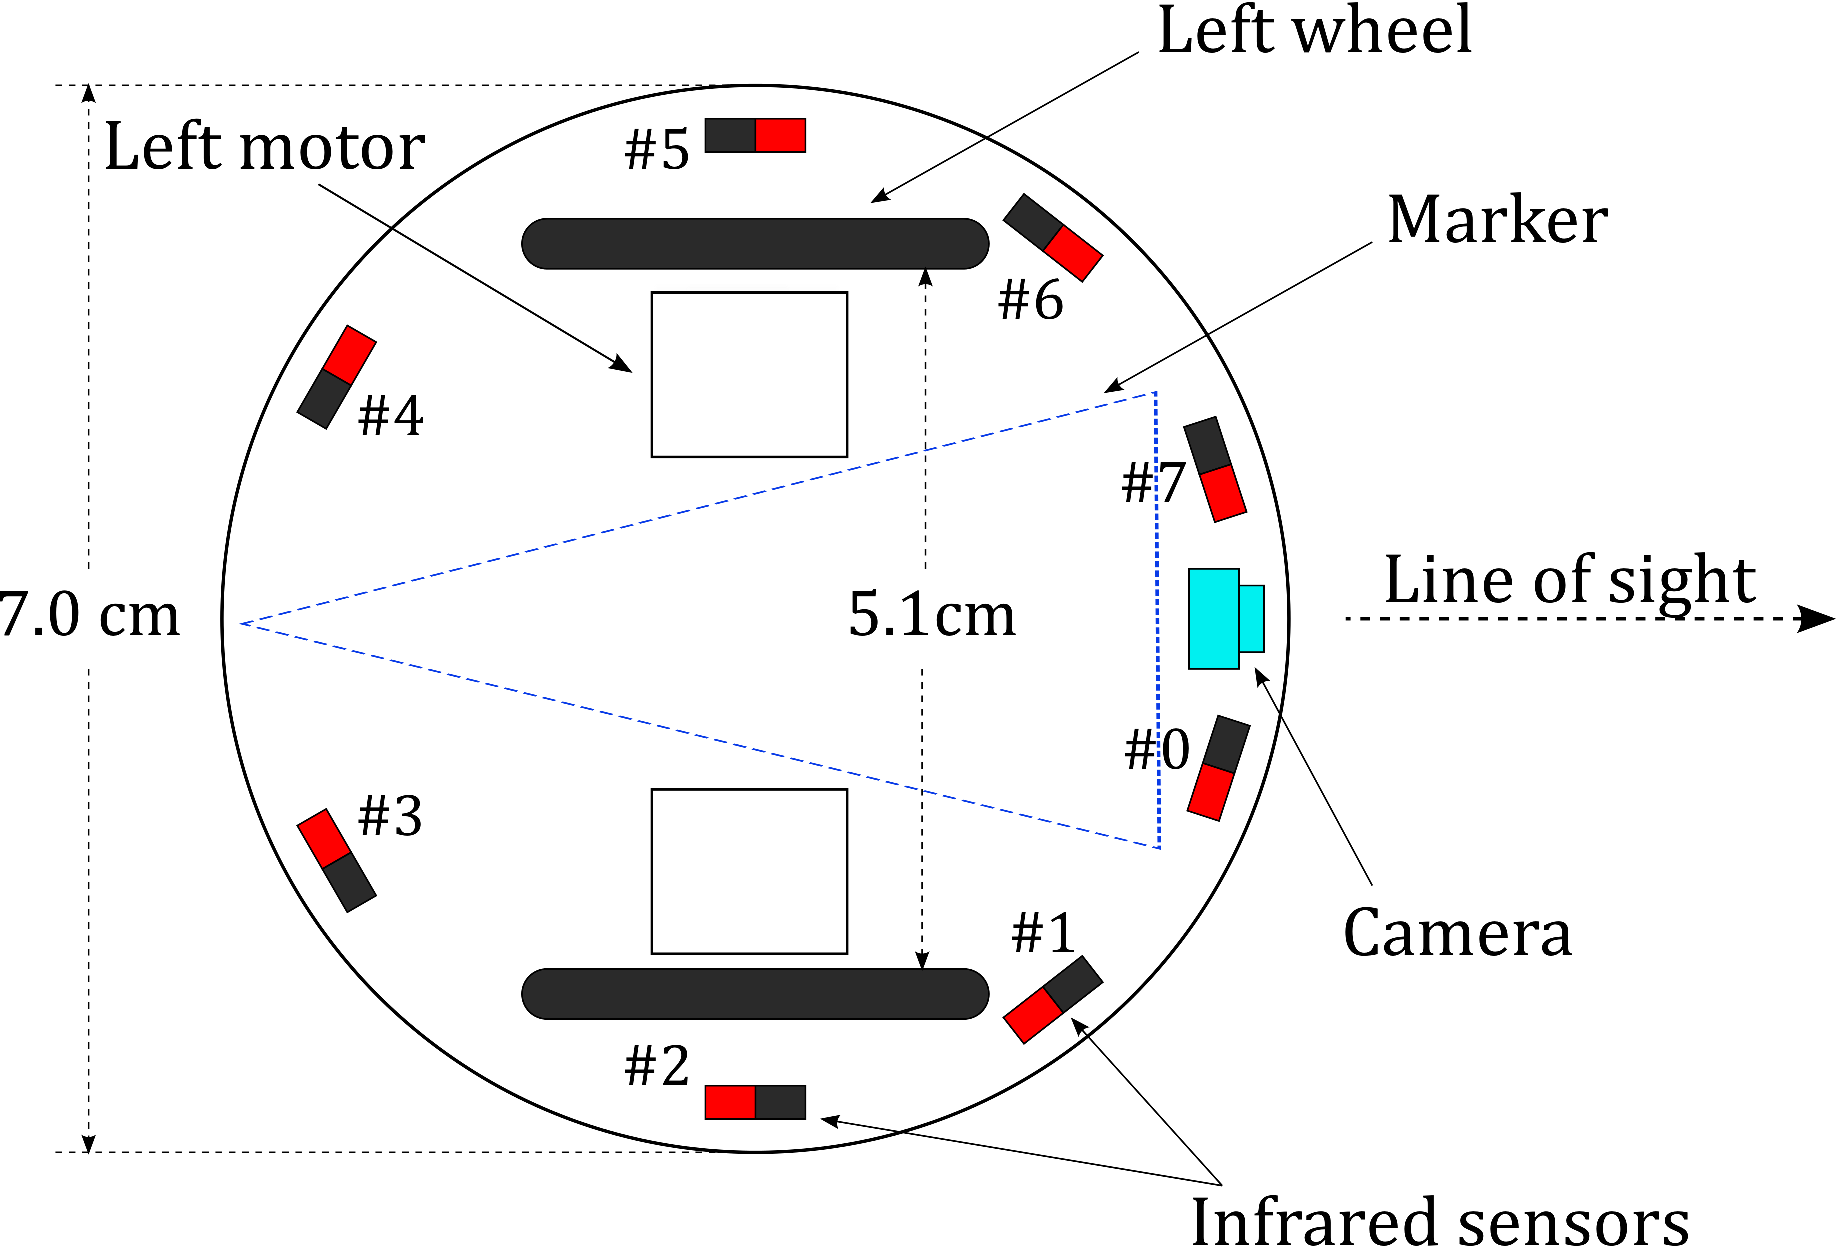
\includegraphics[width=3.5in]{drawing_epuck_schematic.pdf}
	\caption{Schematic top-view of an e-puck, indicating the locations of its motors, wheels, camera and infrared sensors. Note that the marker is pointing towards the robot's \emph{back}.}
	\label{fig:e_puck_schematic}
\end{figure}

\subsection{Robot Arena}

The robot arena was rectangular with sides $\unit[200]{cm} \times \unit[225]{cm}$, and bounded by walls $\unit[50]{cm}$ high. The floor had a light gray color, and the walls were painted white. 

\subsection{Robot Platform and Sensor Implementations}\label{sec:robot_platform_sensor_implementation}

\subsubsection{Robot Platform}
In Chapter~\ref{ch:swarm_simulation}, we presented the e-puck's shape and dimensions as a basis for the agents' embodiment in simulation. We now present further details about the e-puck relevant to our physical implementation. 

The e-puck has a directional camera located in its front. The resolution of the camera is up to $640\times480$, corresponding to the horizontal and vertical angle view of $56\degree$ and $48\degree$. The image is sub-sampled to $40\times15$ pixels due to the limited memory size of the on-board micro-controller, which is the Microchip dsPIC30F6014A with 8KB of RAM and 144 KB of flash memory. There are eight infrared proximity sensors around the body of the robot. These are only used for collision/wall avoidance in the physical coevolutions where the environment is bounded. In the e-puck, the light-of-sight sensor is implemented using the middle column of the pixels from the camera~\citep{Gauci2014_ijrr}. If any pixel of that column exceeds a certain threshold in its gray scale, the sensor outputs $1$; otherwise, it outputs $0$. A schematic top view of the e-puck, showing the sensors and actuators used, is shown in Fig.~\ref{fig:e_puck_schematic}.

\subsubsection{Sensor Implementations}

We implemented the line-of-sight sensor using the e-puck's directional camera, located at its front. For this purpose, we wrapped the robots in black `skirts' (see Fig.~\ref{fig:e-puck_body}) to make them distinguishable against the light-colored arena.  However, we use the camera in monochrome mode, and sub-sample the image to $40 \times 15$ pixels, due to the e-puck's limited memory (which cannot even store a single full-resolution image). While in principle the sensor could be implemented using one pixel, we used a column of pixels from a sub-sampled image to compensate for misalignment in the camera's vertical orientation. The gray values from these pixels were used to distinguish robots ($I=1$) against the arena ($I=0$). For more details about this sensor realization, see~\cite{Gauci2014_ijrr}.

We also used the e-puck's infrared sensors, for two reasons. Firstly, we observed that using only the line-of-sight sensor for aggregation often leads to robots becoming stuck against the walls of the arena, hindering the coevolutionary process. We therefore used the infrared sensors for wall avoidance, but in such a way as to not affect inter-robot interactions.
Secondly, before each trial, the robots dispersed themselves within the arena (behavior \textit{R1} in Sec.~\ref{pc_and_robot_programs}). In this case, we used the infrared sensors to avoid both robots and walls, making the dispersion process more efficient. In the following, we details the implementation of these two programs (\textit{disperse} program and~\textit{wall avoidance} program). 

1) The implementation of~\textit{disperse} program after a trial:

After finishing a trial, we disperse the robots for a while (which is equivalent to initial configuration for a new trial) in order to automate the coevolutionary learning process. This program consists of two behaviors---obstacle avoidance and disperse. The obstacle avoidance behavior is to prevent the robots colliding with other robots and the walls. In particular, before executing the disperse behavior, each robot detects whether some other objects (robots/walls) exist around it through emitting pulses of infrared light and measuring their reflections. If it detects something, it moves away from the objects through adjusting the linear and angular speed accordingly using a single-layer neural network controller. The obstacle avoidance behavior lasts for 3 seconds. In the disperse behavior, each robot is moving forward with a fixed linear speed while avoiding collisions with other robots and the walls. This behavior lasts for 5 seconds.

2) The implementation of~\textit{wall avoidance} program during a trial:

During a trial, in order to reduce the chances of robots getting stuck against the walls (note that the aggregation behavior was designed in an unbounded environment), we implemented the wall avoidance behavior, but in such a way as to not affect inter-robot interactions. In particular, when the robot detected the white walls using the infrared sensors or saw another robot ($I=1$) using the camera, it executed the same behavior. For example, for the agent, it would also turn on the spot when detecting the walls, which makes it easier to avoid the walls. However, the behavior of the replica depends on the model it is executing. Different from the Disperse program, the program of wall avoidance was only triggered when the value of any of the robot's infrared sensor was above a pre-set high threshold. This ensures that the value of the robot's infrared sensors when other robots (covered with a black 'skirt') were nearby was always below the threshold. Therefore, the wall avoidance program did not affect the aggregation of robots.

\section{Motion Capture and Video Processing}\label{motion_capture_and_video_processing_swarm_physical}

\subsection{Motion Capture}

To facilitate motion data extraction, we fitted robots with markers on their tops, consisting of a colored isosceles triangle on a circular white background. The triangle's color allowed for distinction between robots; we used blue triangles for all agents, and orange and purple triangles for the two replicas. The triangle's shape eased extraction of robots' orientations. Note that the orientation of the triangle is pointing to the backward of the e-puck robot so that it can be easily attached.

The robots' motion was captured using a GigE color camera (Basler Technologies), mounted around $\unit[300]{cm}$ above the ground. The camera's frame rate was set to $\unit[10]{fps}$. The video stream was fed to the PC, which performed video processing to extract motion data about individual robots (position and orientation). The size of the arena in the image is 
$\unit[700]{pixels} \times \unit[800]{pixels}$. An image of the arena is shown in Fig.~\ref{fig:robot_arena}.
%
\begin{figure}[!t]
    \centering
    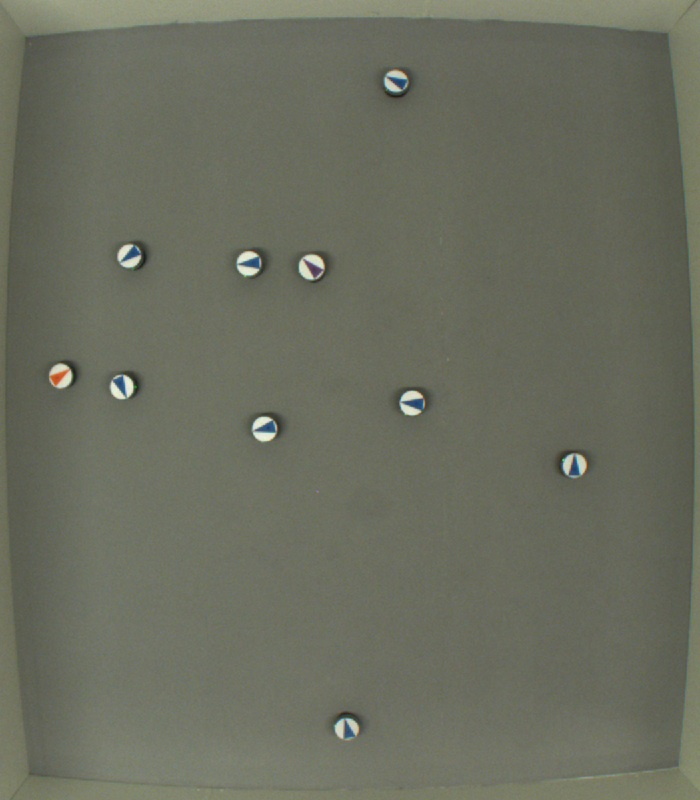
\includegraphics[width=3.0in]{robot_arena.jpg}
    \caption{An image of the robot arena captured by the overhead camera. The robots inside the arena are covered with a colored triangle for facilitating the motion tracking.}
    \label{fig:robot_arena}
\end{figure} 
%
\subsection{Video Processing}

The video processing software was written using OpenCV---an open-source computer vision library~\cite{Gary2008}. The details of the video processing algorithm will be described as follows. 

The image captured using the overhead camera was encoded using RGB. We changed the encoding into HSV in order to make the tracking algorithm less sensitive to lighting variation. This was realized using a built-in function inside the OpenCV library. After that, the image was converted into grayscale and thresholded. As the background of the arena was light-colored, there was no need to do background extraction. After that, we got some binary images. A morphological operation (erosion followed by dilation) is applied on the binary images to filter some noise. Blobs in the binary image with a size above certain threshold (36 pixels) are used for robot detection. These selected blobs indicate the robots in the arena. Fig.~\ref{fig:binary_image_individuals} shows the selected blobs in an image. 
%
\begin{figure}[!t]%
	\centering
		\subfloat[(a) Agents\label{fig:binary_agents}]{%
			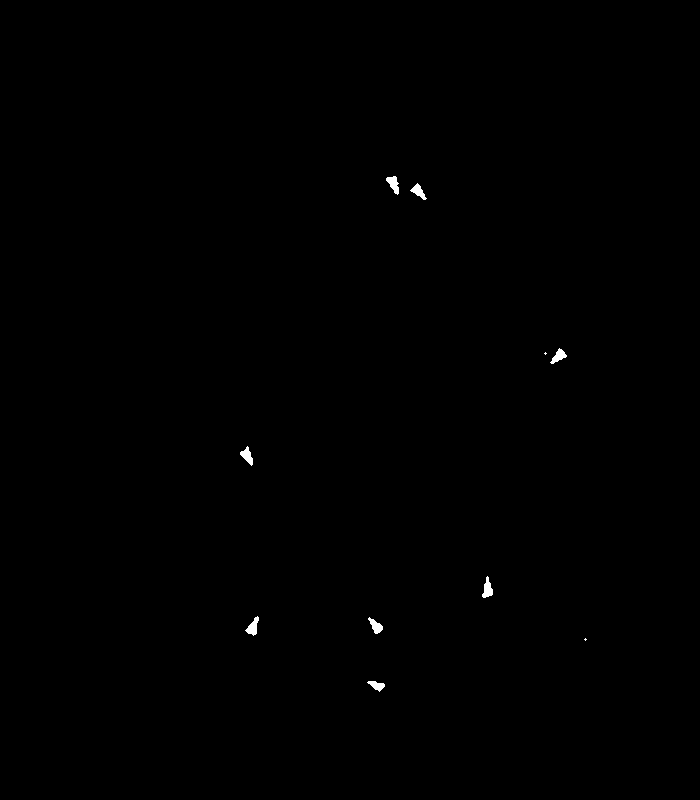
\includegraphics[width=1.65 in]{binary_agents.png} %grid_visualization
		}
		\subfloat[(b) Replica one\label{fig:binary_model_one}]{%
			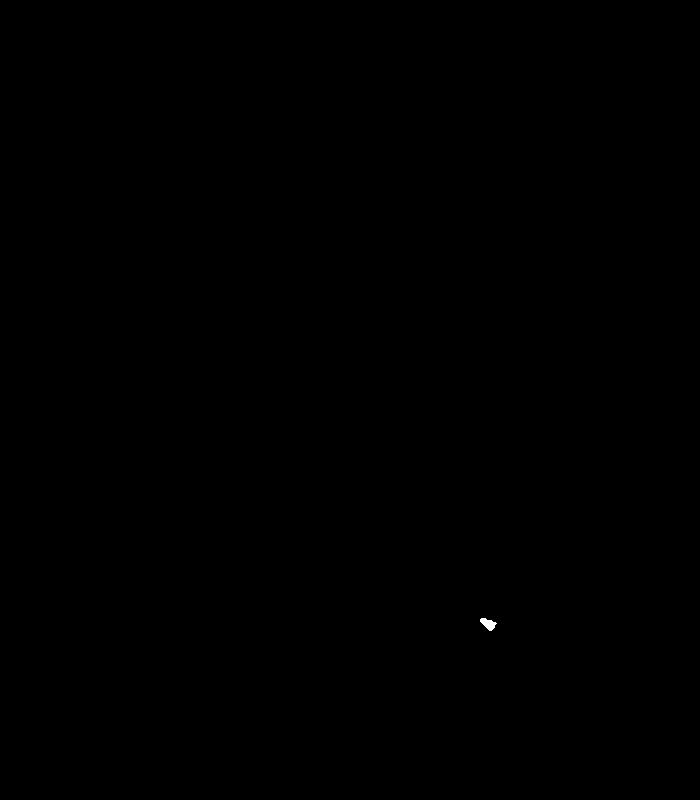
\includegraphics[width=1.65 in]{binary_model_one.png}
		}
		\subfloat[(c) Replica two\label{fig:binary_model_two}]{%
			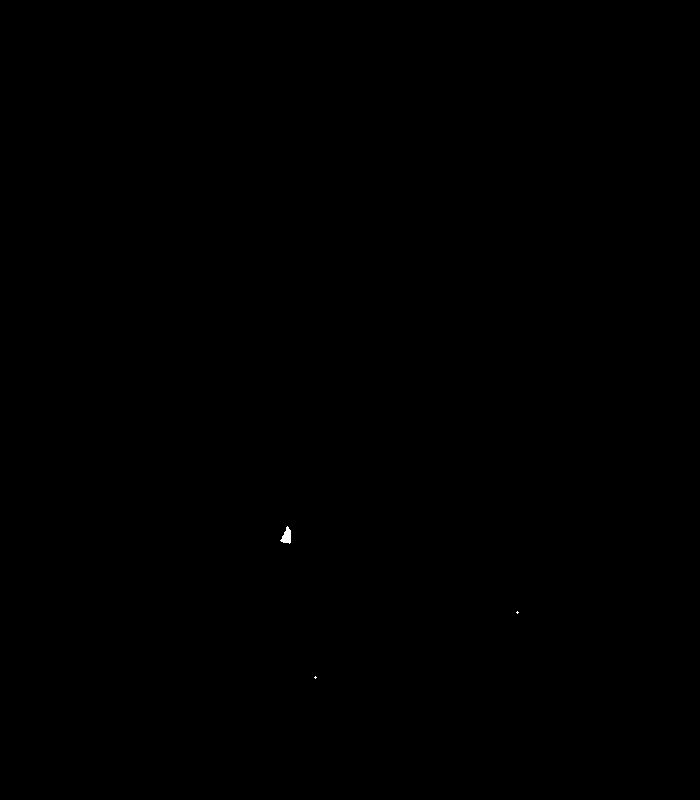
\includegraphics[width=1.65 in]{binary_model_two.png}
		}
		\caption{The images showing the blobs of the robots in the arena. The blobs are selected according to certain compactness and size.}
		\label{fig:binary_image_individuals}
\end{figure}
%

The robots were tracked using the nearest neighbor algorithm. For each blob in the image, we found a minimum triangle that encloses the marker, and got the coordinates of the three vertices of this triangle. The vertex that has the longest distance to the other two vertices indicates the direction of the robot. Therefore the orientation of the robot was estimated using the vector pointing from the midpoint of the other two vertices to this vertex. We use moments~\citep{Hu1962} to calculate the position of the center of the robot. The x and y coordinate of the position is the $1^\mathrm{th}$ order spatial moments around x-axis and y-axis divided by the $0^\mathrm{th}$ order central moments of the blob, respectively. Fig.~\ref{fig:image_processing_flow} shows a diagram of the video processing. 
%
\begin{figure}[!t]
    \centering
    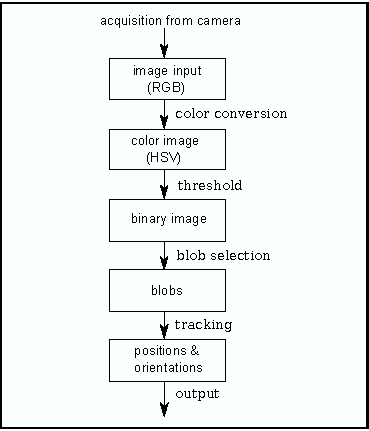
\includegraphics[width=3.5in]{image_processing_flow.pdf}
    \caption{A diagram showing the flow of image processing used in the tracking system.}
    \label{fig:image_processing_flow}
\end{figure} 
%
%
\begin{figure}[!t]
    \centering
    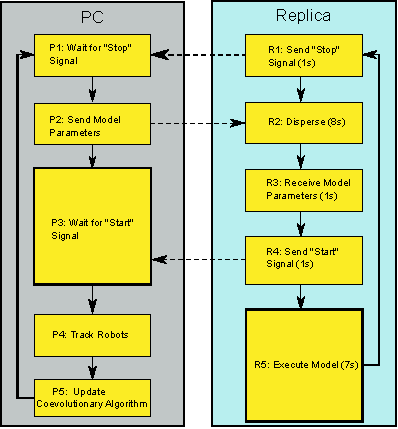
\includegraphics[width=3.5in]{replica_pc_interation.pdf}
    \caption{Schematic of the programs run by the PC and a replica in the physical experiments. Dotted arrows represent communication between the two units. See Sec.~\ref{pc_and_robot_programs} for details.}
    \label{fig:agent_pc_interation}
\end{figure} 
%
\section{PC and Robot Programs}\label{pc_and_robot_programs_swarm_physical}
To automate the coevolutionary process, the PC and robots executed fixed behavioral loops with predefined timings. The PC communicated with the replicas via Bluetooth (we used two replicas to speed up the coevolutionary process, as will be explained in Sec.~\ref{sec:experimental_protocol}) . This served for the PC to issue the replicas with models to be executed, and to synchronize the PC with the swarm. The agents did not perform any communication. At the start of a coevolution run, or after a human intervention (see Sec.~\ref{sec:experimental_protocol}), robots were synchronized using an infrared signal from a remote control.

Fig.~\ref{fig:agent_pc_interation} shows a schematic of the programs run by the PC and the replicas. These programs are represented in terms of various states, with dotted arrows indicating communication between the units. The agents executed a similar behavioral loop to the replicas. Next, we detail the states of the programs executed by the PC, replicas, and agents.

\subsection{PC Program}
\begin{itemize}
	\item \textit{P1:} \textit{Wait for ``Stop'' Signal.} The program is halted until ``Stop'' signals are received from the replicas. These signals indicate that a trial has finished.
	
	\item \textit{P2:} \textit{Send Model Parameters.} The PC sends new model parameters to each replica. These go to the replicas' buffers as the replicas are still in state \textit{R2}; they are later read by the replicas in state \textit{R3}.
	
	\item \textit{P3:} \textit{Wait for ``Start'' Signal.} The program is halted until ``Start'' signals are received from the replicas, indicating that a trial is starting.
	
	\item \textit{P4:} \textit{Track Robots.} The PC waits one second and starts tracking the robots' motion using the overhead camera. While the trial is run for seven seconds (see \textit{R5}), tracking is only performed during the middle five, to discard potentially noisy data from the beginning and end.
	
	\item \textit{P5:} \textit{Update Coevolutionary Algorithm.} The PC performs a fitness update step in the coevolutionary algorithm. The motion data from the trial observed in \textit{P4} is used to update the fitness of the corresponding two models and all the classifiers (according to the procedure described in Chapter~\ref{ch:swarm_simulation}. If all models in the current generation have been evaluated, the PC also generates new model and classifier populations. The PC then goes back to \textit{P1}.
\end{itemize}

\subsection{Replica Program}
\begin{itemize}

\item \textit{R1}: \textit{Send ``Stop'' Signal.} After a trial stops, the replica informs the PC by sending a ``Stop'' signal. 
The PC sends a new model to the replica's buffer.
The replica waits one second before moving to \textit{R2}, so that all robots remain synchronized (agents are programmed to restart one second after a trial stops). Waiting one second in other states serves the same purpose.

\item\textit{R2}: \textit{Disperse.} The replica disperses in the environment, while avoiding collisions with other robots and the walls. This behavior lasts eight seconds.

\item\textit{R3}: \textit{Receive Model Parameters.} The replica reads new model parameters from its buffer (sent earlier by the PC). It waits one second before moving to \textit{R4}.

\item\textit{R4}: \textit{Send ``Start'' Signal.} The replica sends a start signal to the PC to inform it that a trial is about to start. The PC prepares to start tracking the robots' motion. The replica waits one second before moving to \textit{R5}.

\item\textit{R5}: \textit{Execute Model.} The replica moves within the swarm according to its model. This behavior lasts seven seconds. The replica then moves back to \textit{R1}.
\end{itemize}
%A video showing a cycle of the sequential behaviors for the agents and replicas as well as the implementation details of \textit{R2} can be found in the online supplementary material~\cite{online_supplementary_material_tevc2014}.

\subsection{Agent Program}
\begin{itemize}
\item The agents follow the same behavioral loops as the replicas. However, in the states analogous to \textit{R1}, \textit{R3}, and \textit{R4}, they simply wait one second rather than communicate with the PC. In the state corresponding to \textit{R2}, they also execute the \textit{Disperse} behavior. In the state corresponding to \textit{R5}, they execute the real aggregation controller, rather than a model.
\end{itemize}

\section{Experimental Setup and Protocol}\label{sec:experimental_protocol_swarm_physical}
In the coevolutionary algorithm, we used population sizes of $20$ for models, and $100$ for classifiers (as opposed to $100$ models in the simulated coevolutions of Chapter~\ref{ch:swarm_simulation}; this was done to reduce experimental time). We used $10$ robots in the arena: $8$ representing agents executing the real aggregation controller (Eq.~\eqref{eq:aggregation_optimal_controller}), and $2$ representing replicas that executed models. This meant that in each trial, $2$ models from the population could be evaluated simultaneously; consequently, each generation consisted of $20/2=10$ trials. 
%Note from the previous section that each trial lasted $\unit[18]{s}$; each generation therefore lasted $10\times 18 = \unit[180]{s}$. We chose to run coevolutions for $100$ generations, for a total time of around $5$ hours per run (excepting human interventions).

The coevolutionary algorithm was implemented without any modification to the code used in simulation (except for model population size and observation time in each trial). We still let the model parameters evolve unboundedly (i.e., in $\mathbb{R}^4$). However, as the speed of the physical robots is naturally bounded, we applied the hyperbolic tangent function ($\tanh{x}$) on each model parameter, before sending a model to a replica. This bounded the parameters to $\left(-1,1\right)^4$, with $-1$ and $1$ representing the maximum backward and forward wheel speeds, respectively.

During a coevolution run, a human intervention was made in the following cases. Otherwise, the run proceeded autonomously.
\begin{itemize}
\item The robots had been running continuously for $25$ generations. All batteries were replaced.

\item A robot stopped moving, for example because of a lost battery connection or because it became stuck on the floor. Appropriate action was taken for the affected robot.

\item A replica lost its Bluetooth connection with the PC. The connection (with both replicas) was restarted.

\item A robot indicated a low battery status through its LED after running for only a short time. That robot's battery was changed.
\end{itemize}

After an intervention, the ongoing generation was restarted, to limit the impact on the coevolutionary process.

%In each situation, either the batteries or robots were changed. To limit the impact on the evaluation, the current generation was rerun. %, otherwise the robots would stop working for the rest of trials 

%In order to reduce the chances of robots getting stuck on the wall (note that the aggregation behavior was designed in an unbounded environment), the aggregation behavior was modified. When the robot detected the wall using the four proximity sensors in its back (sensors 2, 3, 4, 5 in Fig.~\ref{fig:e_puck_schematic}), it behaved as if $I=1$ (for example,  the agent would turn on the spot). This action was only triggered when the sensory value was above a certain threshold. Since the robots were covered with a black `skirt', the value of the proximity sensors was very low when two robots were near each other, therefore this action did not affect the aggregation behavior. 
%
\begin{figure}[!t]
    \centering
    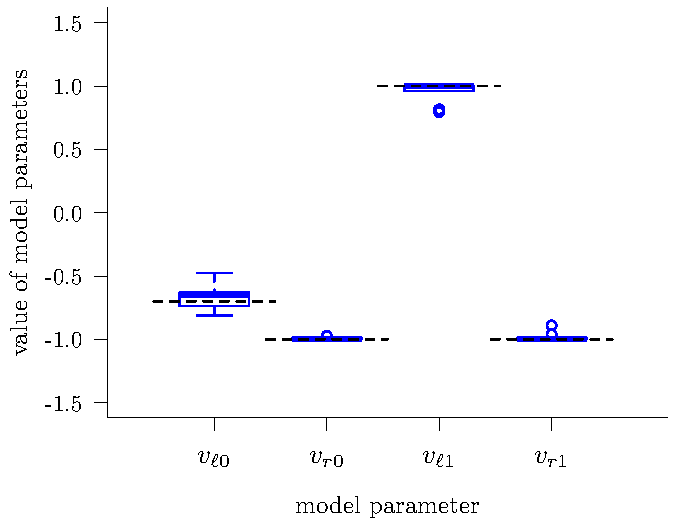
\includegraphics[width=3.5in]{best_model_parameters_physical.pdf}
    \caption{Parameters of the evolved models in the $100^{\textrm{th}}$ generation of $10$ physical coevolution runs. Dotted black lines indicate true values.}
    \label{fig:best_model_parameters_physical}
\end{figure}
%
\section{Results}\label{sec:experimental_results_swarm_physical}
We conducted $10$ coevolution runs using the physical system. Each run lasted $100$ generations, corresponding to around $5$ hours (excluding human intervention time).
%
%Note from the previous section that each trial lasted $\unit[18]{s}$; each generation therefore lasted $10\times 18 = \unit[180]{s}$. We chose to run coevolutions for $100$ generations, for a total time of around $5$ hours per run (excepting human interventions).
\begin{figure}[!t]%
	\centering
		\subfloat[(a) Simulated Coevolutions\label{fig:model_parameters_convergence_compare_simulation}]{%
			\includegraphics[width=3.5 in]{model_parameters_convergence_compare_simulation.pdf} %grid_visualization
		}\\
		\subfloat[(b) Physical Coevolutions\label{fig:model_parameters_convergence_compare_physical}]{%
			\includegraphics[width=3.5 in]{model_parameters_convergence_compare_physical.pdf}
		}
		\caption{Evolutionary progress of each model parameter in $10$ (a) simulated and (b) physical coevolution runs. Curves represent median values across $10$ runs. Dotted black lines indicate true values.}
		\label{fig:model_parameters_convergence_compare}
\end{figure}
%
\subsection{Post Evaluation}
 To select the `best' model from each coevolution run, we post-evaluated all evolved models in the final generation $5$ times using all classifiers in that generation. The parameters of these models are shown in Fig.~\ref{fig:best_model_parameters_physical}. The means (standard deviations) of the AEs in each parameter were: $0.08$ ($0.06$), $0.01$ ($0.01$), $0.05$ ($0.08$), and $0.02$ ($0.04$).

To investigate the effects of real-world conditions on the coevolutionary method, we performed $10$ simulated coevolution runs with the same setup as in the physical runs.
Fig.~\ref{fig:model_parameters_convergence_compare} shows the evolutionary dynamics of the evolved model parameters in the simulated and physical coevolution runs.
Figures~\subref*{fig:model_parameters_convergence_compare_simulation}  and~\subref*{fig:model_parameters_convergence_compare_physical} show that the dynamics show good correspondence overall. However, the convergence in the physical coevolutions is somewhat less smooth than that in the simulated ones (e.g., the spikes in $v_{\ell0}$ and $v_{l1}$). One reason for this may be the limitations in motion data capture and extraction. In particular, given the relatively small diameter of the e-puck in our arena, inferring its orientation is particularly challenging.

We will now investigate the classifiers' performance. In each generation 
of every coevolution run (simulated and physical), we computed the MAE of each model. We compared the error of the model with the highest subjective fitness with the average and lowest errors. The results are shown in Fig.~\ref{fig:MAE_compare_simulation_physical}.
In both the simulated and physical cases, the subjectively best model (green) has an error in between the average (red) and the lowest (blue) in the majority of generations. Also in both cases the gap between the error of the subjectively best model and the average error becomes wider as the coevolution proceeds, which means the classifiers are only misguided by increasingly good models. This gap, in turn, forces the model population to evolve, as indicated by the downwards trend of the lowest error.
%
% Fig.~\subref*{fig:model_parameters_convergence_compare_physical}, the error of the models with the highest objective fitness is becoming smaller until about $60^\textrm{th}$ generation, and then it increases slightly. We suspect that this is due to the fact that when the replica behaves more like the agents (that is, the model parameters converge to their real value), it is more likely to collide with them (i.e., to aggregate). the chance of its collision with other agents is higher than those replicas that executes `worse' models.
%
\begin{figure}[!t]%
	\centering
		\subfloat[(a) Simulated Coevolutions\label{fig:MAE_simulation}]{%
			\includegraphics[width=3.5 in]{MAE_simulation.pdf} %grid_visualization
		}\\
		\subfloat[(b) Physical Coevolutions\label{fig:MAE_physical}]{%
			\includegraphics[width=3.5 in]{MAE_physical.pdf}
		}
		\caption{Evolutionary progress of models in $10$ (a) simulated and (b) physical coevolution runs. Curves represent median values across $10$ runs. The red curve represents the average error of all models in a generation. The green and blue curves show, respectively, the errors of the models with the highest subjective and the highest objective fitness in a generation.}
		\label{fig:MAE_compare_simulation_physical}
\end{figure}
%
\begin{figure}[!t]
    \centering
    \includegraphics[width=3.5in]{all_generation_judgment_accuracy_physical.pdf}
    \caption{Average performance of the classifier system selected using the recording data during the trials over $10$ coevolution runs. The error bar shows standard deviation.}
    \label{fig:all_generation_judgment_accuracy_physical}
\end{figure}

In order to further investigate the performance of the classifier system (as discussed in details in Chapter~\ref{ch:swarm_simulation}), we evaluated the evolved classifiers in every $10$ generation using $100$ models\footnote{Note that since it takes too long to perform a grid evaluation as we did in simulation, here we only evaluated the performance of the classifiers using a limited number of random-generated models.}. The parameters of each model were randomly-generated in $[-1,1]^4$. For the details of the selection process of the classifier system, refer to Chapter~\ref{ch:swarm_simulation}. Fig.~\ref{fig:all_generation_judgment_accuracy_physical} shows the performance of the best classifier and the classifier system over generations. Similar to the results obtained in simulation, the classifier system evolved in the physical coevolution runs still has a high performance over the testing individuals (including agents and models). However, in contrast to simulation, the performance of the best classifier did not drop with the increasing generations. This may be due to the reason that it took longer for the models to converge in the physical coevolutionary experiments and the best classifier selected according to the available recording data was not over-specialized as in the simulation. 

\subsection{Model Validation}
As we argued before (Sec.~\ref{sec:analysis_evolved_models}), in swarm systems, good agreement between local behaviors (e.g., controller parameters) is not a guarantee of similar global behaviors. For this reason, we performed $20$ trials using $40$ e-pucks, lasting $10$ minutes each: $10$ with the real controller (Eq.~\eqref{eq:aggregation_optimal_controller}), and $10$ with a controller obtained from the physical coevolution runs. This latter controller was constructed by taking the median values of the parameters over the $10$ runs, which are:
$$
\mathbf{p}=\left(-0.65, -0.99, 0.99, -0.99\right).
$$
The set of initial configurations of the robots was common to both controllers. As it was not necessary to extract the orientation of the robots, a red circular marker was attached to each robot so that its position can be extracted with good accuracy in the offline analysis.
%
\begin{figure}[!t]%
	\centering
		\subfloat[(a) Largest Cluster Dynamics \label{fig:aggregation_dynamics_proportion}]{
			\includegraphics[width=3.5 in]{aggregation_dynamics_proportion.pdf}
		}\\
		\subfloat[(b) Dispersion Dynamics \label{fig:aggregation_dynamics_compactness}]{
			\includegraphics[width=3.5 in]{aggregation_dynamics_compactness.pdf}
		}
		\caption{Average aggregation dynamics in $10$ physical trials with $40$ e-puck robots executing the real controller (red) and the evolved controller (blue). In (a), the vertical axis shows the proportion of robots in the largest cluster; in (b), it shows the robots' dispersion (see Sec.~\ref{sec:analysis_evolved_models}). Dotted lines in (a) and (b), respectively, represent the maximum proportion and minimum dispersion that $40$ robots can achieve.}
		\label{fig:aggregation_dynamics_physical}
\end{figure}
%
Fig.~\subref*{fig:aggregation_dynamics_proportion} shows the proportion of robots in the largest cluster\footnote{A cluster of robots is defined as a maximal connected subgraph of the graph defined by the robots' positions, where two robots are considered to be adjacent if another robot cannot fit between them~\cite{Gauci2014_ijrr}.} over time with the real and evolved controllers. Fig.~\subref*{fig:aggregation_dynamics_compactness} shows the dispersion (as defined in Sec.~\ref{sec:analysis_evolved_models}) of the robots over time with the two controllers. The aggregation dynamics of the real and evolved behaviors show good correspondence. Fig.~\ref{fig:aggregation_snapshoot_physical_validation} shows a sequence of snapshots from a trial with $40$ e-pucks executing the evolved controller.

\begin{figure}[!t]
\centering
\includegraphics[width=3.5in]{aggregation_model_validation_physical.pdf}
\caption{Time taken for different numbers of robots to aggregate into a single cluster. Each box corresponds to $30$ simulation trials with the real controller (red), and the controller obtained from the physical coevolution runs (blue).}
\label{fig:aggregation_model_validation_physical}

\end{figure}

\captionsetup[subfigure]{labelformat=empty}  
\begin{figure*}[!t]
	\centering
	\subfloat[initial configuration]{
		\includegraphics[width = 1.7 in]{physical_snapshot_0s.jpg}
	}
	\subfloat[after $20$ $\unit{s}$]{
		\includegraphics[width = 1.7 in]{physical_snapshot_20s.jpg}
	}\\
	\subfloat[after $40$ $\unit{s}$]{
		\includegraphics[width = 1.7 in]{physical_snapshot_40s.jpg}
	}
	\subfloat[after $180$ $\unit{s}$]{
		\includegraphics[width = 1.7 in]{physical_snapshot_180s.jpg}
	}\\
		\subfloat[after $360$ $\unit{s}$]{
		\includegraphics[width = 1.7 in]{physical_snapshot_360s.jpg}
	}
	\subfloat[after $420$ $\unit{s}$]{
		\includegraphics[width = 1.7 in]{physical_snapshot_420s.jpg}
	}\\
	\subfloat[after $480$ $\unit{s}$]{
		\includegraphics[width = 1.7 in]{physical_snapshot_480s.jpg}
	}
	\subfloat[after $600$ $\unit{s}$]{
		\includegraphics[width = 1.7 in]{physical_snapshot_600s.jpg}
	}
	\caption{Snapshots of the aggregation behavior with $40$ e-puck robots using the model that was automatically learned through observation of swarms of physical robots in the coevolution.}
	\label{fig:aggregation_snapshoot_physical_validation}
\end{figure*}

We also performed a scalability study in simulation to compare the real and evolved controllers. We calculated the time taken to form a single cluster with different numbers of robots: $n \in \lbrace10, 20, \dots, 100\rbrace$. For each number of robots, we performed $30$ trials with each controller. The results are shown in Fig.~\ref{fig:aggregation_model_validation_physical}. In all cases, the real controller slightly outperforms the evolved one.
However, with either controller, the robots aggregate in a relatively short time ($<\unit[600]{s}$). There is a statically significant difference in aggregation times with the two controllers for $n= 10, 30, 50, 70, 80, 90$---but this suggests no particular pattern with respect to $n$. We also performed a linear least squares regression on the aggregation times with the two controllers. The fits were: $T = 53.2 + 2.2n$ for the real controller, and $T = 64 + 2.4n$ for the evolved controller ($n>1$). This indicates that the evolved controller does not scale much worse than the real one.

The video accompanying this paper shows the evolutionary process both in simulation and on the physical system. It also shows the emergent, global behaviors of the real controller and the obtained model on the physical system. Additionally, videos of all $10$ physical coevolution runs, and all $20$ post-evaluation trials with $40$ e-pucks, are available in the online supplementary material~\cite{online_supplementary_material_tevc2014}.

\begin{figure}[!t]
    \centering
    \includegraphics[width=3.5in]{algorithm_sensitivity_analysis.pdf}
    \caption{This plot shows the relationship between the old fitness, $f$, and the new fitness, $F$, of the classifiers, when the failure ratio of agents in the swarm, $\frac{m}{N}$, changes. When $m = 0$ or $N \rightarrow \infty$, $F=f$. When $0 < \frac{m}{N} < 1$, $F$ is shifted, but the fitness order is not changed.}
    \label{fig:analysis_algorithm}
\end{figure}

\section{Analysis of Sensitivity for Individual Failure}\label{sec:analysis_algorithm}

In the physical experiments, we have observed that some robots may get stuck or stop working because of the reasons mentioned in Section~\ref{sec:experimental_protocol}. This could also happen in a real swarm system, for example, some individuals may stop moving or display other abnormal behaviors due to various factors such as collision. These abnormal behaviors (which are considered failure here) may not be recognized during the process of experiments. Therefore, we have analyzed whether abnormal behaviors (failure) of some individuals may bias the evolution and hence affect performance of our proposed coevolutionary approach. Assuming the failure is equally likely to be present in the replica and agent in a trial. We have proved that: \textit{\textbf{the metric-free coevolutionary approach is not biased by failure of certain individuals in the swarm.}} The mathematical proof is provided as follows:
 
\begin{proof}
Let $n$ be the total size of the group, consisting of $n-1$ agents and $1$ replica. $m$ represents the number of individuals that fail ($m<n$) in a trial. $p$ and $q$ are the probabilities of a classifier to make the correct judgment for models and agents respectively. Therefore, the expected fitness of the classifier without failure of any individuals in one generation, $f_c$, is equal to $\frac{p+q}{2}$. $f_m$ denotes the fitness of a model in that generation. 

There are two failure cases: 1) failure with the replica; 2) failure without the replica. We assume that if an individual fails during a trial, the classifier makes random judgment, that is, it has equal probability, which is $50\%$, of judging the individual as an agent or a model. If failure exists in a trial, the probability that failure with the replica occurs, $p_1$, is as follows:
\begin{equation}
{p_1} = {\binom{n-1}{m-1}} / {\binom{n}{m}} = \frac{m}{n}.
\end{equation}
The probability that failure without the replica occurs in a trial, $p_2$, is: $1 - p_1 = \frac{n-m}{n}$. The proof is divided into two parts: one for the classifiers and the other is for models.

For the classifier, the new fitness in the first failure case, $f_{c1}$, can be calculated as follows:
\begin{equation}\label{equ:f1:classifier}
{f_{c1}} = p_1 \cdot (\frac{1}{2} + \frac{1}{2} \cdot \frac{m-1}{n-1} + \frac{q \cdot (n-m)}{n-1}) /2.
\end{equation}
In the second failure case, the new fitness of the classifier, $f_{c2}$, is given by:
\begin{equation}\label{equ:f2:classifier}
{f_{c2}} = p_2 \cdot (p + \frac{1}{2} \cdot \frac{m}{n-1} + \frac{q \cdot (n-m-1)}{n-1}) / 2.
\end{equation}
Combining Eqs.~\eqref{equ:f1:classifier} and~\eqref{equ:f2:classifier} and simplifying the resulting expression, the new fitness, $F_c$, of the classifier when $m$ individuals fail in a trial is:
\begin{equation}\label{equ:F:classifier}
{F_c} = f_{c1} + f_{c2} = f_c \cdot (1-\frac{m}{n}) + \frac{m}{2n}.
\end{equation}

In Eq.\eqref{equ:F:classifier}, $F_c$ is monotonic increasing in terms of $f_c$. When $f_c$, is equal to $0.5$, $F_c$ maintains the same value. When $f_c$ is greater than (or smaller than) $0.5$, $F_c$ is decreased (or increased) but still greater (or smaller) than $0.5$. Therefore, the fitness order of all the classifiers after failure of $m$ individuals in a trial is not changed, which means it does not affect the selection of the classifiers in the evolutionary process. 
%http://www.numberempire.com/simplifyexpression.php Fig.~\ref{fig:analysis_algorithm} visualized how the fitness of the classifiers is shifted when failure of agents occurs. %{F_c} = f_{c1} + f_{c2} = \frac{m}{2N}[1 + (p + q) \cdot \frac{N-m}{m}] = f \cdot (1-\frac{m}{N}) + \frac{m}{2N}.

For the model, it has a new fitness of $f_{m1} = \frac{m}{n} \cdot \frac{1}{2}$ and $f_{m2} = \frac{(n-m) \cdot f_m}{n}$ in the first and second failure case, respectively. Therefore, the new fitness of the model, $F_m$, when $m$ individuals fail in a trial is:
\begin{equation}\label{equ:F:model}
{F_m} = f_{m1} + f_{m2} = f_m \cdot (1-\frac{m}{n}) + \frac{m}{2n}.
\end{equation}
Comparing Eqs.~\eqref{equ:F:classifier} and~\eqref{equ:F:model}, we can see that the fitness order of all the models is also unchanged when failure occurs in a trial.
\end{proof}

\section{Summary}\label{sec:summary_swarm_physical}

In this chapter, we presented a physical autonomous coevolutionary system for identifying the aggregation behavior in Chapter~\ref{ch:swarm_simulation} using swarms of e-puck robots. The behavior was learned successfully, and the results obtained in the physical experiments show good correspondence to those obtained in simulation. This showed the robustness of our metric-free coevolutionary method with respect to noise and uncertainties in real world, which provided a first step towards automated reversing engineering of  swarm behaviors with little human intervention~\cite{King2009, Schmidt2009}. 

The model obtained in the physical coevolution runs was validated using $40$ e-puck robots. The global behavior of the obtained model is similar to that of the real controller. The selected classifier system over the coevolution runs still obtained a high performance, which means our classifier system could be potentially applied to detect or monitor the behaviors of the agents in a swarm. 
% The step of validation is necessary in our approach. As the classifiers only observed the motion of each individual, and were not provide any information about the global behaviors of the agents. One case that could happen is the evolved model parameters are similar to those of the agents, but the global behaviors of the models and agents are different. 

In order to speed up the coevolutionary process, different from simulation, we used two replicas instead of one. Therefore, two models can be executed simultaneously. In principle, we could further speed up the process through using more replicas in parallel. However, considering the reliability of communication between the replicas and PC as well as the influence of replicas on the whole swarm behaviors, a limited number of replicas is recommended. 

We have proved that our coevolutionary approach is robust to failure of individuals in the mixed group. That is, even if some individuals failed during the trials, this won't bias the results we get. This highlights our metric-free approach as the metric-based approach may be biased due to some individual exceptional behaviors.



\chapter{Inferring Individual Behaviors Through Interactive Turing Learning}\label{ch:interaction}
\section{\textcolor{red}{Introduction}}\label{sec:introduction_interaction}

In the previous chapters, we demonstrate that how \textit{Turing Learning} can be used for inferring swarm behaviors only through observation. This is based on an implicit assumption that the behavioral repertoire of agents in the swarm could be fully revealed through passive observation. That is, from the perspective of system identification, the target system has high observability. However, when the target system has low observability, some hidden information may not be revealed only through passive observation. Instead, the machine needs to interact with the agent in an active way to explore the hidden information from the agent. Based on this idea, in this chapter we aim to infer such agent behaviors through \textit{Turing Learning} with interaction. 
%For example, if we try to learn the behavior of an agent's response to certain stimulus, only randomly changing the stimulus (input) may not fully extract all the behavioral information of the agent, as some behavioral repertoire is hidden. 

Observation and interaction are widely adapted by ethologists when investigating the behavior of animals~\cite{Martin_1983, Dacke2004, Emily2012}. When investigating animals' behavior in their natural habitat, passive observation is preferable as it is difficult to change the environmental stimuli. In this case, inferring the causal relations between the animal's behavior and its environmental stimuli may become challenging, since the stimuli are not under the observer's control. However, when the experiments are carried out in a controlled laboratory, it is possible to actively change the stimuli to interact with the animals under investigation in a meaningful way. In~\cite{Emily2012}, in order to investigate causes of the dung beetle dance, biologists designed various experiments such as the appearance of disturbance or obstacles to interact with the dung beetle and learn how it adapts to the environmental changes. 

In this chapter, we investigate whether a machine could infer the agent behaviors through actively interacting with the agents in an autonomous manner using the \textit{Turing Learning} method. To validate this, two case studies are presented: deterministic agent behavior (Section~\ref{sec:deterministic_behavior_interaction}) and stochastic behavior (Section~\ref{sec:stochastic_behavior_interaction}). In these two case studies, the machine is able to control the agent's environmental conditions, which in this thesis corresponds to the intensity of the ambient light. At the same time, it is capable of simulating the actions of the agent. The learning result is a model of the agent that captures its behavior in relation to the environmental stimulus. 
%We make the following assumptions:
%\begin{itemize}
%\item The machine is capable of simulating the actions of the agent. In this work, this corresponds to generating sequences of coordinates over a time interval.
%\item The machine is able to control the agent's environmental conditions, which in this work corresponds to the intensity of the ambient light.
%\end{itemize}

The advantages of our approach are twofold:
\begin{itemize}
\item Firstly, it does not rely on a pre-defined metric for gauging the resemblance of models to the agent. Rather, such metrics are implicitly defined by the classifiers, and hence incorporated into the evolutionary process.
\item Secondly, the machine learns the agent's behavior by interacting with it, rather than simply observing its behavior in a passive manner. This interaction can help the machine to extract all of the agent's behavioral dynamics, as will be shown in the results section.
\end{itemize}

This chapter is organized as follows. Section~\ref{sec:methodology_interaction} describes the methodology used, including the agent behaviors (deterministic and stochastic) and the implementation of the metric-free method. Section~\ref{sec:results_interaction_deterministic} presents the results of learning the deterministic agent behaviors, including analyses of the evolved models and classifiers, the coevolutionary fitness dynamics, the effect of noise on the algorithm's behavior. It also presents a comparison of the coevolutionary approach with a single-population evolutionary approach and a approach based on coevolution of tests (inputs) and models. Section~\ref{sec:results_interaction_stochastic_2states} and Section~\ref{sec:results_interaction_stochastic_3states} presents the results of learning stochastic behaviors. Section~\ref{sec:summary_interaction} summaries the chapter.

\section{Methodology}\label{sec:methodology_interaction}

In this chapter, we extend~\textit{Turing Learning} described in Chapter~\ref{ch:swarm_simulation} with interactive ability. The basic idea is the same, that is, the method is comprised of two populations: one of models, and one of classifiers, which coevolve with each other competitively. The fitness of the classifiers depends solely on their ability to distinguish the behavior of the models from the behavior of the agent. The fitness of the models depends solely on their ability to mislead the classifiers into making the wrong judgment, that is, classifying them as the agent. In this following, we will describe the implementation that is related to the work in this chapter. 

\subsection{Models} 

The models are represented by a set of parameters govern the rules of the agents. The details of these parameters will be described in Section~\ref{sec:deterministic_behavior_interaction} and Section~\ref{sec:stochastic_behavior_interaction} As we have argued in the previous chapters, explicit representation (i.e., evolving only the parameters) makes it feasible for us to objectively gauge the quality of the models obtained. 

\subsection{Classifiers}

The structure of the classifiers is similar to the one used in Chapter~\ref{ch:swarm_simulation} (see Fig.~\ref{fig:neural_network_cf_swarm}). The only difference is the classifiers take the environmental stimuli and the agent's response as inputs and the outputs can be used to control the environmental stimuli and make judgment. For the proof-of-concept study, we only use one environmental stimulus and stimulate the agent behaviors in one-dimensional environment.
Fig.~\ref{fig:neural_network_interaction} shows the structure of the classifiers used in this chapter. 

\begin{figure}[!t]
    \centering
%    \hspace*{1.5cm}
    \includegraphics[width=2.6 in]{Neural_network_CF_Interaction.pdf}
    \caption{This diagram shows the structure of the classifiers used in this chapter. It is a recurrent Elman neural network~\cite{Elman1990} with two inputs (agent speed, $v$ and environmental stimulus, $I$), three hidden neurons, and two output neurons ($O_1$ and $O_2$). $O_1$, which controls the stimulus, is fed back into the input; $O_2$ is used for making a judgment. Two bias neurons with a constant input of 1.0 are connected to each neuron of the hidden and output layers. See the text for details.}
    \label{fig:neural_network_interaction}
\end{figure}

Suppose the agent responses to the level of light intensity in the environment, and we assume that the system could observe the agent's speed corresponding to the light intensity. One of the inputs to the network (classifier) is the light intensity in the environment at time step $t$, $I^{\left(t\right)}\in [0,1]$, and the other input is the speed $v^{\left(t\right)}$. In order to make this setup more feasible to implement, it is assumed that the system cannot directly measure the speed of the individual, but rather its position. The speed of the individual for the classifier's input is then calculated by subtracting the previous estimated position from the current estimated position, and dividing the resulting number by the time interval between two measurements.

In order to make a judgment between a model and the agent, the classifier observes the behavior (speed) over a period of time. In addition, the classifier is also in control of the light intensity in the individual's environment. At time $t=0$, the value of the light intensity is chosen randomly with a uniform distribution in the range $\left[0,1\right]$. The neural network is then updated, using $I^{\left(0\right)}$ and $s^{\left(0\right)}$. The value of the light intensity for the next time step is obtained from the classifier's output neuron $O_1$, and the process repeats. After having iterated through all the time steps (a single trial), the final value of output neuron $O_2$ is used to make a judgment: the network decides on a model if $O_2<0.5$, and on the agent if $O_2\geq0.5$. The memory (value of hidden neurons) of the classifiers is reset at the end of every trial.

\subsection{Optimization Algorithm}\label{sec:optimization_algorithm_interaction}

The algorithm used here is based on a ($\mu+\lambda$) evolution strategy with self-adaptive mutation strengths~\cite{Beyer_2001, Beyer2002}. It is the same as the one used in  Chapter~\ref{ch:swarm_simulation}. For the details of the implementation, see Section~\ref{sec:optimization_algorithm_swarm} of Chapter~\ref{ch:swarm_simulation}.

\subsection{Fitness Calculation}\label{sec:fitness_calculation_interaction}

Suppose the population sizes for the model and classifier are $N$ and $M$, respectively. The fitness of each model is obtained by evaluating it with each of the classifiers in the competing population ($N$ in total). For every classifier that wrongly judges the model as being the agent, the model's fitness increases by $\frac{1}{N}$. The final fitness is in $[0,1]$.

The fitness of each classifier is obtained by using it to evaluate (i) each model in the competing population ($M$ in total) once, and (ii) the agent $L$ times with different initial light intensities. For each correct judgment of the model and the agent, the classifier's fitness increases by $\frac{1}{2 \cdot M}$ and $\frac{1}{2 \cdot L}$, respectively. The final fitness is in $[0,1]$.

%The memory of the agent is never `reset' throughout the coevolutionary run---neither within the $100$ trials conducted by a single classifier, nor from one classifier to the next. (Note that this is different to our previous implementation~\citep{Li-etal2013:proc_gecco}, where the memory of the agent was `reset' after every single trial.) This makes the approach more feasible to implement as discussed in Section~\ref{sec:reducing_experiments}.

\section{Case Study One}\label{sec:case_studies_interaction_deterministic}

To validate our method, we present two case studies: deterministic behaviors and stochastic behaviors. The behaviors to be identified were chosen to serve as a tractable test-bed for proof-of-concept study. While it may loosely correspond to how some `real' agents react to the stimuli in their environment, it is not intended to mimic any specific animal. In these behaviors, non-trivial interaction with the agent is critical for leading the agent to reveal all of its behavioral repertoire. 

\subsection{Deterministic Behaviors}\label{sec:deterministic_behavior_interaction}

We simulate a one-dimensional\footnote{In principle, the system will still work in higher dimension. As the main focus is to show how a machine interacts with the agent, for the sake of simplicity, we chose one-dimension.} environment in continuous space. The simulation advances in discrete time steps $t \in\left\{0,1,2,\dots\right\}$. The (ambient) light intensity in the environment, $I$, can be varied continuously between $0$ and $1$ (see Fig.~\ref{fig:agent_behavior_deterministic}). The agent distinguishes between three levels of light intensity, low ($0 \leq I < I_L$), medium ($I_L \leq I \leq I_H$), and high ($I_H < I \leq 1$). Hereafter, these levels will be referred to as $L$, $M$, and $H$.
%with each level corresponding to a state of the agent

If the light intensity is at level $M$ at time $t$, the speed of the agent, $s^{\left(t\right)}\in\mathbb{R}$, varies linearly with $I^{\left(t\right)}$ as: 
\begin{equation}\label{eq:agent_behavior_linear_response}
s^{\left(t\right)}=k\left(I^{\left(t\right)}-0.5\right),
\end{equation}
where $k$ is a constant.

\begin{figure}[!t]
    \centering
    \includegraphics[width=3.5 in]{agent_behavior_deterministic.pdf}
    \caption{The deterministic agent behavior under investigation. It shows how the agent responses to the level of light intensity ($L$, $M$ and $H$) in its environment. Each state represents the agent's speed. See texts for details.}
    \label{fig:agent_behavior_deterministic}
\end{figure}

\begin{table}[!t]
	\caption{\label{tab:example_sequence}This table shows the change of the agent's speed (shown in Fig.~\ref{fig:agent_behavior_deterministic}), for an example sequence of light levels.}
	\renewcommand{\arraystretch}{1.5}
	\centering
%		\vspace{5 mm}
		\begin{tabular}{cccccccccccccc}
			\hline 
			\textbf{level} & $M$ & $H$ & $L$ & $H$ & $L$ & $L$ & $L$ & $H$ & $H$ & $L$ & $L$\tabularnewline
			\textbf{speed} & $k(I - 0.5)$ & $c_1$ & $c_2$ & $c_1$ & $\alpha_{1}^{0}  c_2$ & $\alpha_{1}^{1}  c_2$ & $\alpha_{1}^{2}  c_2$ & $c_1$ & $\alpha_{1}^{1}  c_1$ & $c_2$ & $\alpha_{2}^{1}  c_2$ 					\tabularnewline  %end the row of a table
			\hline 
		\end{tabular}\\
		\vspace{5 mm}
		\begin{tabular}{ccccccccccccc}
			\hline 
			$L$ & $H$ & $H$ & $L$ & $L$ & $H$ & $H$ & $H$ & $M$ & $H$ & $L$ & $L$\tabularnewline
			$\alpha_{2}^{2}  c_2$ & $c_1$ & $\alpha_{2}^{1}  c_1$ & $c_2$ & $\alpha_{3}^{1}  c_2$ & $c_1$  & $\alpha_{3}^{1}  c_1$ & $\alpha_{3}^{2}  c_1$ & $k(I-0.5)$ & $c_1$ & $c_2$ & $\alpha_{1}^{1} c_2$\tabularnewline
			\hline 
		\end{tabular}
\end{table}

The agent's behaviors for levels $L$ and $H$ depend on the previous levels of light intensity (i.e. the agent has memory). The two behaviors are symmetrical to each other. Here, we will describe the behavior for level $L$; the behavior for level $H$ is obtained by exchanging $L$ with $H$ and $I_L$ with $I_H$ in the following description.

When the light intensity is at level $L$, the agent's default speed is $c_2 = k\left(I_L - 0.5\right)$ (which is a constant value as shown in Fig.~\ref{fig:agent_behavior_deterministic}), and remains at that value as long as the light intensity remains at level $L$. If the light intensity is at level $H$ (for any number of time steps), and then immediately changes to level $L$, and remains at that level for at least one more time step, then the agent's speed decays exponentially with a rate of $\alpha_1$: that is, in the first time step that the light intensity is at level $L$, the agent's speed is $\alpha_1^{0}k\left(I_L-0.5\right)$; it then changes to $\alpha_1^{1} k \left(I_L-0.5\right)$, $\alpha_1^{2} k \left(I_L-0.5\right)$, and so on as long as the light intensity remains at level $L$. The agent now registers that $\alpha_1$ has been activated. If another $H\rightarrow L\rightarrow L$ sequence is observed, the agent's speed now decays exponentially with a rate of $\alpha_2$. If further $H\rightarrow L\rightarrow L$ sequences are observed, the exponential decay rate becomes and remains at $\alpha_3$. Note that at any time, if the agent observes a light intensity at level $M$, its speed is proportional to the light intensity, as shown in Eq.~\ref{eq:agent_behavior_linear_response}, and it forgets all its past observations of the light intensity. 

%If the light intensity remains at level $L$ (for at least 2 consecutive time steps) immediately after changing from $H$ to $L$, the speed of the agent decays exponentially with a rate of $\alpha_1$. The agent then remembers to have `activated' $\alpha_1$; hence, in the first time step that the light intensity is at level $L$, the agent speed is $k\left(I_L-0.5\right)$; then it changes to ${\alpha_1} k \left(I_L-0.5\right)$, $\alpha_1^{2} k \left(I_L-0.5\right)$, and so on.  

%the behavior in state $H$ is obtained by replacing ``$L$'' with ``$H$'', and ``$I_L$'' with ``$I_H$'' everywhere in the following paragraph.
%If the agent immediately enters into level $L$ after level $M$, then its speed is $k\left(I_L-0.5\right)$, which is a constant, for each time step that it remains in level $L$. If one $H$/$L$ transition occurs, then the speed of the agent decays exponentially with a rate $\alpha_1$ for every time that the agent remains in level $L$. Hence, in the first time step that the agent is in level $L$, the speed is $k\left(I_L-0.5\right)$; then it changes to ${\alpha_1} k \left(I_L-0.5\right)$, $\alpha_1^{2} k \left(I_L-0.5\right)$, and so on (i.e. to observe the effect of $\alpha_1$, at least two $L$ levels occur immediately after an $H$ level). Once the effect of $\alpha_1$ has been observed, if two $H$/$L$ transitions had occurred since it has last been in level $M$, then the rate is $\alpha_2$; if three or more transitions had occurred, then the rate is $\alpha_3$. Note that the effect of $\alpha_{i+1}$ can only be observed if $\alpha_{i}$ has been observed.

The behavior of the agent can thus be represented by five cases; one where the agent's response to the light intensity is \textit{proportional} (which occurs whenever the light intensity is at level $M$); one where the agent's response is \textit{constant} (i.e. the agent's speed reaches the lower and upper saturation values ($c_1$ or $c_2$) as shown in Fig.~\ref{fig:agent_behavior_deterministic}); and three where the agent's response \textit{decays exponentially} with the decay rates $\alpha_1$, $\alpha_2$ and $\alpha_3$, respectively.

Table~\ref{tab:example_sequence} shows an example sequence of light levels, along with the corresponding speed of the agent (i.e., the speed shown in Fig.~\ref{fig:agent_behavior_deterministic}). 

Here, $I_L$ and $I_H$ are set to $0.1$ and $0.9$ respectively.  $k$ is set to $1.25$; hence, the lower and the upper saturation values of the speed are $k\left(I_L - 0.5\right) = -0.5$ and $k\left(I_H - 0.5\right) = 0.5$. The exponential decay rates are set to: $\alpha_1=0.8$, $\alpha_2=0.4$, $\alpha_3=0.2$. Thus, in each case, the agent's speed decays exponentially towards zero. Note that these values ($k$, $\alpha_1$, $\alpha_2$ and $\alpha_3$) are chosen arbitrarily and the coevolutionary method is not sensitive to them. 
%The value of $I_L$/$I_H$ are chosen to be a small/large number in $[0,1]$, so that it is relatively hard to randomly generate a sequence of high and low level of light intensity.

The system identification task is to learn these four parameters ($k$, $\alpha_1$, $\alpha_2$ and $\alpha_3$) of the agent. It is worth while to mention again that to learn $\alpha_3$, the machine needs to at least output the sequence: $H\rightarrow L\rightarrow L\rightarrow H\rightarrow L\rightarrow \rightarrow L\rightarrow H\rightarrow L\rightarrow L$ or $L\rightarrow H\rightarrow H\rightarrow L\rightarrow H\rightarrow H\rightarrow L\rightarrow H\rightarrow H$. Since $I_L$ and $I_H$ are set to a very low and high value in $[0,1]$, it is very unlikely to randomly generate such sequences. 

\subsection{Simulation Setup}\label{sec:simulation_setup_deterministic}

We use three setups for the metric-free methods. The setup, in which the classifier is in control of the light intensity in the agent's environment, is hereafter referred to as the ``Interactive'' setup. In order to validate the advantages of the interactive approach, we compared it against the situation where the classifier only observes the agent in a passive manner; that is, it does not control the light intensity in the environment. We considered two such setups: in the first setup (hereafter, ``Passive 1'') the light intensity is randomly chosen from the uniform distribution in $\left[0,1\right]$, in every time step. In the second setup (hereafter, ``Passive 2''), the light intensity is randomly chosen only after certain number of time steps (in this setup the number is chosen to be 10). All other aspects of these two setups are identical to the ``Interactive'' setup. 

The population sizes of the models and classifiers are chosen to be $100$, respectively. We performed $100$ coevolution runs for each setup. Each coevolution run lasts $1000$ generation. In one generation, each classifier conducts $100$ trials on the agent. In each trial, the classifier observes the agent for $\unit[10]{s}$ at $\unit[0.1]{s}$ intervals, that is, a total of $100$ time steps.

\subsection{Results}\label{sec:results_interaction_deterministic}

\begin{figure}[!t]%
	\centering
	\includegraphics[width=3 in]{parameters_compare_without_noise}
	\caption{This plot shows the distributions of the evolved models with the highest subjective fitness in the $1000^\textrm{th}$ generation in the coevolutions. Each box corresponds to $100$ coevolution runs. The dotted lines correspond to the values of the four parameters that the system is expected to learn (i.e. those of the agent). From top to bottom, these are 1.25, 0.8, 0.4, 0.2, respectively. Note that in order to zoom in on the relevant range, some boxes and outliers are omitted from the plot.\label{fig:parameters_compare_without_noise}}
\end{figure}

\subsubsection{Analysis of Evolved Models}

Fig.~\ref{fig:parameters_compare_without_noise} shows a box plot with the distributions of the evolved models with the highest subjective fitness in the $1000^\textrm{th}$ generation over $100$ coevolution runs of the three setups. The passive coevolutions are able to evolve the parameters $k$ and $\alpha_1$ with a reasonable accuracy; however, they are not able to evolve $\alpha_2$ and $\alpha_3$. In the Passive 1 coevolution, the relative errors of the medians of the four evolved parameters ($k,\alpha_1,\alpha_2,\alpha_3$) with respect to those of the agent are $1.2\%$, $14.3\%$, $7.8\times10^4\%$, and $2.3\times10^5\%$, respectively. The Passive 2 coevolution leads to similarly large relative errors in the evolved values of $\alpha_2$ and $\alpha_3$. This phenomenon can be explained as follows. If the light intensity changes randomly (either every time step, or every ten time steps), it is unlikely that the 
$H\rightarrow L\rightarrow L$ and/or $L\rightarrow H\rightarrow H$ sequences 
%transitions $L$ to $H$ and/or $H$ to $L$ 
will occur enough times, without a level of $M$ in between, such that the classifiers can observe the effects of $\alpha_2$ and $\alpha_3$. Therefore, the classifiers do not evolve the ability to distinguish the behavior of models from the behavior of the agent with respect to these two parameters, and in turn, these parameters do not converge to their true value in the model population.

In contrast to the passive coevolutions, the Interactive coevolution is able to evolve all the four parameters with a good accuracy. The relative median errors are $0.024\%$, $0\%$, $0.025\%$ and $0.15\%$ for $k$, $\alpha_1$, $\alpha_2$ and $\alpha_3$ respectively. This implies that by the $1000^{\textrm{th}}$ generation, the classifiers have learned how to control the pattern of the light intensity in such a way that they can distinguish models from the agent based on the effect of any of the four parameters. Therefore, in order to compete for being selected in the population, the models are evolved to behave like the agent in every aspect.

\begin{figure}[!t]%
	    \centering
		\includegraphics[width=3 in]{convergence_compare_without_noise}
		\caption{This plot shows the total square errors of the evolved model parameters compared to those of the agent over generations. The models with the highest subjective fitness in each generation are selected. Each box corresponds to $100$ coevolution runs, and the solid lines correspond to the median error.\label{fig:convergence_compare}}
\end{figure}

\begin{figure}[!t]%
	   \centering
	   \includegraphics[width=3 in]{parameters_convergence_without_noise}
	    \caption{This plot shows how the square error in the individual model parameters
	    changes over the generations in the Interactive coevolution. The curves correspond to median values from $100$ coevolution runs.\label{fig:parameters_convergence}}
\end{figure}

\begin{figure}[!t]%
	\centering
		\subfloat[Interactive coevolution \label{fig:fitness_without_noise_auto}]{%
			\includegraphics[width=3 in]{fitness_without_noise_auto}
		}\\
		\subfloat[Passive 1 coevolution \label{fig:fitness_with_noise_random_1}]{%
			\includegraphics[width=3 in]{fitness_without_noise_random_1}
		}\\
		\caption{This plot shows the subjective fitness (normalized) of the classifiers and
		the models in (a) the Interactive coevolution, and (b) the Passive 1 coevolution.
		The curves show the average fitness across $100$ coevolution runs.\label{fig:fitness_dynamics}}
\end{figure}

\subsubsection{Coevolutionary Dynamics}

Fig.~\ref{fig:convergence_compare} shows the dynamics of the coevolutionary algorithms. The horizontal axis shows the generation, whereas the vertical axis shows the total square error of the model parameters, that is, the sum of the square errors in the four parameters (of the individual with the highest subjective fitness in each generation) with respect to their true values. In the case of the Interactive coevolution, the median error starts to reduce after around the $100^\textrm{th}$ generation,  and keeps decreasing until the last generation where it reaches a value of $10^{-4}$. In contrast, in the case of the passive coevolutions, not only does the median error not decrease, but it increases to a value of $10^{8}$ by the $1000^\textrm{th}$ generation.

We now analyze how the four individual parameters evolve during the course of the Interactive coevolution, which is the only fully-successful setup. The plot shown in Fig.~\ref{fig:parameters_convergence} reveals how the learning proceeds in the coevolution. Parameter $k$ is the first to be learnt, followed by $\alpha_1$, while parameters $\alpha_2$ and $\alpha_3$ take a longer time to approximate the true values. This means that the classifiers first learn to distinguish models from the agent on the basis of $k$ and $\alpha_1$. This ability of the classifiers drives the model population to evolve $k$ and $\alpha_1$, in order to mislead the classifiers. Eventually, the classifiers also learn to exploit the effects of $\alpha_2$ and $\alpha_3$ in order to make the right decision; thereby driving the model population to evolve these two parameters accurately. After about the $600^\textrm{th}$ generation, the learning of the four parameters proceeds with approximately identical rates.

In order to analyze why the Interactive coevolution is successful while the passive ones are not, we can look at the dynamics of the subjective fitnesses of the classifiers and the models (as defined in Section~\ref{sec:fitness_calculation_interaction}) during the course of the coevolution. As both of the passive coevolutions fail to converge, we present the analysis of fitness dynamics only for Passive 1 coevolution (the other case was found to have similar dynamics). Fig.~\ref{fig:fitness_dynamics} shows the fitness dynamics of the Interactive and the Passive 1 coevolutions. In the case of the Interactive coevolution (see Fig.~\subref*{fig:fitness_without_noise_auto}), the average fitness of the classifiers starts off at $0.5$, which means that the classifiers make decisions that are no better than random decisions. However, the classifiers quickly improve in fitness, which in turn causes the fitness of the models to decrease. This increases the selective pressure on the models. After about $600$ generations both the fitness of classifiers and models reach a steady state, which according to Fig.~\ref{fig:parameters_convergence} corresponds to the region where the four parameters evolve with virtually identical rates. In the case of the Passive 1 coevolution (see Fig.~\subref*{fig:fitness_with_noise_random_1}), the average fitness of the classifiers also starts off at $0.5$. In the first few generations, this increases slightly, because the classifiers learn how to distinguish models from the agent on the basis of parameters $k$ and $\alpha_1$. However, the models quickly adapt to this new ability of the classifiers. Now, as the classifiers are unlikely to have the opportunity to observe the effects of $\alpha_2$ and $\alpha_3$, their average fitness returns to $0.5$. This leads to a disengagement phenomenon, in which there is no more meaningful selection in the model population, therefore leading the parameters $\alpha_2$ and $\alpha_3$ to drift, the effect of which can be seen in Fig.~\ref{fig:convergence_compare}.

\subsubsection{Analysis of Evolved Classifiers}\label{sec: analysis_of_the_evolved_classifiers}

The model described in Section~\ref{sec:methodology_interaction} is defined by four parameters: $\{ k, \alpha_1, \alpha_2,\alpha_3 \}$. In order to evaluate the quality of the evolved classifiers we performed a grid search over the space of the amount of disturbance (i.e. noise) injected into each of the four parameters. We used 11 noise magnitude settings per parameter, $M\in\{0, 0.1, \dots, 1\}$, with the noise being added to the parameters as follows:
\begin{equation}\label{eq:noise_on_magnitudes}
p^{\prime} = p(1 + \mathcal{U}(-M, M)),
\end{equation}
where $p\in\{ k, \alpha_1, \alpha_2,\alpha_3 \}$ represents any of the four parameters, and $\mathcal{U}(-M,M)$ denotes a uniform distribution on the interval $(-M,M)$. Note that $M=0$ corresponds to no noise, whereas $M=1$ means that the noisy value of the parameter can be between $0$ and twice its actual value.

%Manhattan distance
\begin{figure}[!t]
	\centering
			\includegraphics[width=3 in]{grid_visualization_random.pdf}
		\caption{This figure shows the landscape of $U^{*}$ (log scale) for the overall best classifier over the six sub-spaces with two parameters as degrees of freedom. Each axis in each plot ranges between 0 and 1, corresponding to the minimum and maximum magnitude of noise added into each parameter respectively. See the text for more details.\label{fig:grid_search}}
\end{figure}

\begin{figure}[!t]
		\centering
		\includegraphics[width=3 in]{classifier_accuracy_higher_resolution}
		\caption{This plot shows the average judgment [$U$, see Eq.~\ref{eq:performance_metric_model}] of the best evolved classifier over 100 trials when the magnitude of noise added into each parameter of the agent is within 0.1.\label{fig:classifier_accuracy_higher_resolution}}
\end{figure}

\begin{figure*}[!t]
	\centering
			\includegraphics[width=6.0 in, height = 3.5in]{light_intensity_output}
			\caption{This plot shows the light intensity sequences as output by the overall best classifier (circular points), along with the corresponding speeds of the agents (diamond-shaped points) in four trials conducted on different agents: (a) the agent; (b) a model similar to the agent, generated randomly according to Eq.~\ref{eq:noise_on_magnitudes} with $M=0.5$; (c) a model whose speed is linear to the light intensity; and (d) a static model, whose speed is always $0$ (i.e. $k=0$).
The colors of the circular points (red, green, blue) correspond to light intensities at levels $L$, $M$ and $H$, respectively.\label{fig:post_evaluation_light_output}}
%		\caption{This plot shows the sequences of light intensity (circle) in the environment as controlled by the best evolved classifier as well as the corresponding speeds (diamond) of the agent/models in independent four trials with the same initial light intensity. The three different colors (red, blue, green) of the circle correspond to the three levels of light intensity, which are $H$, $M$ and $L$ respectively. These four trials are conducted independently on the four different agents respectively: (a) the agent; (b) the randomly generated model; (c) the static model (i.e. its speed is always 0, regardless of the change of light intensity); (d) the model without exponential decay (i.e. its speed only follows the basic curve in  Fig.~\ref{fig:agent_behavior}). See the text for detail.\label{fig:post_evaluation_light_output}}
\end{figure*}

For the sake of simplicity, we only analyzed the classifiers with the highest subjective fitness in the last generation of the 100 coevolutions. For each of the 100 classifiers, and for each combination of noise magnitudes, we conducted 100 trials. In other words, we conducted $100 \cdot 11^4 \cdot 100 = 146,410,000$ trials in total. 
% (normally no need to repeat this)
%In each trial, the light intensity at time zero was initialized randomly with a uniform distribution over the interval $(0, 1)$.
In each trial, we modulated the agent's parameters according to Eq.~\ref{eq:noise_on_magnitudes}.
% (not relevant, as no different from before)
Each trial was run for T = 100 time steps (the same setting used within the coevolutions). 
For each combination of magnitudes employed, the overall performance $U$ was computed as the sum of the final judgments of the classifier in each trial, divided by the total number of trials, $N$: 
\begin{equation}{\label{eq:performance_metric_model}}
U = \sum\limits_{i = 1}^{N} {{J_i}}/N,
\end{equation}
where, $J_i\in\{0,1\}$ is the final judgment of the classifier in trial $i$, and $N$ is the total number of trials conducted. Note that $J_i = 0$ and $J_i = 1$ imply that the classifier has judged the behavior as being that of a model and the agent, respectively.

In order to find the overall best classifier from the 100 classifiers analyzed, we defined the following metric:  

%\begin{equation}{\label{eq:performance_metric_classifier}}
%\begin{split}
%W &= \frac{1}{W_\textrm{max}} \sum \limits_{i = 1}^{6} \Bigg[ \frac{1} {({U_i}^{*} \left(0, 0\right)+1)} \quad + \\ & \quad \sum \limits_{\begin{smallmatrix} j, k %%%\in \lbrace 0, 0.1, \dots, 1.0 \rbrace ^2, \\ j^2+k^2 \neq 0 \end{smallmatrix}} \left( M_{j}+M_{k} \right) {U_i}^{*} \left(j, k\right) \Bigg], 
%\end{split}
%\end{equation}

\begin{equation}
\begin{split}
W &= \left[1 - U\left(0,0,0,0\right)\right] \\
& + \frac{1}{\Omega} \mathop{\sum \sum \sum \sum}_{\begin{smallmatrix} i, j, k, \ell \in \lbrace 0, 0.1, \dots, 1 \rbrace \\ i^2 + j^2+k^2 + \ell^2 \neq 0 \end{smallmatrix}} \left(i+j+k+\ell\right) U\left(i,j,k,\ell\right),
\end{split}
\label{eq:performance_metric_classifier}
\end{equation}
where $\Omega=29282$ is the maximum value that the quadruple sum can achieve (i.e. if all the $U$'s are equal to $1$). The first term in Eq.~\ref{eq:performance_metric_classifier} penalizes the classifier if $U<1$ when there is no noise on the parameters; they are thus undisturbed and identical to the ones of the agent. The second term penalizes the classifier if $U>0$ for any non-zero noise combination, with increasing penalties being applied to higher noise magnitudes. The normalization of the second term by $\Omega$ serves to make the two terms contribute equally to $W$, which can take values in $[0,2]$. Note that the minimum value of $W=0$ can only be achieved by the perfect classifier, that is, one that outputs 1 if $i=j=k=\ell=0$ and $0$ otherwise. In our case, the best classifier achieved a value of $W=3.7\cdot 10^{-3}$.

%where, $W_{\textrm{max}}$ which is equivalent to $36.25$, is the maximum value of $W$ that a classifier can get. The first term in the square bracket corresponds to the reciprocal of the average of the classifier' s judgments (see Eq.\ref{eq:performance_metric_model}) when the parameters are noise-free. The second term corresponds to the sum of the average of the classifier' s judgments weighted by the sum of two noise magnitudes. When the agent is subjected to noise, this metric punishes large value of $W$, but gives increasing rewards to a classifier that has small values of $W$ for larger noise magnitudes. Furthermore, it penalizes small values of $W$ when the parameters are noise-free. The best overall classifier is the one that obtains the smallest value of $W$.

The performance landscape of the models is $5$-dimensional ($4$ model parameters plus performance measure), and cannot be visualized directly. Therefore, we considered each combination of two model parameters ($\binom{4}{2}=6$ combinations) as a sub-space, and for each point in this sub-space, we calculated the performance measure as the maximum value over the sub-space spanned by the remaining two parameters. For instance, on the sub-space $\left(k, \alpha_1\right)$, the performance measure $U^{*}\left(k, \alpha_1\right)$ was calculated as:
\begin{equation}
U^{*}\left(k, \alpha_1\right) = \max_{\alpha_2,\alpha_3} 
U\left(k, \alpha_1, \alpha_2, \alpha_3\right).
\label{eq:max_operation}
\end{equation}
Note that for all the points except $(0,0,0,0)$, Eq.~\ref{eq:max_operation} corresponds to the worst-case scenario for the classifiers, because the value of $U$ for the ideal classifier at these points is $0$. For the point $(0,0,0,0)$, the value of $U$ for the ideal classifier is $1$. 

Fig.~\ref{fig:grid_search} shows the landscape of $U^{*}$ (log scale) for the overall best classifier over the six sub-spaces.
% From the data of the grid search, we have found that t
When interacting with the agent (i.e. $i=j=k=\ell=0$), the output of the classifier is always 1. This corresponds to the point $U^{*}(0,0)$ in the six sub-spaces of Fig.~\ref{fig:grid_search} (here only the maximum is shown). When interacting with the models (i.e. when the parameters of the agent are perturbed), for any combination of noise magnitudes, the average output of the classifier is
%The output is close to 0, if the parameters of the agent are perturbed. When the magnitude of the noise is 0.1 or above, the maximum output of the classifier is very low---
below 0.05 for the six sub-spaces. 
%This means the classifier is able to categorize the model correctly, if its parameters are different from those of the agent. 
%Also, we can see that the classifier is very sensitive to the disturbance of each parameter. When the magnitude of the noise is 0.1 or above, the maximum output of the classifier is very low---below 0.05 for all 6 sub-spaces. This means the classifier can always distinguish between the agent and the models. 
%From the data of grid search, we have found that on each of the 6 sub-spaces shown in Fig.~\ref{fig:grid_search}, the value shown at 

In order to further analyze how sensitive the overall best classifier is when the parameters of the agent are only slightly perturbed, we set the maximum magnitude of noise added to each parameter to 0.1, and used a resolution of 0.01. In this evaluation, we only injected noise into one parameter at a time. For each noise magnitude, the classifier was evaluated in 100 trials (with different initial light intensities, and randomly-generated noise), and the average performance measure was computed according to Eq.~\ref{eq:performance_metric_model}. 

Fig.~\ref{fig:classifier_accuracy_higher_resolution} shows the average judgment [$U$, see Eq.~\ref{eq:performance_metric_model}] of the best classifier, which was evaluated in 100 trials. With increasing noise magnitudes, the average judgment of the classifier approaches zero, which means that the classifier can identify the agents as models more consistently. The classifier has different sensitivities to the four parameters; the effects of noise on $\alpha_2$ and $\alpha_3$ on its judgment are higher than those of $k$ and $\alpha_1$. For instance, in the case of $\alpha_2$, even with $M=0.01$, the classifier correctly judges the behavior as being that of a model in 98\% of the trials. As we have seen, $k$ and $\alpha_1$ are the first two parameters to be identified in the coevolution. $\alpha_2$ and $\alpha_3$ are addressed in the later generations of the coevolutionary process, and it seems that the classifier is more sensitive to these two parameters.
%Therefore, the classifier needs to identify $\alpha_2$ and $\alpha_3$ in the later generations of coevolutionary process, and consequently, it learns to output more light intensity points that alternate between $H$ and $L$ (as can be seen in Fig.~\ref{fig:post_evaluation_light_output_repeat}). This leads it to specialize to $\alpha_2$ and $\alpha_3$, explaining why by the 1000$^\textrm{th}$, it is most sensitive to these two parameters.

We now investigate how the overall best classifier interacts with the agents. We conducted four trials with four different agents: (a) the agent; (b) a model similar to the agent, generated randomly according to Eq.~\ref{eq:noise_on_magnitudes} with $M=0.5$; (c) a model whose speed is linear to the light intensity without exponential decay (i.e. $k=1.25$, $\alpha_1 = \alpha_2 = \alpha_3 = 1$); and (d) a static model, whose speed is always $0$ (i.e. $k=0$). In each trial, the initial light intensity was set to $0.25$. The trials lasted for $100$ time steps. 

Fig.~\ref{fig:post_evaluation_light_output} shows the sequences of light intensity output by the classifier, along with the speed of the agents in the four trials, for the first $50$ time steps (we observed that the last $50$ time steps constitute a repetition of the first $50$).
%Fig.~\ref{fig:post_evaluation_light_output} shows, over 50 time steps, the sequences of light intensity chosen by the classifier as well as the corresponding speeds of the agent/models in independent four trials with the same initial light intensity. Each trial lasts 100 time steps (as used within the coevolution); however, the plot only shows the sequences of light intensity for the first 50 time steps, as  those for the other 50 time steps are repetitive. Here, the initial value of light intensity was chosen to be 0.5, which means the agent/models were static and their memory was cleared at the beginning of the trial. However, it is worth mention that the classifier produces the same light intensity sequence, irrespective of the initial light intensity. These four trials were conducted on the four different agents respectively: (a) the agent. (b) the randomly generated model; in this case, the model was randomly generated with some disturbance on each parameter of the agent according to Eq.~\ref{eq:noise_on_magnitudes}. The magnitude of the noise added into each parameter was chosen to be 0.5. (c) the static model. That is, the model does not move no matter how the light intensity changes. (d) the model without exponential decay, which means the speed of this model only follows the basic curve in  Fig.~\ref{fig:agent_behavior}, and the exponential decay rate is 1.
%We now investigate how the overall best classifier interacts with the agent and the models. Fig.~\ref{fig:post_evaluation_light_output} shows, over 50 time steps, the sequences of light intensity chosen by the classifier as well as the corresponding speeds of the agent/models in independent four trials with the same initial light intensity. Each trial lasts 100 time steps (as used within the coevolution); however, the plot only shows the sequences of light intensity for the first 50 time steps, as  those for the other 50 time steps are repetitive. Here, the initial value of light intensity was chosen to be 0.5, which means the agent/models were static and their memory was cleared at the beginning of the trial. However, it is worth mention that the classifier produces the same light intensity sequence, irrespective of the initial light intensity. These four trials were conducted on the four different agents respectively: (a) the agent. (b) the randomly generated model; in this case, the model was randomly generated with some disturbance on each parameter of the agent according to Eq.~\ref{eq:noise_on_magnitudes}. The magnitude of the noise added into each parameter was chosen to be 0.5. (c) the static model. That is, the model does not move no matter how the light intensity changes. (d) the model without exponential decay, which means the speed of this model only follows the basic curve in  Fig.~\ref{fig:agent_behavior}, and the exponential decay rate is 1.
As we can see, the classifier outputs different sequences of light intensity in order to interact with the different agents. The greater the difference between a model and the agent, the more varied is the sequence of light intensities that the classifier outputs when interacting with it as compared to the one it outputs when interacting with the agent. For the agent, the classifier repeatedly outputs a $H\rightarrow L\rightarrow L$ sequence, in order to fully reveal the behavior (this is analyzed in detail in the following paragraph). For the model that is similar to the agent (see Fig.~\ref{fig:post_evaluation_light_output}\textcolor{blue}{(b)}), the sequence of light intensities is similar to the one produced for the agent, but it is not identical. Interestingly, for the model without exponential decay (see Fig.~\ref{fig:post_evaluation_light_output}\textcolor{blue}{(c)}), the classifier produces the $H\rightarrow L\rightarrow L$ sequence even more often than it does for the agent, but it does not set the light intensity to level M. For the static model (see Fig.~\ref{fig:post_evaluation_light_output}\textcolor{blue}{(d)}), the classifier never outputs a $H\rightarrow L\rightarrow L$ sequence; instead, it outputs a sequence that alternates between $M$ and $L$.
%For example, in Fig.~\ref{fig:post_evaluation_light_output}a, the classifier keeps outputting $H\rightarrow L\rightarrow L$ sequence in order to reveal the full behavior of the agent (which is analyzed in detail in the following paragraph). However, when the model is static, the classifier never outputs such sequence. Instead, it only outputs a sequence between $M$ and $L$. Interestingly, when the model does not decay exponentially, the classifier keep producing $H\rightarrow L\rightarrow L$ sequence even more often than it does for the agent. It seems that the classifier wishes to `explore' the \textit{exponential decay} behavior of this model. For the randomly generated model, the sequence of light intensity is more similar to that for the agent, as the behavior of this model is close to that of the agent. 

We now focus on analyzing the behavior of the agent in Fig.~\ref{fig:post_evaluation_light_output}\textcolor{blue}{(a)}. Initially, the classifier outputs the sequence $L \rightarrow H\rightarrow L\rightarrow L \rightarrow H\rightarrow L\rightarrow L\rightarrow H\rightarrow L\rightarrow L\rightarrow M$, which means that by the $12^\textrm{th}$ time step, it has already observed the effects of all four parameters. Interestingly, the classifier then (essentially) repeats this sequence and thus observes the effect of all the parameters for another seven times (four repetitions occur in the last 50 time steps, which are not shown in Fig.~\ref{fig:post_evaluation_light_output}\textcolor{blue}{(a)}). We conjecture that the repetitions make the classifier more robust in determining whether the behavior under observation is that of a model or the agent.
%The classifier produces an almost identical light intensity sequence, irrespective of the initial light intensity. As the initial light intensity is the only source of randomness  (which is random). If the light intensity sequences in two agent experiments is exactly the same, the classifier will make the same judgment whenever the system is free of any noise. 
%Initially, the classifier outputs a sequence alternating between $H$ and $L$, which means that by the $12^\textrm{th}$ time step, it has already observed the effects of all four parameters. Interestingly, the classifier then repeats this process and observes the effect of all four parameters for seven more times. We conjecture that these repetitions make the decision making more robust.
% TODO - these numbers are probably wrong now: 10 trials, 12th time step, seven more times
These results suggest that the classifier succeeds in controlling the level of ambient light in a way that helps distinguish between the agent and the models, revealing all aspects of the underlying behavior. Note that the classifiers are not provided with any prior information about the agent, including its structure. Thus, all knowledge is gained through an evolutionary process that is driven by the accuracy of their judgments.
%Note that the classifier does not have prior information about the model structure, and thus
%in order to maximize its rewards during the coevolutionary process and distinguish between the agent and the models
%even though it had no prior information about the structure they share (e.g. distinct light levels) and it is unable tond the agent or models parametis unaware of the structure they share (e.g., the distinct  is not provided with any prior information about the model structure and parameters.

\subsubsection{Noise Study}\label{sec:noise_study_interaction}

\begin{figure}[!t]
		\centering
		\includegraphics[width=3.2 in]{parameters_with_noise_interactive}
		\caption{This plot shows the distributions of the evolved models with the highest subjective fitness in the $1000^\textrm{th}$ generation of the Interactive coevolution with noise (for a comparison to the case without noise, see Fig.~\ref{fig:parameters_compare_without_noise}). The dotted lines correspond to the values of the four parameters that the system is expected to learn (i.e. those of the agent). From top to bottom, these are 1.25, 0.8, 0.4, 0.2, respectively. \label{fig:parameters_compare_with_noise}}
\end{figure}

%\begin{figure}[!t]
%		\centering
%		\includegraphics[width=3.2 in]{square_error_noise_random_fix_light}
%		\caption{This plot shows the total square error of the evolved models with the highest subjective fitness in the $1000^\textrm{th}$ generation with an increasing amount of noise added on the positional measurements of the agent. Each box corresponds to $100$ coevolutionary runs. Note that at a noise level of 0.01, the relative error in the estimated speed introduced by two consecutive positional measurements can be up to $40\%$, even if the agent moves at the maximum speed. See the text for more details. \label{fig:square_error_noise_random_fix_light}}
%\end{figure}
%Note that when the noise added on the position is 0.01, it corresponds to a minimum of $20\%$ noise on the agent speed.

We now consider the situation where, during the coevolutionary process, noise is injected into the agent's behavior, and the agent's positions as measured by the system. This makes the overall setup more realistic as the locomotion of agents and any tracking system will be affected by noise and measurement error. Since the passive coevolutions fail even in the noiseless case, we consider only the Interactive coevolution for the sake of simplicity. We performed $100$ coevolutionary runs with the following settings. The light intensity perceived by the agent at time $t$ is obtained by multiplying the actual intensity by a random number generated uniformly in $\left(0.95,1.05\right)$, and capping the perceived intensity to $1$ if it exceeds this value. Noise is also applied to the speed of the agent by multiplying the original speed with a random number generated uniformly in $\left(0.95,1.05\right)$. Noise on the estimated position on the agent is applied by adding a random number generated from a normal distribution: $\mathcal{N}\left(0,0.005\right)$. 

Fig.~\ref{fig:parameters_compare_with_noise} shows a box plot with the distributions of the evolved models with the highest subjective fitness in the $1000^\textrm{th}$ generation of the Interactive coevolution with noise. The effect of the noise is to widen the distribution of the evolved parameters across the $100$ coevolutionary runs; however, the median values of the evolved parameters are still very close to the true values. Interestingly, the Interactive coevolution does not seem to learn $\alpha_2$ and $\alpha_3$ significantly worse than it does learn $k$ and $\alpha_1$. 
%The relative errors of the medians of the four evolved parameters are $0.19\%$, $0.15\%$, $7.0\%$ and $0.85\%$ for $k$, $\alpha_1$, $\alpha_2$ and $\alpha_3$, respectively. 

%We now wish to investigate how sensitive the system is to one particular type of noise. Here, we consider noise on the agent's position, since tracking is more likely subjected to noise when conducting physical experiments. In each time step, the position is corrupted by adding some noise following a normal distribution $\mathcal{N}(0, \sigma)$, with $\sigma\in \{0, 0.001, 0.002, \dots, 0.01\}$. The agent's absolute displacement in a single time interval, at the maximum speed is $0.5\cdot 0.1 = 0.05$. At a noise level of 0.01, the relative error in the estimated speed introduced by the two positional measurements can then be up to $40\%$. The relative error is even higher when the agent does not move at the maximum speed. We performed two sets of coevolutionary runs:
%%Note that when the magnitude of noise added on the position is 0.01, it corresponds to a minimum of $20\%$ noise on the agent speed, since the maximum speed of the agent is $0.5$ and the time interval is 0.1s. If the classifiers observe the effect of $\alpha_3$ (i.e. the agent speed is no bigger than $0.5\times0.2=0.1$), the percentage could be more than $100\%$. 
%
%\begin{itemize}
%\item \textit{Random Initial Light Intensity}: In the first set of 100 coevolutionary runs, the initial light intensity for the model/agent in each trial conducted by a classifier is chosen randomly in $[0,1]$, as done in the previous sections.
%\item \textit{Fixed Initial Light Intensity}: We conducted another 100 coevolutionary runs where the initial light intensity is fixed. The value is randomly chosen  in $[0,1]$ at the beginning of each run, and then remains constant within that run.
%\end{itemize}
%%As we discussed in Section~\ref{sec: analysis_of_the_evolved_classifiers}, the best classifier always outputs the same sequence even if the initial light intensity in each trial is generated randomly. Therefore we conducted another 100 coevolutionary runs where the initial light intensity is chosen randomly in $(0,1)$ at the start of each run, and then remain constant within that run (i.e. for every trial performed by all the classifiers).
%Fig.~\ref{fig:square_error_noise_random_fix_light} shows the total square error of the evolved models with the highest subjective fitness in the $1000^\textrm{th}$ generation with increasing amounts of noise. In the case of \textit{Random Initial Light Intensity}, the total square error is not significantly different between the noiseless case and the case with the least amount of noise being injected (0.001). With an increasing amount of noise, the performance of the evolved models degrades gracefully.
%\begin{figure}[!t]%
%	\centering
%		\subfloat[without noise\label{fig:fitness_without_noise_fix_light}]{
%			\includegraphics[width=3 in]{fitness_without_noise_fix_light}
%		}\\
%		\subfloat[with noise\label{fig:fitness_with_noise_fix_light}]{
%			\includegraphics[width=3 in]{fitness_with_noise_fix_light}
%		}\\
%		\caption{This plot shows the subjective fitness (normalized) of the classifiers and
%		the models in the Interactive coevolution with fixed initial light intensity (a) without noise, and (b) with noise. The magnitude 
%		of noise added onto the position is 0.001. The curves show the average fitness across $100$ coevolutionary runs.
%		\label{fig:fitness_dynamics_fix_light}}
%\end{figure}
%
%In the case of \textit{Fixed Initial Light Intensity}, the system learns significantly better with a certain amount of noise ($ \leq 0.005$) than without noise (two-sided Mann-Whitney test, 5$\%$ significance level). To explain this further, we look at the dynamics of the subjective fitness of both evolved classifiers and models during the coevolutionary process, as shown in Fig.~\ref{fig:fitness_dynamics_fix_light}. In Fig.~\subref*{fig:fitness_without_noise_fix_light}, we can see that the fitness of the classifiers is much higher than that of the models. The average fitness of models drops to below 0.2 after about the $300^\textrm{th}$ generation, and continues to decrease thereafter. This means that the models can hardly compete with the classifiers. Moreover, the model population seems to lack diversity, as the average and the best fitnesses of the models are relatively close to each other. When some noise is injected into the system, the fitness of the models and the classifiers remains ``balanced'' (see Fig.~\subref*{fig:fitness_with_noise_fix_light}). The gap between the best and the average fitnesses of the models is almost twice as much as that in the case of no noise. This means that moderate noise help maintain the diversity of the coevolutionary process, which leads to a better accuracy of the evolved models compared with the case without noise.

\subsubsection{Using a Single-Population Evolutionary Algorithm}\label{sec:single_population_EA}
\begin{figure}[!t]
	\centering
	\includegraphics[width = 3 in]{ES_parameters_without_noise}
	\caption{This plots shows the distributions of the evolved models with the highest fitness in the $100000^\textrm{th}$ generation in the simple evolutions with a single population. Each box corresponds to 100 evolutionary runs. The dotted lines correspond to the values of the four parameters that the system is expected to learn (i.e. those of the agent). From top to bottom, these are 1.25, 0.8, 0.4, 0.2, respectively. Note that in order to zoom in on the relevant range, some boxes and outliers are omitted from the plot. \label{fig:evolution}}
\end{figure}

\begin{table}[!t] 
\caption{This table shows a comparison of all approaches. The numbers show the relative errors of the evolved parameters (median values over 100 runs) with respect to the parameters of the agent (in absolute percentage).} 
\renewcommand{\arraystretch}{1.1}
\centering % used for centering table 
\begin{tabular}{l l l l l l} % left justifying (4 columns) 
\hline\hline  %inserts double horizontal lines
 & $k$ & $\alpha_1$ & $\alpha_2$ & $\alpha_3$ &  \\  
%heading 
\hline   % inserts single horizontal line
Interactive (metric-free) & $0.024$ & $0$ & $0.025$ & $0.15$\\ % inserting body of the table 
Passive 1 (metric-free) & $1.2$ & $14.3$ & $7.8\times10^4$ & $2.3\times10^5$\\ 
Passive 2 (metric-free) & $0.7$ & $5.74$ & $1.3\times10^4$ & $3.3\times10^5$\\ 
Passive 1 (SPEA) & $0$ & $0$ & $1.2$ & $48.7$ \\ 
Passive 2 (SPEA) & $0$ & $0$ & $9.8$ & $48.5$ \\  % [1ex] adds vertical space 
CoEATM & $1.1\times10^{-6}$ & $7.5\times10^{-6}$ & $0.3$ & $0.08$ \\  % [1ex] adds vertical space 
%\cline{4-5}
\hline %inserts single line 
\end{tabular} 
\label{table:relative_accuracy} % is used to refer this table in the text 
\end{table} 

In order to compare the metric-free coevolutionary method against a more traditional approach, we used a simple evolution where a single population of models evolves. We call this method SPEA. As there are now no classifiers, an interactive approach is not possible, and thus we conducted $100$ evolutionary runs for the Passive 1 and Passive 2 methods of changing the light intensity in the agent's environment. The structure of the evolution is identical to the sub-algorithms used in the coevolution, except for the fitness evaluation step. Now, in each generation, $100$ experiments are performed on the agent using $100$ randomly generated intensity patterns. The $100$ intensity patterns are used to evaluate a model $100$ times. The average square error between the model's and the agent's speed sequences is used as the model's fitness. Each evolutionary run lasts $100,000$ generations. In other words, the number and duration of experiments on the agent is kept the same as that in the coevolutionary approach, as outlined in Section~\ref{sec:simulation_setup_deterministic}.

\begin{figure}[!t]
	\centering
	\includegraphics[width = 3 in]{model_parameters_box_CoEATM_deterministic}
	\caption{This plots shows the distributions of the evolved models with the highest fitness in the $100000^\textrm{th}$ generation in the simple evolutions with a single population. Each box corresponds to 100 evolutionary runs. The dotted lines correspond to the values of the four parameters that the system is expected to learn (i.e. those of the agent). From top to bottom, these are 1.25, 0.8, 0.4, 0.2, respectively. \label{fig:model_parameters_box_CoEATM_deterministic}}
\end{figure}

Fig.~\ref{fig:evolution} reveals that the evolution is able to identify parameters $k$, $\alpha_1$, $\alpha_2$, but not $\alpha_3$. Note that, apart from the single-population evolutions not being able to consistently identify the parameter $\alpha_3$, they also rely on a pre-defined metric for their operation; in this case, computed as the square error between the model's and the agent's speed sequences. 

\subsubsection{Coevolution of Tests and Models}\label{sec:coevolution_of_tests_and_models}

Although we have shown that the metric-free method can learn deterministic agent behaviors, it is still possible to obtain the same results through coevolution of inputs and models, which is similar to the \textit{estimation-exploration algorithm}~\cite{Bongard2005_tevc}. Different from~\cite{Bongard2005_tevc}, we use the classifiers to generate the inputs (tests), and the inputs are used for controlling the stimulus (in this case, light intensity). The models are optimized through minimizing the square error of speed between the agent and models, given the same sequence of inputs generated by the classifiers. The classifiers compete with the models through generating the inputs that maximize the model errors. Note that in this case the classifiers are only used for generating the inputs. We call this method CoEATM. Fig.~\ref{fig:model_parameters_box_CoEATM_deterministic} shows the results of CoEATM. The models are learned with a high accuracy. In other words, there is no `true' interaction between the agents and classifiers during the experiments. The classifiers only need to learn how to output a fixed sequence to extract all the information from the agent. For a comparison of all approaches, see Table~\ref{table:relative_accuracy}. 

In order to further validate and highlight the benefit of the metric-free method, we introduce the stochastic behaviors in the following section. 

\section{Case Study Two}

\subsection{Stochastic Behaviors}\label{sec:stochastic_behavior_interaction}

\begin{figure}[!t]
\centering
\includegraphics[width=3.5 in]{stochastic_interaction_nstates.pdf}
\caption{The finite state machine which represents the stochastic behavior of the agent under investigation. The starting state is 1. $p_1$, $p_2$ are probabilities. $H$ and $L$ represents the levels of the ambient light intensity that the agent responses to. For all the other cases (which are not shown), the agent keeps staying in the same state.}
\label{fig:stochastic_behavior_n_states} 
\end{figure}

Stochastic behaviors are widely observed in the animal kingdom. Given the same stimuli, the animal may behave differently. In order to make the animal under investigation reveal all its behavioral repertoire, ethologists sometimes need to interact with the animals in real time and make action according to its stochastic response. Based on this motivation, in this section we apply the metric-free method to learn stochastic behaviors to see whether a machine could also be as `intelligent' as humans to some extent. Our hypotheses are: 1) through learning by interaction, the machine learns the agent behavior better or faster; 2) the metric-free method is superior to metric-based system identification method in learning stochastic behaviors. 

In order to verify these two hypotheses mentioned above, we designed a stochastic behavior shown in Fig.~\ref{fig:stochastic_behavior_n_states}. This behavior is represented as a finite state machine in a general case. The agent's behavior under investigation is described as follows. 
%While the agent's behavior does not correspond to how a certain animal responses to the environmental stimuli, it is only served as a test-bed for our method. 

The agent's behavior depends on the level of the light intensity in the environment. When the agent is in initial state, $1$, if the light intensity is in low level ($L$), the agent always stays in state $1$; if the light intensity is in high state ($H$), the agent has the probability of $p_1$ to move forward to state $2$; otherwise it keep staying in state $1$. When the agent is in the middle state, $s \in {2, 3, \cdots, n-1}$, if the level of light intensity is switched (from $H$ to $L$ or from $L$ to $H$) and keeps in that level, the agent has the probability of $p1$ to move forward to another state with a higher number; if the light intensity is not switched and keeps in that level, the agent would move back to a previous state with a probability of $p2$. When the agent is in the final state, $n$, if the level of light intensity is switched and keeps in that level, the agent would always keep in that state; for the other case, it moves like it is in the middle state, that is, with a probability of $p2$ to move back to the previous state. Fig.~\subref*{fig:stochastic_interaction_2states} and Fig.~\subref*{fig:stochastic_interaction_3states} show the agent behavior with 2 and 3 states, respectively. These are the two behaviors to be investigated in the thesis. 

\begin{figure}[!t]%htbp
	\centering
		\subfloat[(a) 2 states \label{fig:stochastic_interaction_2states}]{%
			\includegraphics[width=3.0 in]{stochastic_interaction_2states.pdf}
		}\\
		\subfloat[(b) 3 states\label{fig:stochastic_interaction_3states}]{%
			\includegraphics[width=3.0 in]{stochastic_interaction_3states.pdf}
		}
		\caption{The stochastic behaviors with (a) 2 states and (b) 3 states under invesitgation.\label{fig:stochastic_interaction_case_study}}
\end{figure}

In the agent's behavior, $p_1$ is selected to a low value and $p_2$ is set to a high value. This means the agent has a low chance of moving forward to a state with a higher number and thus the higher state has lower observability. The classifiers need to learn how to interact with the agent to learn its behavior as fast as possible.

Suppose that the agent move in one-dimensional space and moves in a consistent speed in each state. For the sake of simplicity, we assume that the agent stays static and the initial state is known. The system identification task is to identify the parameters of the agent's other states ($v_1, v_2, v_3, \cdots, v_n$) and the two probabilities, $p_1$ and $p_2$. The speed of the agent in each state is chosen arbitrarily. $p_1$ and $p_2$ are chosen to have a value of $0.1$ and $1.0$. In this case, a good strategy for the classifiers to interact with the agent is capturing the point when the agent starts to jump from a state with a lower number to a state with a higher number and switches the light intensity immediately and then keeps in that level. By doing this, the agent would keep staying in the state with a higher number, and this makes it easier for the system to learn the behavior. If the classifiers fail to do that, the agent would immediately move to its previous state. 

For the 2-state finite state machine, $v$ is selected to be $0.5$; for the 3-state finite state machine, $v_1$ and $v_2$ are selected to be $0.5$ and $1.0$, respectively. Therefore, the parameters to be identified for the 2-state and 3-state agent behavior are:

\begin{equation}\label{eq:parameters_2_states}
\mathbf{q}_1 = (v, p_1, p_2) = (0.5, 0.1, 1.0).
\end{equation}

\begin{equation}\label{eq:parameters_3_states}
\mathbf{q}_2 = (v_1, v_2, p_1, p_2) = (0.5, 1.0, 0.1, 1.0).
\end{equation}

\subsection{Simulation Setup}\label{sec:simulation_setup_stochastic_interaction}

The simulation setup used for learning the stochastic behaviors in Fig.~\ref{fig:stochastic_interaction_case_study} is the same with that in Section~\ref{sec:simulation_setup_deterministic}. We the metric-free methods, we still used three setups: ``Interactive'', ``Passive 1'' and ``Passive 2'', as discussed in Section~\ref{sec:simulation_setup_deterministic}. We also compared the metric-free method with the two metric-based methods (SPEA and CoEATM) discussed in Section~\ref{sec:single_population_EA} and Section~\ref{sec:coevolution_of_tests_and_models}, respectively. Note that for each setup, we added a certain amount of noise into the measure of speed. This is realized by multiplying the real speed with a random value in $[0.95, 1.05]$ in each time step. 

\subsection{Results: Two States}\label{sec:results_interaction_stochastic_2states}

\subsubsection{Analysis of Evolved Models}
\begin{figure}[!t]%htbp
	\centering
		\subfloat[(a) Metric-free \label{fig:parameters_box_coevolution_nometric}]{%
			\includegraphics[width=2.8 in]{parameters_box_coevolution_nometric_2states.pdf}
		}\\
		\subfloat[(b) SPEA \label{fig:parameters_box_coevolution_metric}]{%
			\includegraphics[width=2.8 in]{parameters_box_coevolution_metric_2states.pdf}
		}\\
		\subfloat[(c) CoEATM \label{fig:parameters_box_evolution_metric}]{%
			\includegraphics[width=2.8 in]{parameters_box_evolution_metric_2states.pdf}
		}
		\caption{This plot shows the distributions of the evolved models with the highest subjective fitness in the $1000^\textrm{th}$ generation in the coevolutions. Each box corresponds to $30$ coevolution runs. The dotted lines correspond to the values of the three parameters that the system is expected to learn (i.e. those of the agent with 2 states). See texts for details.\label{fig:parameters_box_stochastic_two states}}
\end{figure}

Fig.~\ref{fig:parameters_box_stochastic_two states} shows a box plot with the parameters of the evolved models with the highest subjective fitness in the $1000^\mathrm{th}$ generation for (a) metric-free method, (b) SPEA, and (c) CoEATM. Using the metric-free method, the system identified the parameters of the agent with good accuracy. For the other two metric-based methods, all the three parameters are not learned well. Instead, the three evolved parameters converge into three different values: $v_1 \rightarrow 0.0$, $p_1 \rightarrow 1.0$, $p_2 \rightarrow 0.0$. The means (standard deviations) of the AEs in the parameters for each method were shown in Table~\ref{table:relative_accuracy_stochastic_2states}. Clearly, the metric-free method learns the stochastic behavior significantly better than the metric-based methods. There is no significant difference among ``Interactive'', ``passive 1'' and ``passive 2'' setups of the metric-free method in terms of AEs of the evolved parameters. 

\begin{table}[!t] 
\caption{This table shows a comparison of all approaches for learning the 2-state stochastic behavior shown in Fig.~\ref{fig:stochastic_interaction_case_study}\textcolor{blue}{(a)}. The numbers show means of the AEs in the parameters with respect to the parameters of the agent.} 
\renewcommand{\arraystretch}{1.1}
\centering % used for centering table 
\begin{tabular}{l l l l l} % left justifying (4 columns) 
\hline\hline  %inserts double horizontal lines
 & $v_1$ & $p_1$ & $p_2$ &  \\  
\hline   % inserts single horizontal line
Interactive (metric-free) & $0.003$ & $0.03$ & $1.6\times10^{-5}$ \\ % inserting body of the table 
Passive 1 (metric-free) & $0.01$ & $0.03$ & $1.0\times10^{-5}$ \\ 
Passive 2 (metric-free) & $0.02$ & $0.02$ & $1.0\times10^{-5}$ \\ 
Passive 1 (SPEA) & $0.47$ & $0.9$ & $1.0$ \\ 
Passive 2 (SPEA) & $0.47$ & $0.9$ & $1.0$ \\ 
CoEATM & $0.47$ & $0.9$ & $1.0$ \\
%\cline{4-5}
\hline %inserts single line 
\end{tabular} 
\label{table:relative_accuracy_stochastic_2states} 
\end{table} 

In order to show the advantage of ``Interactive'' setup of the metric-free method, we investigate the convergence of model parameters during the evolutionary process. This reflects how faster each method learns the agent behavior. Fig.~\ref{fig:model_parameters_convergence_stochastic_2states} shows the convergence of the model parameters over generations for the three setups of the metric-free method. As we can see, the evolved models in the ``Interactive'' setup converge much faster than those in the two passive setups. The convergence time of the passive setups is almost twice as much as that in the ``Interactive'' setup. For the ``Interactive'' setup, after about $100$ generations, all the three parameters converge into their true values. In terms of $v$, there is much smaller disturbance in the ``Interactive'' setup than that in the other two setups. 

\begin{figure}[!t]%htbp
	\centering
		\subfloat[(a) Interactive \label{fig:model_parameters_convergence_nometric_interaction_2states}]{%
			\includegraphics[width=2.8 in]{model_parameters_convergence_nometric_interaction_2states.pdf}
		}\\
		\subfloat[(b) Passive 1 \label{fig:model_parameters_convergence_nometric_passive1_2states}]{%
			\includegraphics[width=2.8 in]{model_parameters_convergence_nometric_passive1_2states.pdf}
		}\\
		\subfloat[(c) Passive 2 \label{fig:model_parameters_convergence_nometric_passive2_2states}]{%
			\includegraphics[width=2.8 in]{model_parameters_convergence_nometric_passive2_2states.pdf}
		}
		\caption{Evolutionary process of the evolved model parameters for (a) ``Interactive'', (b) ``Passive 1'' and (c) ``Passive 2'' setups of the metric-free method when learning the 2-state agent behavior. Curves represent mean values across 30 coevolution runs. Dotted black lines indicate true values.\label{fig:model_parameters_convergence_stochastic_2states}}
\end{figure}

\subsubsection{Analysis of Evolved Classifiers}
%
\begin{figure}[!t]
\centering
\includegraphics[width=3.5in]{classifier_interaction_2states.pdf}
\caption{This plot shows an example of how the classifiers evolved (in a particular coevolution run) to change the light intensity to interact with the agent during a trial.}
\label{fig:classifier_interaction_2states}
\end{figure}
%
As the metric-based methods failed to learn the stochastic behavior, in this section  we only analyzed the classifiers evolved in the metric-free method. In order to investigate why ``Interactive'' setup learns the agent behavior much faster than the two passive setups. We post-evaluated how the classifiers interact with the agent during the experimental process. 

Fig.~\ref{fig:classifier_interaction_2states} shows how the classifiers from different generations (in a particular coevolution run) interact with the agent in a trial. As shown in the top left of Fig.~\ref{fig:classifier_interaction_2states}, the classifier outputs $H$ level and then waits until the agent moves from state $1$ to state $2$, and it immediately switches the light intensity to $L$ level in order to make the agent stay in state $2$ as long as possible. In this case, the agent's behavior in state $2$ can be fully revealed. That means the classifier has learned the good strategy to interact with the agent at the very beginning of the coevolution run (before $50$ generations). After $500$ generations, the classifier changed the strategy a little bit. Instead of always outputting $H$ level, it keeps switching between $H$ and $L$ level until it observes the agent moves from state $1$ to state $2$, and after that it immediately keeps outputting $L$ level. This strategy is learned by the classifiers during the evolutionary process. When the light intensity is changed randomly, it is very unlikely to generate such sequence. Also, there is no optimal/best fixed sequence of inputs to extract the full information of the stochastic agent behavior, as given the same input, the agent would probably exhibit different behavior. Using metrics (such as square error) to quantitatively measure the difference between the models and agents are not appropriate to learn such stochastic behaviors.

\subsection{Results: Three States}\label{sec:results_interaction_stochastic_3states}

\subsubsection{Analysis of Evolved Models}
\begin{figure}[!t]%htbp
	\centering
		\subfloat[(a) Metric-free \label{fig:parameters_box_coevolution_nometric}]{%
			\includegraphics[width=2.8 in]{parameters_box_coevolution_nometric_3states.pdf}
		}\\
		\subfloat[(b) SPEA \label{fig:parameters_box_coevolution_metric}]{%
			\includegraphics[width=2.8 in]{parameters_box_coevolution_metric_3states.pdf}
		}\\
		\subfloat[(c) CoEATM \label{fig:parameters_box_evolution_metric}]{%
			\includegraphics[width=2.8 in]{parameters_box_evolution_metric_3states.pdf}
		}
		\caption{This plot shows the distributions of the evolved models with the highest subjective fitness in the $1000^\textrm{th}$ generation in the coevolutions. Each box corresponds to $30$ coevolution runs. The dotted lines correspond to the values of the three parameters that the system is expected to learn (i.e. those of the agent with 3 states). See texts for details.\label{fig:parameters_box_stochastic_three_states}}
\end{figure}

This section discusses the results of learning the 3-state stochastic agent behavior shown in Fig.~\subref*{fig:stochastic_interaction_3states}. Fig.~\ref{fig:parameters_box_stochastic_three_states} shows the distribution of the evolved models in the $1000^\mathrm{th}$ generation for all setups. The ``Interactive'' setup of the metric-free method is the only one that learn all the parameters of the agent with good accuracy. This highlights the benefit of interaction. For the other setups using pre-defined metrics, all the parameters are not learned well. Table~\ref{table:relative_accuracy_stochastic_3states} compares the model accuracy of all approaches.

\begin{table}[!t] 
\caption{This table shows a comparison of all approaches for learning 3-state stochastic behavior shown in Fig.~\ref{fig:stochastic_interaction_case_study}\textcolor{blue}{(b)}. The numbers show means of the AEs in the parameters with respect to the parameters of the agent.} 
\renewcommand{\arraystretch}{1.1}
\centering % used for centering table 
\begin{tabular}{l l l l l l} % left justifying (4 columns) 
\hline\hline  %inserts double horizontal lines
 & $v$ & $v_2$ & $p_1$ & $p_2$ &  \\  
\hline   % inserts single horizontal line
Interactive (metric-free) & $0.005$ & $0.03$ & $0.02$ & $2.0\times10^{-6}$ \\ % inserting body of the table 
Passive 1 (metric-free) & $0.02$ & $0.23$ & $0.05$ & $0.03$\\ 
Passive 2 (metric-free) & $0.02$ & $0.47$ & $0.08$ & $0.13$\\ 
Passive 1 (SPEA) & $0.47$ & $0.97$ & $0.9$ & $1.0$\\ 
Passive 2 (SPEA) & $0.47$ & $0.98$ & $0.9$ & $1.0$\\ 
CoEATM & $0.46$ & $0.96$ & $0.67$ & $0.89$\\
%\cline{4-5}
\hline %inserts single line 
\end{tabular} 
\label{table:relative_accuracy_stochastic_3states} 
\end{table} 

Fig.~\ref{fig:model_parameters_convergence_stochastic_3states} shows the evolutionary process of the models for the metric-free method. In both passive setups, $v_2$ disturbed dramatically, while in the ``Interactive'' setup this parameter converged to its true value smoothly within about $200$ generations.

\begin{figure}[!t]%htbp
	\centering
		\subfloat[(a) Interactive \label{fig:model_parameters_convergence_nometric_interaction_3states}]{%
			\includegraphics[width=2.8 in]{model_parameters_convergence_nometric_interaction_3states.pdf}
		}\\
		\subfloat[(b) Passive 1 \label{fig:model_parameters_convergence_nometric_passive1_3states}]{%
			\includegraphics[width=2.8 in]{model_parameters_convergence_nometric_passive1_3states.pdf}
		}\\
		\subfloat[(c) Passive 2 \label{fig:model_parameters_convergence_nometric_passive2_3states}]{%
			\includegraphics[width=2.8 in]{model_parameters_convergence_nometric_passive2_3states.pdf}
		}
		\caption{Evolutionary process of the evolved model parameters for (a) ``Interactive'', (b) ``Passive 1'' and (c) ``Passive 2'' setups of the metric-free method when learning the 3-state agent behavior. Curves represent mean values across 30 coevolution runs. Dotted black lines indicate true values.\label{fig:model_parameters_convergence_stochastic_3states}}
\end{figure}

\subsubsection{Analysis of Evolved Classifiers}
%
\begin{figure}[!t]
\centering
\includegraphics[width=3.5in]{classifier_interaction_3states.pdf}
\caption{This plot shows an example of how the classifiers evolved (in a particular coevolution run) to change the light intensity to interact with the agent during a trial.}
\label{fig:classifier_interaction_3states}
\end{figure}
%

Fig.~\ref{fig:classifier_interaction_3states} shows an example of how the classifiers evolved to interact with the agent in order to extract all of its information. The strategy learned by the classifiers shown in 3 of the 4 sub-figures (corresponding to $100^\mathrm{th}$, $200^\mathrm{th}$, $1000^\mathrm{th}$) is as follows. The classifier outputs $H$ first, and once the agent moves forward from state $1$ to state $2$, the classifier switches the light intensity into level $L$ and keeps that level. As long as the agent moves forward from state $2$ to state $3$, the classifier switches the light intensity from $L$ to $H$ and keeps in that level. Note that the classifier lost its ability to interact with the agent in the $500^\mathrm{th}$ generation shown in bottom left of Fig.~\ref{fig:classifier_interaction_3states}. However, this does not influence the learning process. 

\section{Summary}\label{sec:summary_interaction}

%This chapter has presented a new coevolutionary method that can autonomously learn the behavior of an agent, or any other agent. We have shown that, by allowing classifiers to control the stimuli in the agent's environment, the system is able to correctly identify the parameters of a relatively complex behavior. The behavior of the agent involves memory and consists of five cases where the agent's response to the stimuli is either proportional, constant or it decays exponentially over time. When only allowing the classifiers to passively observe the agent, the system was unable to fully learn its behavior. Moreover, evolutions that attempted to evolve the behavior using a simple pre-determined comparison metric could not evolve all the parameters. 

This chapter presented the results of learning deterministic and stochastic agent behaviors using the metric-free method with interaction. In both behaviors, the results show that learning through interaction is better or faster than only through passive observation. When learning deterministic behaviors, through coevolution of inputs (tests) and models, the system can still perform well using pre-defined models. However, the metric-free method perform significantly better than the metric-based methods in learning stochastic behaviors.

In the interactive metric-free approach, the classifiers were shown to learn good strategies to interact with the agents. In the deterministic behavior, the post-evaluation over 100 runs through performing a grid search shows that the overall best classifier can distinguish between the agent and potential models very well, even if the latter differs only slightly in one of its parameters from the agent. The metric-free method can still perform well when the system is subjective to noise, which shows the robustness of our method. 

%One interesting phenomenon we encountered was that having classifiers whose observations were not fully deterministic improved the quality of the evolved models. This can be achieved by randomizing the starting conditions of experimental trials, by injecting noise, for example, in the system for tracking the agent's position over time, or by noise that is inherent in the behavior of the agent. The randomness also seems to have contributed to the diversity of solutions during the coevolutionary process. 

%Our approach does not rely on any pre-defined metric to gauge the difference of the agent and the models. Rather, such metrics are implicitly defined by the classifiers themselves, and hence incorporated into the evolutionary process. This avoids the need for metrics, which could bias the performance of a system for any specific tasks. Therefore, the feature of not relying on any pre-defined metric makes our approach task-independent and simpler to be applied to other platforms.

%The agent behavior considered here served as a case study to illustrate the proposed method. It was assumed that the models and the agent share the same structure. This facilitated the post-analysis of both the models and the classifiers that were obtained. Ethologists have often a model structure of the agent in mind~\citep{Camazine2003} and using our approach, they could identify the parameters of such a model. This could significantly reduce the number of experiments performed on the agent when compared with an approach in which the model is to be built from scratch. 
%Moreover,  and facilitates the interpretation of the results. 
%Nevertheless, our method is generic in the sense that it can, in principle, evolve the model structure as well. This is possible as the classifiers merely interact with the models and agents. They do not have prior knowledge about their structure.

%In the future, we intend to perform experiments using robots and real agents. Moreover, we will study the ability of the interactive approach to identify social interactions in groups or swarms of agents.

%It investigates in detail the effect of noise on the algorithm's behavior, under the right circumstances, noise can improve the evolutionary process by helping to maintain diversity within the populations. Moreover, it presents strategies to reduce both the number and the duration of experiments that need to be performed on the agent, without a significant degradation to the quality of the evolved models.



\chapter{Conclusion}\label{ch:conclusion}
\section{Summary of Findings}

This thesis presents a novel system identification/modeling method---\textit{Turing Learning} for inferring agent behavior. Through competitive coevolution between classifiers and models, the method does not rely on predefined metrics for measuring the difference between the agents and models. Instead, the classifiers substitute the metrics, which are incorporated into the evolutionary process. During the evolutionary process, the classifiers only need to output a Boolean value indicating whether the observed individual is an agent or model.  

The merits of~\textit{Turing Learning} were demonstrated through successfully inferring various agent behaviors ranging from swarm behaviors to deterministic/stochastic behaviors of a single agent. When inferring an unknown swarm behavior, it would be challenging to quantitatively measure the difference (e.g., motion) between the models and agents using predefined metrics, due to the interaction within agents and between agents and environment. The motion of each agent in the swarm appears to be stochastic. We have shown that through evolving classifiers that only need to distinguish between the observed agents and models, it is sufficient to infer the behavioral rules of the swarming agents. In other words, in order to `trick' the classifiers to judge them as agents, the models need to evolve to mimic the behaviors of agents. The evolved models show good match to the original agents in terms of local behaviors (parameter space) and global behaviors. The evolved classifiers perform collectively well and could be potentially used for detecting abnormal behaviors (e.g., faulty agents) in the swarm. We have also shown that swarm behaviors can be directly inferred from the motion of a single agent in the group, as long as the group size is sufficiently large. This may have significant implications for the study of animal collectives, as in practice it may be difficult to track a large number of animals in a group. 

When inferring the deterministic/stochastic behaviors of a single agent, we extend the ability of the classifiers in \textit{Turing Learning}. That is, the classifiers can interact with the agent through controlling the environmental stimulus that the agent responds to. The interactive learning approach proves to be superior to passive learning in terms of model converging rate and model accuracy, especially when the agent behavior under investigation has low observability. In the case study about inferring deterministic behaviors of a single agent, we have shown that it is possible to infer the behaviors through coevolving a fixed sequence of inputs and models. Therefore, in this case, the interaction between the classifiers and agent is not very `intelligent' as they only need to output a fixed sequence no matter what the agent's observed behavior is. 

In a later case study, in which \textit{Turing Learning} was applied to infer the stochastic behaviors of a single agent. We have shown that through actively interacting with the agent during the experimental process, the classifiers can `intelligently' change the stimulus based on the agent's observed behavior in order to extract the hidden information from the agent. In other words, the classifiers could dynamically capture the motion of the agent to adjust the environmental stimulus. This intelligent behavior is also observed in humans when scientists try to investigate the animals' behavior in response to stimuli~\cite{Emily_2012}. As the agent's behavior under investigation is stochastic, it is impossible to evolve a fixed sequence of inputs to extract all the agent's behavioral information. Given the same input, the agent would probably behave differently and this make it hard to optimize the models using predefined metrics. We compared the results obtained by \textit{Turing Learning} and two other metric-based system identification methods, and show that \textit{Turing Learning} learn the agent behavior significantly better than the other two methods. This highlight the benefits of~\textit{Turing Learning} in inferring agent behavior.

\section{Future work}

In spite of the encouraging results obtained when applying \textit{Turing Learning} to infer agent behaviors, we do not claim that this method can be directly used for modeling animal behaviors. There are still questions need to be discussed before conducting experiments on animals. In the following, we provide some points that could be considered as our future work.

\begin{itemize}

\item In the thesis, the models are represented by a set of parameters that govern behavioral rules of the agents. A we argued before, this makes it feasible for us to objectively gauge the quality of the models through comparing the ground truth. In the future, we will try to evolve the structure of the models as well (e.g., using genetic programming or artificial neural network). 

\item The swarm behaviors investigated in this thesis is deterministic in terms of the individual's behavioral rules. In the future, we could apply \textit{Turing Learning} to learn such swarm behaviors that are stochastic. In fact, we have shown that if the original controller of the aggregation behavior investigated in Chapter~\ref{ch:swarm_simulation} is stochastic, it is still possible to achieve the same global behavior~\cite{Gauci2014_ijrr}. For the stochastic aggregation controller, in each state, the agent has a probability ($p$) of switching to another state (i.e., its binary sensor is flipped with certain probability). In this case, \textit{Turing Learning} could be used for inferring both the controller and the probability.

\item We could apply our approach to learn more complex behaviors (for example, when the agents have more states or rules). When the behaviors become more complex, instead of analyzing only the motion of individual agents, more information (such as number of the agent's neighbors or its internal states) may need to be provided to the classifiers.

%\item In chapter 5, we successfully learned the behavior of a single agent behavior through interaction. In the future, we would like to use the classifier to interact with a swarm of agents. 

\item In principle, the \textit{Turing Learning} method is applicable to infer human behavior. It could evolve models that aim to pass the Turing Test~\citep{Turing1950}, at least with regards to some specific subset of human behavior. In this case, the classifiers could then act as Reverse Turing Tests, which could be applied in situations where a machine needs to distinguish human agents from artificial ones as done, for example, by the ``Completely Automated Public Turing test to tell Computers and Humans Apart'' system (CAPTCHA)~\citep{captcha2008}, which is widely used for internet security purposes. Another exciting application of \textit{Turing Learning} is reversing engineering the signature of human beings. Given a collection of signature from a human being, we could coevolve models which are computer programs that automatically generate signature and classifiers (e.g., neural network) that distinguish between the signature from human or that generated by models. Once the models are obtained, we can use the models to generate electronic signature similar to that of the human being.

\end{itemize}



\bibliographystyle{IEEEtrannat}
\bibliography{upgrade}

\end{document}
